% ===================================================================
% Arquivo: capitulos/parte-III-pilares/cap-10-perda-binaria.tex
% ===================================================================

\chapter{Funções de Perda para Regressão}%
\label{cap:perda-regressao}

Agora agora foi visto o funcionamento da retropropagação, e como ela faz uso dos otimizadores, os quais funcionam como um barco, percorrendo as ondas em busca dos pontos de mínimo. Além disso, foram vistas em seguida diversas funções de ativação, começando pelas sigmoidais, depois pelas retificadoras, e por fim uma coletânea de diferentes funções. Contudo, está na hora de entender um outro lado da retropropagação: as funções de perda, as quais são justamente as ondas que os otimizadores percorrem.

Para isso, esse capítulo busca explicar algumas dos diferentes tipos de funções de perda, mais precisamente as funções de perda para tarefas de regressão. Assim, o capítulo pode ser dividido em quatro grandes partes: funções de perda para propósitos gerais, funções de perda para medir o erro relativo, funções que vão além do cálculo da média dos erros, por último funções que são utilizadas para problemas que seguem outros tipos de distribuição (como as distribuições de Poisson e de Tweedie).

Para explicar cada uma das funções é apresentado as suas equações, os gráficos (contendo as vistas em duas e três dimensões), as derivadas parciais junto com os seus respectivos gráficos. Além disso, no final de cada explicação dessas funções, e selecionado uma série de artigos que exploram o uso dessas funções para resolver problemas variados de regressão. Já no final do capítulo, pode ser visto uma tabela resumo, explicando as principais características das funções e seus usos, também é possível ver uma seção que apresenta um diagrama, que serve de guia para escolher a função de perda ideal para um problema de regressão.

\section{Exemplo Ilustrativo: Jogando Dardos}

Pense que você está jogando dardos com seus amigos e quer decidir quem está com mais pontos. Mas você não está satisfeito em considerar as marcações que estão no jogo, e decidiu inovar. Para isso, você pegou uma régua e passou a medir a distância que os dardos que você e seus amigos haviam jogado no centro. Quem chegasse mais próximo do centro, ganhava o jogo.

Essa ideia de medir o quão próximo você está do resultado desejado utilizando a distância entre esses dois pontos como parâmetro, é justamente o motivador pela criação das funções de perda para regressão. Para isso, elas utilizam diferentes fórmulas, com todas com o mesmo intuito, medir a distância em que o ``chute'' dado pelo modelo está do ponto real (desejado).

\section{Características das Funções de Perda}

Assim, antes de discutir as funções de perda para tarefas de regressão, é importante citar as principais propriedades que uma função de perda, seja ela para tarefas de regressão ou para outros tipos de tarefa pode ter. Dito isso, em \textit{Loss Functions and Metrics in Deep Learning}, \textcite{LossesArticle} explicam algumas características desse grupo de funções. Para isso, os autores argumentam que algumas propriedades das funções de perda são: convexidade, diferenciabilidade, robustez, suavidade, esparsidade, monotonicidade \parencite{LossesArticle}. Todas essas propriedades devem ser consideradas quando estiver escolhendo a função de perda ideal para resolver um determinado tipo de problema.

Para isso, cabe agora discutir essas propriedades.

\medskip
\textbf{Convexidade}
\medskip

Uma função convexa é uma função na qual qual ponto de mínimo local é também o ponto de mínimo global \parencite{LossesArticle}. Uma forma fácil de identificar se uma função que está sendo analisada é convexa ou não é verificar se ela possui o formato de um funil ou um formato da letra ``V''. Funções convexas são ideais para ser utilizadas como funções de perda porque facilitam a otimização utilizando métodos baseados em gradiente. Como foi visto no Capítulo~\ref{cap:retropropagacao-gradiente}, é bem mais fácil para o modelo encontrar pontos de mínimo em uma função que apresenta o formato de um funil do que em uma função não-convexa, cheia de ondas e com vários pontos de mínimo locais.

\medskip
\textbf{Diferenciabilidade}
\medskip

A questão da diferenciabilidade está relacionada também com a utilização de otimizadores baseados em gradiente. Ao utilizar a retropropagação para fazer o ajuste de parâmetros, o primeiro cálculo do gradiente será pelas derivadas parciais da função de perda, as quais juntas formam o vetor gradiente que será propagado por toda a rede, das camadas mais próximas da saída até as camadas mais próximas da entrada, ajustando os valores dos pesos e vieses do modelo. Utilizar uma função que não seja diferenciável ou que possuam muitos pontos de descontinuidade certamente irá afetar negativamente o algoritmo da retropropagação, atrapalhando o aprendizado com o uso do gradiente\footnote{Vale dizer também que mesmo que uma função apresente um ou outro ponto de descontinuidade, pode ser que isso não atrapalhe a otimização por gradiente, um exemplo disso é a função erro absoluto médio, que a apresenta um ponto de descontinuidade, mas, é possível contornar esse ``problema'' utilizando o cálculo do subgradiente.}.

\medskip
\textbf{Robustez}
\medskip

As funções de perda devem ser capazes de lidar com \textit{outliers} e não serem afetadas por um pequeno número de valores extremos \parencite{LossesArticle}. Os \textit{outliers} são valores que estão fora da padrão dos dados gerais, eles podem ter valores consideravelmente maiores ou menores que a distribuição geral. Eles são um dos principais problemas ao utilizar uma função de perda, pois, caso esta seja sensível a \textit{outliers}, esses dados irão ``bagunçar'' com o cálculo da perda e consequentemente atrapalhar o aprendizado por gradiente. Escolher uma função que seja robusta a \textit{outliers} é uma escolha ideal para resolver problemas em que esse tipo de dado estará presente, pois ele não irá conseguir afetar drasticamente o cálculo da perda.


\medskip
\textbf{Suavidade}
\medskip

Falando agora da suavidade, ela se relaciona com a questão da continuidade da função. Uma função que não é suave, que apresenta pontos de descontinuidade, como ``bicos'' ou transições bruscas entre um pedaço e e outro da função afeta diretamente o cálculo da derivada e consequentemente do gradiente. Esses pontos de descontinuidade, são um empecilho para o cálculo da derivada, pois uma função não pode ser derivada em um ponto no qual não é contínua. Considerar se uma função é suave ou não é ideal pois também irá refletir no cálculo do gradiente dessa função de perda.

\medskip
\textbf{Esparsidade}
\medskip

Uma função de perda que promova a esparsidade deve incentivar o modelo a produzir uma saída esparsa \parencite{LossesArticle}. \textit{LossesArticle} explicam que essa propriedade é útil ao trabalhar com dados de alta dimensão e quando o número de características importantes é pequeno.

\medskip
\textbf{Monotonicidade}
\medskip

Uma função de perda é monotônica se seu valor diminui à medida que a saída prevista se aproxima da saída verdadeira \parencite{LossesArticle}. Ao escolher uma função de perda que seja monotônica é possível garantir que o processo de otimização do modelo esteja caminhando em direção da solução correta.

\medskip
\begin{center}
 * * *
\end{center}
\medskip

Vistas essas seis propriedades para se considerar ao escolher uma função de perda, agora cabe finalmente estudar essas funções. Para isso, a próxima seção começa introduzindo algumas das funções de perda mais populares para serem utilizadas em problemas de regressão.

\section{Funções de Perda para Regressão para Propósitos Gerais}

A primeira seção desse capítulo que explora as funções de perda busca focar nas funções de perda mais comuns, que geralmente são umas das primeiras alternativas para serem utilizadas ao construir um modelo de regressão. Entre elas, vale destacar a dupla de funções erro quadrático médio (também conhecido como perda L2) e o erro absoluto médio (que também recebe o nome de perda L1). Contudo, essa seção também apresenta outras alternativas, como a perda de Huber, uma função que tem como objetivo unir as principais características do \textit{MSE} e do \textit{MAE}. Além disso, também é apresentada uma alternativa para a perda de Huber, a Log-Cosh \textit{Loss}, que apresenta propriedades parecidas com essa outra função, mas que resolve os problemas de descontinuidade.

\subsection{Erro Quadrático Médio (MSE)}%
\index{Funções de Perda!Erro Quadrático Médio (MSE)}%
\label{sec:mse-loss}

A primeira função de perda a ser vista nesse capítulo é a \gls{mse-loss}, também conhecida com \textit{mean squared error} ou perda L2. Suas origens são voltadas para o século XIX, com o avanço dos estudos da astronomica, em que os estudiosos buscavam entender o comportamento das estrelas e dos outros planetas. A \textit{MSE} surge naturalmente no trabalho \textit{Nouvelles méthodes pour la détermination des orbites des comètes} (Novos métodos para determinar as órbitas dos cometas), nele \textcite{Legendre1805} introduz o método conhecido como método dos mínimos quadrados, o qual tem como objetivo minimizar a soma dos quadrados dos erros.

Contudo, o trabalho de Legendre não foi o único responsável por popularizar o método dos mínimos quadrados. Em \textit{Theoria Motus Corporum Coelestium in Sectionibus Conicis Solem Ambientium}, \textcite{Gauss1809}, em uma série de artigos, discute um problema que se inicia com um sistema de equações lineares com mais equações que incógnitas derivadas de observações astronômicas que possuem erros, seu objetivo é então encontrar o valor mais provável para essas incógnitas.

Para isso, Gauss define que o valor mais provável de uma quantidade de medidas de igual precisão é dado pela média aritmética dessas medidas \parencite{Gauss1809}. Com base nisso, \textcite{Gauss1809} se pergunta qual deve ser a lei de probabilidade dos erros para que a média aritmética seja sempre a estimativa mais provável, para resolver esse problema ele utiliza o princípio da máxima-verossimilhança das probabilidades de todos os erros, e com ele, Gauss consegue ser capaz de demonstrar matematicamente que a única função que satisfaz o seu postulado da média aritmética é a própria distribuição Normal.

Sabendo disso, Gauss inverte a lógica: se a probabilidade de um conjunto de erros é maximizada quando a soma dos seus quadrados é minimizada, então o método dos mínimos quadrados é o método que dá a solução mais provável para a suposição de que os erros de medição são normalmente distribuídos \parencite{Gauss1809}. Dessa forma, o matemático foi capaz de adicionar mais embasamento matemático na técnica de Legendre, e com isso aumentando a popularização do \textit{MSE}.

Passado quase 200 anos, o erro quadrático médio se torna uma das principais funções a ser utilizada para calcular o erro dos modelos. Caso você tenha lido o Capítulo~\ref{cap:retropropagacao-gradiente}, pode ter notado que ela foi uma das funções, junto com a sigmoide logística e a equação do neurônio, a ser utilizada para deduzir os cálculos das atualizações de pesos para o algoritmo da retropropagação \parencite{BackpropagationArticle}.

Voltando para analogia do jogo dos dardos, é possível estendê-la para explicar o erro quadrático médio. Imagine que no jogo de dardos todos os jogadores começam com 1.000 pontos, e que vão perdendo conforme vão errando os lançamentos. Além disso, você definiu uma regra que diz que o erro (ou débito dos pontos totais) será dado pelo quadrado da distância entre o centro até o dardo jogado. Assim, jogadores que são muito precisos, e com isso acertam dardos mais próximos do centro perdem poucos pontos, contudo, aqueles jogadores que são mais desleixados e acertam longe do centro acabam perdendo muitos pontos, porque seu além de já perderem muitos pontos por estarem longe do centro, essa distância ainda será elevada ao quadrado.

Essa ideia de elevar o erro ao quadrado é o grande motivador para entender o cálculo do \textit{MSE}. Dito isso, agora cabe finalmente analisar essa função de fato, em primeiro lugar será analisada a sua fórmula, a qual está apresentada na Equação~\ref{eq:mse}.

\begin{equacaodestaque}{Erro Quadrático Médio (\textit{MSE})}
    \Loss_{\text{MSE}} (y_j, \hat{y}_j) = \frac{1}{N} \sum_{j=1}^{N} (y_j -\hat{y}_j)^2%
    \label{eq:mse}
\end{equacaodestaque}

Em que:

\begin{itemize}
    \item $y_j$ representa o valor real da j-ésima amostra;
    \item $\hat{y}_j$ representa o valor predito pelo modelo;
    \item $N$ representa o número de amostras.
\end{itemize}

Neste caso, o \textit{MSE} calcula o erro individualmente para cada uma das predições, soma esses valores e em seguida calcula a média.

Tendo a sua equação, é possível também plotar o seu gráfico, para isso, ele pode ser visto na Figura~\ref{fig:mse}. Note que existem duas figuras, a primeira à esquerda, Figura~\ref{fig:mse-2d} mostra uma visão em duas dimensões dessa função de perda. Contudo, pelo fato do cálculo do erro ser uma função de duas variáveis, que apresenta como entradas o valor real para a saída ($y_j$) e o valor previsto pelo modelo ($\hat{y}_j$), a sua representação real deve ser feita com o uso de três dimensões, como mostrado na Figura~\ref{fig:mse-3d}. Dessa forma, é possível ver uma superfície para essa função de perda.

\begin{figure}[h!]
    \centering % Centraliza a figura na página

    % --- SUBFIGURA (a): SEU GRÁFICO 2D ORIGINAL (MODIFICADO) ---
    \begin{subfigure}[b]{0.48\textwidth}
        \centering
        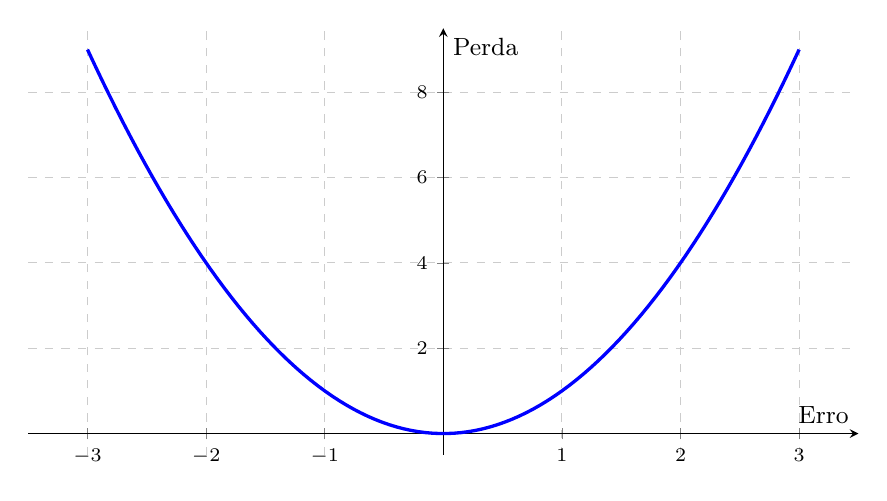
\begin{tikzpicture}
            \begin{axis}[
                % Dimensões ajustadas para caber lado a lado
                width=\linewidth,  
                height=7cm,
                xlabel={Erro},
                ylabel={Perda},
                axis lines=middle,
                grid=major,
                grid style={dashed, gray!40},
                xmin=-3.5, xmax=3.5,
                ymin=-0.5, ymax=9.5,
                legend pos=north west,
                title style={font=\bfseries\small},
                label style={font=\small},
                tick label style={font=\scriptsize}
            ]
                % Gráfico da função x^2
                \addplot[
                    domain=-3:3, 
                    samples=100, 
                    color=blue, 
                    very thick
                ] {x^2};

            \end{axis}
        \end{tikzpicture}
        \caption{Representação gráfica em duas dimensões da função criada.}%
        \label{fig:mse-2d}
    \end{subfigure}
    \hfill 
    \begin{subfigure}[b]{0.48\textwidth}
        \centering
        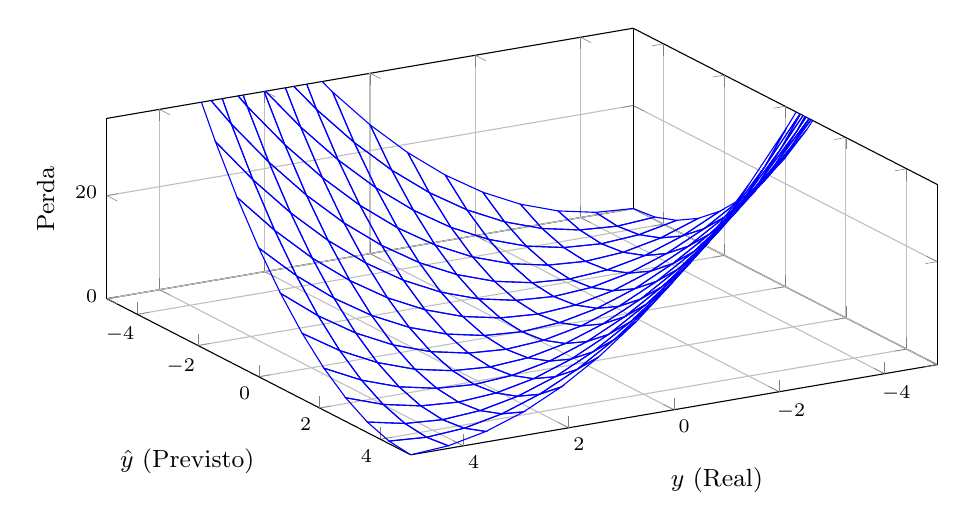
\begin{tikzpicture}
            \begin{axis}[
                % Dimensões consistentes com o gráfico (a)
                width=\linewidth,
                height=7cm,
                xlabel={$y$ (Real)},
                ylabel={$\hat{y}$ (Previsto)},
                zlabel={Perda},
                grid=major,
                view={150}{45}, % Ângulo de visão (azimute, elevação)
                zmin=0, zmax=35, % Ajuste o zmax conforme o domínio
                title style={font=\bfseries\small},
                label style={font=\small},
                tick label style={font=\scriptsize}
            ]
                % Gráfico da superfície (y - y_hat)^2, que é (x - y)^2 no pgfplots
                \addplot3[
                    mesh,           % Tipo de gráfico: superfície
                    color=blue,
                    shader=interp,  % Suaviza as cores
                    domain=-5:5,    % Domínio de x (y_real)
                    domain y=-5:5,  % Domínio de y (y_previsto)
                    samples=15      % Resolução da malha
                ] { (x - y)^2 }; % A função de perda MSE
            \end{axis}
        \end{tikzpicture}
        \caption{Representação gráfica em três dimensões da superfície criada.}%
        \label{fig:mse-3d}
    \end{subfigure}

    \caption{Visualizações da função de perda erro quadrático médio (\textit{MSE}) em duas e em três dimensões.}%
    \label{fig:mse}
    \fonte{O autor (2025).}
\end{figure}

\medskip
\begin{center}
 * * *
\end{center}
\medskip

\textbf{Características do Erro Quadrático Médio}
\vspace{1em}

Tendo os gráficos do erro quadrático médio além de sua equação, cabe agora discutir algumas das principais característica dessa função de perda.

\begin{itemize}
    \item \textbf{Não-negatividade:} Como é visto nos gráficos da Figura~\ref{fig:mse}, o \textit{MSE} é uma função que retorna apenas valores positivos, isso se dá devido a diferença das entradas estar sendo calculada e logo em seguida elevada ao quadrado, impendido que valores negativos ocorram na saída;
    \item \textbf{Sensibilidade para \textit{outliers}:} Como \textcite{LossesArticle} discutem, a função erro quadrático médio possui a tendência de punir em maior força os erros que são originários de uma distância muito grande. Isso acontece por conta do jeito que é calculada essa função, lembre que ela calcula a distância entre os pontos e depois eleva ela ao quadrado, se essa distância for muito grande, o erro será maior ainda. Como consequência, se existe um conjunto grande de pontos que ficam fora da regressão, os \textit{outliers}, a função de perda irá constantemente retornar valores altos. Isso pode atrapalhar o aprendizado, porque será mais difícil otimizar o modelo, mas também pode ser uma vantagem em cenários em que os erros devem ser fortemente penalizados;
    \item \textbf{Convexa (nas predições):} Voltando para a Figura~\ref{fig:mse} é possível notar que o \textit{MSE} é uma função convexa, o seu gráfico tem a típica forma de um funil, apresentando um único ponto de mínimo global, isso ajuda na otimização dessa função caso se esteja usando um otimizador baseado no gradiente descendente. Contudo, \textcite{LossesArticle} destacam que em redes neurais profundas essa função pode se tornar não-convexa, devido as transformações não-lineares que são feitas ao construir o modelo;
    \item \textbf{Baixa interpretabilidade:} Note que a função \textit{MSE} eleva o erro ao quadrado, de forma que ao mostrar a perda não é visto diretamente a distância entre os pontos reais e os pontos preditos pelo modelo. Isso um gera um gargalo pois não é possível de forma instantânea saber exatamente quão bem ou mal o modelo está performando. Funções como a \textit{MAE}, em que o erro é calculado como o módulo da distância entre os dois pontos são mais diretas em mostrar a performance do modelo;
    \item \textbf{Continuidade:} Ainda nos gráficos da Figura~\ref{fig:mse} é possível notar que o \textit{MSE} é uma função contínua em todo o seu domínio, isso é uma vantagem muito boa, pois indica que é possível derivar essa função sem encontrar grandes problemas.
\end{itemize}

\medskip
\begin{center}
 * * *
\end{center}
\medskip

Além disso, cabe também destacar a derivada da função \textit{MSE}, a qual está presente na Equação~\ref{eq:mse-derivada}. A derivada de uma função de perda é de extrema utilizada para uma rede neural, pois é a partir dela que é calculado o primeiro vetor gradiente, e passa a ser retropropagado por toda a rede no sentido inverso, indo primeiro das últimas camadas para as camadas de entrada.

\begin{equacaodestaque}{Derivada Parcial do Erro Quadrático Médio (\textit{MSE}) em Relação a $\hat{y}_j$}
    \frac{\partial\Loss_{\text{MSE}}}{\partial\hat{y}_j} (y_j, \hat{y}_j) = \frac{2}{N} (\hat{y}_j -y_j)%
    \label{eq:mse-derivada}
\end{equacaodestaque}

Note que diferente das funções de ativação em que era calculada a sua derivada ordinária, aqui é calculado as derivadas parciais das funções de perda para cada um dos seus componentes, a saída do modelo $\hat{y}_j$ e a saída esperada $y_j$. Com base nessas duas derivadas, é possível construir o vetor gradiente, como mostrado na Equação~\ref{eq:vetor-gradiente-mse}\footnote{Perceba então que para ter o vetor gradiente completo, deve-se calcular a derivada parcial do \textit{MSE} também em relação os valor real do rótulo ($y_j$). Neste livro será dado um foco maior em apresentar apenas uma das derivas, pois elas muitas vezes apresentarão grandes semelhanças.}.

\begin{equation}
    \nabla (y_j, \hat{y}_j) = \left( \frac{\partial \Loss_{\text{MSE}}}{\partial y_j}, \frac{\partial \Loss_{\text{MSE}}}{\partial \hat{y}_j} \right)%
    \label{eq:vetor-gradiente-mse}
\end{equation}

Considerando a derivada parcial da Equação~\ref{mse-derivada}, é possível construir gráficos como os da Figura~\ref{eq:mse-derivada} para a derivada parcial do \textit{MSE} em relação a $(\hat{y}_j)$. Note também que semelhante as representações do erro quadrático médio, a sua derivada também é apresentada em vistas em duas e três dimensões, isso será algo recorrente nas representações das funções desse capítulo.

\begin{figure}[h!]
    \centering 
    \begin{subfigure}[b]{0.48\textwidth}
        \centering
        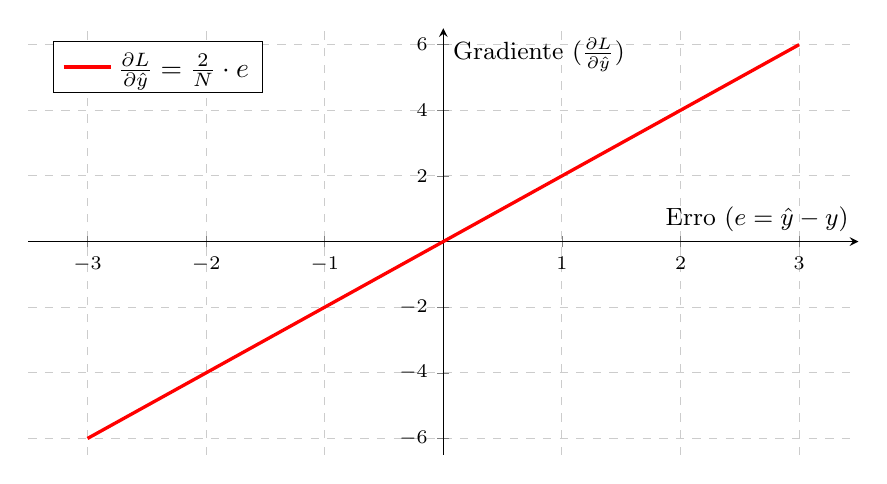
\begin{tikzpicture}
            \begin{axis}[
                width=\linewidth,  
                height=7cm,
                xlabel={Erro ($e = \hat{y} - y$)},
                ylabel={Gradiente ($\frac{\partial L}{\partial \hat{y}}$)},
                axis lines=middle,
                grid=major,
                grid style={dashed, gray!40},
                xmin=-3.5, xmax=3.5,
                ymin=-6.5, ymax=6.5,
                legend pos=north west,
                title style={font=\bfseries\small},
                label style={font=\small},
                tick label style={font=\scriptsize}
            ]
                \addplot[
                    domain=-3:3, 
                    samples=100, 
                    color=red, 
                    very thick
                ] {2*x};
                \addlegendentry{$\frac{\partial L}{\partial \hat{y}} = \frac{2}{N} \cdot e$}
            \end{axis}
        \end{tikzpicture}
        \caption{Visão 2D (Gradiente vs. Erro).}%
        \label{fig:mse-derivada-2d}
    \end{subfigure}
    \hfill 
    \begin{subfigure}[b]{0.48\textwidth}
        \centering
        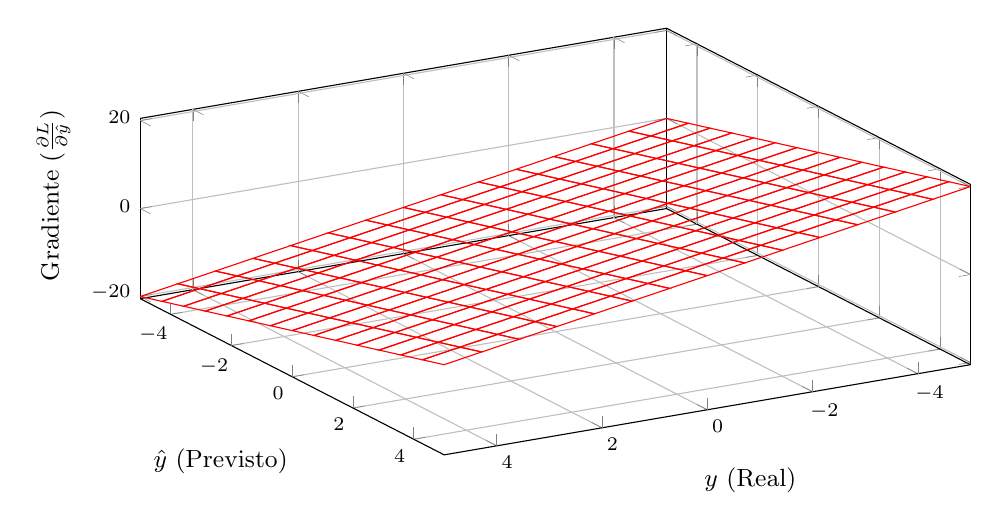
\begin{tikzpicture}
            \begin{axis}[
                width=\linewidth,
                height=7cm,
                xlabel={$y$ (Real)},
                ylabel={$\hat{y}$ (Previsto)},
                zlabel={Gradiente ($\frac{\partial L}{\partial \hat{y}}$)},
                grid=major,
                view={150}{45}, % Mesmo ângulo de visão do seu template
                zmin=-20.5, zmax=20.5, % Ajustado para 2 * (erro máx 10)
                title style={font=\bfseries\small},
                label style={font=\small},
                tick label style={font=\scriptsize}
            ]
                % Gráfico da superfície do gradiente: 2 * (y_hat - y)
                \addplot3[
                    mesh,           
                    color=red,      % Cor consistente com o gráfico 2D
                    shader=interp,  
                    domain=-5:5,    % Mesmo domínio do seu template
                    domain y=-5:5,  % Mesmo domínio do seu template
                    samples=15      % Mesma resolução da malha
                ] { 2 * (y - x) }; % A função da derivada: 2 * (y_previsto - y_real)
            \end{axis}
        \end{tikzpicture}
        \caption{Superfície 3D completa.}%
        \label{fig:mse-derivada-3d}
    \end{subfigure}

    % --- Legenda e Fonte da Figura Principal ---
    \caption{Visualizações da derivada (gradiente) da função de perda MSE.}%
    \label{fig:mse-derivada}
    \fonte{O autor (2025).}
\end{figure}

É possível perceber pelo gráfico da derivada da função de perda erro quadrático médio que o gradiente da perda é proporcional ao erro. Seguindo essa lógica, se o erro está alto, o gradiente também estará alto, como consequência as atualizações de pesos e vieses, as quais seguem o método do gradiente (visto nas Equações~\ref{eq:gradiente-do-erro-em-relacao-a-um-peso-de-um-neuronio-regressao}) serão mais bruscas, dando maiores saltos no gráfico da função de perda. Enquanto em situações que o erro está pequeno em magnitude, o gradiente também será pequeno e o modelo fará pequenas atualizações nos seus parâmetros, garantindo um ajuste fino.

\begin{equation}
    \frac{\partial E}{\partial w_{ji}} = \frac{\partial E}{\partial x_j} \cdot y_i \quad \text{ou} \quad \frac{\partial E}{\partial w_{ji}} = \frac{\partial E}{\partial y_j} \cdot \sigma'(x_j) \cdot y_i
    \label{eq:gradiente-do-erro-em-relacao-a-um-peso-de-um-neuronio-perda-regressao}
\end{equation}

\medskip
\begin{center}
 * * *
\end{center}
\medskip

Antes de discutir algumas aplicações do erro quadrático médio, é interessante introduzir uma função derivada dessa equação: ela é a raiz do erro quadrático médio (\textit{RMSE}). O \textit{RMSE}, como pode ser visto na Equação~\ref{eq:rmse-metric}, é basicamente a introdução de uma raiz quadrada no próprio cálculo do \textit{MSE}. 

\begin{equacaodestaque}{Raíz do Erro Quadrático Médio (\textit{RMSE})}
    {RMSE} (y_j, \hat{y}_j) = \sqrt{\frac{1}{N} \sum_{j=1}^{N} (y_j -\hat{y}_j)^2}%
    \label{eq:rmse-metric}
\end{equacaodestaque}

Essa função tem como objetivo servir de métrica para avaliar os modelos de regressão. O \textit{MSE} funciona como uma função de perda e também como uma métrica avaliativa. Mas como foi dito anteriormente, é difícil interpretar a primeira vista os seus resultados, uma vez que ele eleva ao quadrado o cálculo do erro. Com \textit{RMSE} é resolvido esse ``problema'' da interpretabilidade, dando um resultado mais tangível para entender como o modelo está se comportando. 

Além disso, pode-se pensar que o \textit{RMSE} funcionaria como uma função de perda, mas utilizá-lo nessa estratégia pode não fazer muito sentido, dado que ele tira a principal propriedade do erro quadrático médio: a sensibilidade para \textit{outliers}. 

Dito isso, finalmente é possível discutir algumas aplicações dessas funções em algoritmos de aprendizado de máquina.

\medskip
\begin{center}
 * * *
\end{center}
\medskip

\textbf{Algumas Aplicações do Erro Quadrático Médio em Problemas de Regressão}%
\index{Aplicações práticas! Erro quadrático médio (MSE)}
\vspace{1em}

Além de estar presente nas deduções do algoritmo da retropropagação como uma função de perda, o erro quadrático médio acaba sendo uma função bem versátil para ser aplicada em problemas de regressão. Não somente isso, mas seu uso não se restringe a somente uma função de perda que será utilizada como ``mapa'' para a otimização do modelo, o \textit{MSE} também é uma ótima métrica para avaliar o desempenho de um modelo de regressão. E junto do \textit{MSE} está o \textit{RMSE}, cujo o cálculo é dado pela raiz quadrada do erro quadrático médio. Juntas, essas duas funções se tornam ótimas escolhas para medir como um modelo está performando.

Dito, isso, vale apenas destacar alguns desses cenários em que o erro quadrático médio é utilizado tanto como função de perda, quanto como métrica avaliativa. Além disso, é possível notar que muitas vezes ele irá aparecer indiretamente em formato de raiz do erro quadrático médio.

Assim, algumas aplicações do \textit{MSE} são:

\begin{itemize}
    \item \textbf{Estimação de custos médicos (Saúde):} Em \textit{Medical Costs Estimation Using Linear Regression Method}, \textcite{MedicalCostsEstimationUsingLR} utilizam técnicas de regressão linear como a regressão linear múltipla para fazer previsões de custos médicos. Para avaliar os modelos de regressão criados, os autores fazem uso do erro quadrático médio mas também aplicam outras métricas, como o erro absoluto médio (tópico principal da Seção xx), e também a métrica $R^2$ \parencite{MedicalCostsEstimationUsingLR};
    \item \textbf{Estimação de Preços de Imóveis (Mercado Imobiliário):} No artigo \textit{An Optimal House Price Prediction Algorithm: XGBoost}, \textcite{OptimalHousePricePrediction} aplicam diferentes modelos de regressão (como regressão linear, florestas aleatórias e XGBoost) com intuito de criar um modelo ideal para a prever valores de casas. Com esses diferentes modelos criados, os autores precisaram de diversas métricas para encontrar o modelo ideal, para isso, uma das técnicas foi o uso do \textit{MSE}, além disso, eles utilizam também o \textit{RMSE}, que é dado pelo cálculo da raiz quadrada do próprio erro quadrático médio \parencite{OptimalHousePricePrediction};
    \item \textbf{Previsão da Produção Agrícola (Agronomia):} No trabalho \textit{Coupling Machine Learning and Crop Modeling Improves Crop Yield Prediction in the US Corn Belt}, \textcite{CouplingMachineLearningAndCropModeling} estavam estudando formas de combinar técnicas com modelagem de culturas para prever a produção das plantações na região do cinturão do milho nos Estados Unidos. No artigo, os pesquisadores não utilizam diretamente o \textit{MSE}, ao invés disso, utilizam a raiz do erro quadrático médio como uma das diferentes métricas para avaliação dos modelos de previsão desenvolvidos ao longo do projeto \parencite{CouplingMachineLearningAndCropModeling};
    \item \textbf{Previsão de Demanda de Energia (Gestão Energética):} Já no texto \textit{Optimizing Federated Learning for Scalable Power-demand Forecasting in Microgrids} ocorre uma situação diferente ao aplicar o erro quadrático médio, \textcite{OptimizingFL} fazem uma adaptação nessa função transformando-a no \textit{Exponentially Weighted Mean Squared Error} (\textit{EW-RSM}). Essa adaptação é justificada pelos autores como uma forma de enfatizar a acurácia em previsões de longo prazo atribuindo pesos exponencialmente crescentes aos erros em etapas de tempo posteriores \parencite{OptimizingFL}.
\end{itemize}

\medskip
\begin{center}
 * * *
\end{center}
\medskip

Conhecendo a função de perda \textit{MSE}, é possível agora discutir uma outra abordagem para resolver problemas de regressão. Para isso, a próxima seção busca apresentar o erro absoluto médio, que é uma alternativa para o erro quadrático médio que tem como principal diferença o jeito que lida com \textit{outliers}.

\subsection{Erro Absoluto Médio (MAE)}%
\index{Funções de Perda!Erro Absoluto Médio (MAE)}%
\label{sec:mae-loss}

O \gls{mae-loss}, também chamado de perda L1, é uma função que tem o mesmo propósito do erro quadrático médio, ser utilizada para tarefas de regressão. Neste caso o \textit{MAE} não possui uma origem definida que como o \textit{MSE}, esse conceito de minimizar a diferença de um resultado pelo seu valor real já havia sendo utilizado a bastante tempo. Contudo, trabalhos como \textit{Greedy function approximation: A gradient boosting machine} de \textcite{GreedyFunctionApproximation} fazem uso do erro absoluto médio para resolver problemas de aprendizado de máquina. No texto, o autor desenvolve um algoritmo de \textit{boosting} específico para o \textit{MAE}, neste caso, essa função é apresentada com outro nome, \textit{Least-Absolute-Deviation} (\textit{LAD}), sendo responsável por dar nome ao algoritmo criado, o \texttt{LAD\_TreeBoost} \parencite{GreedyFunctionApproximation}. Neste caso, \textcite{GreedyFunctionApproximation} explica que esse algoritmo faz uso de uma árvore de regressão com a perda, de forma que para prever a pseudo-resposta que é o sinal dos resíduos atuais é utilizado o método dos mínimos quadrados. Assim, o modelo é atualizado adicionando em cada nó terminal da nova árvore criada a mediana dos resíduos daquela região específica.

Um trabalho mais recente que explora o uso dessa função é o \textit{Image-to-Image Translation with Conditional Adversarial Networks} \parencite{ImageToImage}. Nele, \textcite{ImageToImage} argumentam que preferiram trabalhar com a função de perda \textit{L1 distance} (um dos diferentes nomes utilizados para se referir ao \textit{MAE}) devido a essa função gerar imagens menos borradas. É possível ver essa comparação nas imagens da Figura~\ref{fig:comparativo-perdas-image-to-image}. Perceba que a perda que apresenta os resultados mais consistentes com a realidade é justamente a \textit{L1 + cGAN}, a qual possuí o \textit{MAE} em sua composição.

\begin{figure}[h]
    \centering
    \includegraphics[width=0.65\linewidth]{../imagens/perda-regressao/image-to-image-perdas-comparativo.png}
    
    \caption[Perdas diferentes induzem qualidades de resultados diferentes. Cada coluna mostra resultados treinados sob uma perda diferente de aprendizado no dataset MNIST]{%
        \newline
        \small Fonte: \parencite{ImageToImage}.
    }%
    \label{fig:comparativo-perdas-image-to-image}
\end{figure}

Além disso, vale a pena destacar como o erro absoluto médio se enquadra no exemplo ilustrativo do jogo dos dardos. Para isso, diferente do erro quadrático médio, em que quanto mais longe do centro, o número de pontos perdidos aumentava de forma quadrática, no \textit{MAE} a penalização com relação aos jogadores ruins é mais suave, sendo dada de forma linear. 

Além disso, é interessante fazer uma outra analogia considerando o cenário em que o \textit{MAE} se encontra. Para isso, é preciso considerar que será feito um novo jogo de dardos com dez participantes, em que cada um tem direito de jogar apenas um dardo, e que no final os dez dardos serão somados e com base neles será dado o resultado da equipe. Se tivéssemos uma equipe muito ruim utilizando como métrica o \textit{MSE} para avaliar os pontos, o resultado seria péssimo, porque esses dardos estariam muito longes do centro, e como o erro é elevado ao quadrado, isso geraria uma pontuação muito baixa. 

Contudo, se a métrica escolhida para avaliar o jogo fosse o \textit{MAE} o resultado seria bem melhor, visto que o erro cresce de forma linear. Saindo da alogia e voltando para o cenário de aprendizado de máquina, é possível associar os jogadores ruins com os \textit{outliers}, eles estão presentes nos dados e vão atrapalhar o aprendizado do seu modelo. Contudo, escolher uma função que não seja tão agressiva na medição desses \textit{outliers} pode ser uma excelente alternativa para trabalhar em cenários em que essa configuração será muito comum.

Visto esses diferentes cenários em que o erro absoluto médio foi utilizado para resolver problemas de regressão, além de como ele pode ser associado com o jogo dos dardos, é possível ver agora a sua definição matemática. Para isso, o \textit{MAE} está definido na Equação~\ref{eq:mae}. Perceba que ele é responsável por calcular a diferença entre os dois pontos, o valor real $\hat{y}_j$ e o valor predito $y_j$, para todos os $N$ casos analisados e a partir disso calcular a média dos resultados.

\begin{equacaodestaque}{Erro Absoluto Médio (\textit{MAE})}
    \Loss_{\text{MAE}} (y_j, \hat{y}_j) = \frac{1}{N} \sum_{j=1}^{N} |y_j -\hat{y}_j|%
    \label{eq:mae}
\end{equacaodestaque}

Em que:

\begin{itemize}
    \item $y_j$ representa o valor real da j-ésima amostra;
    \item $\hat{y}_j$ representa o valor predito pelo modelo;
    \item $N$ representa o número de amostras.
\end{itemize}


Também vale a pena analisar o erro absoluto médio de forma gráfica. Para isso, suas representações em duas e três dimensões estão presentes na Figura~\ref{fig:mae} de forma semelhante ao que foi feito ao apresentar o \textit{MSE}.

\begin{figure}[h!]
    \centering
    \begin{subfigure}[b]{0.48\textwidth}
        \centering
        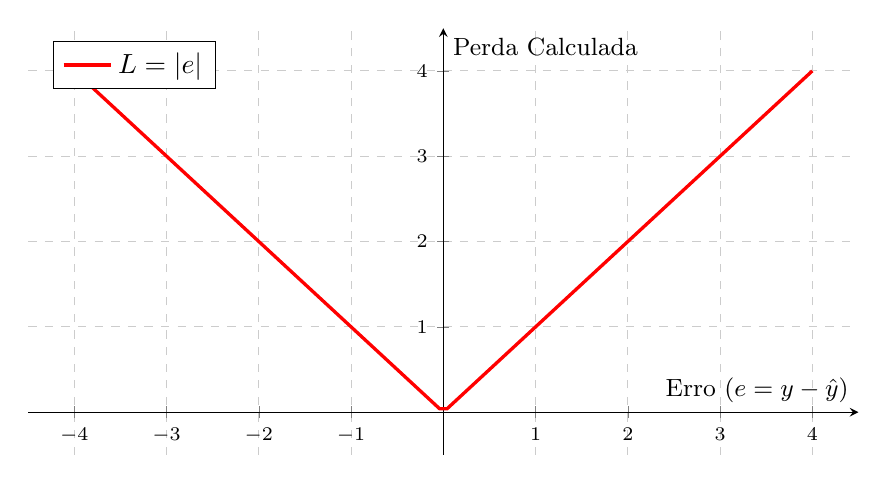
\begin{tikzpicture}
            \begin{axis}[
                % Dimensões ajustadas para caber lado a lado
                width=\linewidth,  
                height=7cm,
                xlabel={Erro ($e = y - \hat{y}$)},
                ylabel={Perda Calculada},
                axis lines=middle,
                grid=major,
                grid style={dashed, gray!40},
                xmin=-4.5, xmax=4.5,        % Limites do seu gráfico MAE
                ymin=-0.5, ymax=4.5,         % Limites do seu gráfico MAE
                legend pos=north west,
                title style={font=\bfseries\small},
                label style={font=\small},
                tick label style={font=\scriptsize}
            ]
                % Gráfico da função abs(x)
                \addplot[
                    domain=-4:4, 
                    samples=100, 
                    color=red, 
                    very thick
                ] {abs(x)};
                
                \addlegendentry{$L = |e|$}
            \end{axis}
        \end{tikzpicture}
        \caption{Representação gráfica em duas dimensões.}%
        \label{fig:mae-2d}
    \end{subfigure}
    \hfill
    \begin{subfigure}[b]{0.48\textwidth}
        \centering
        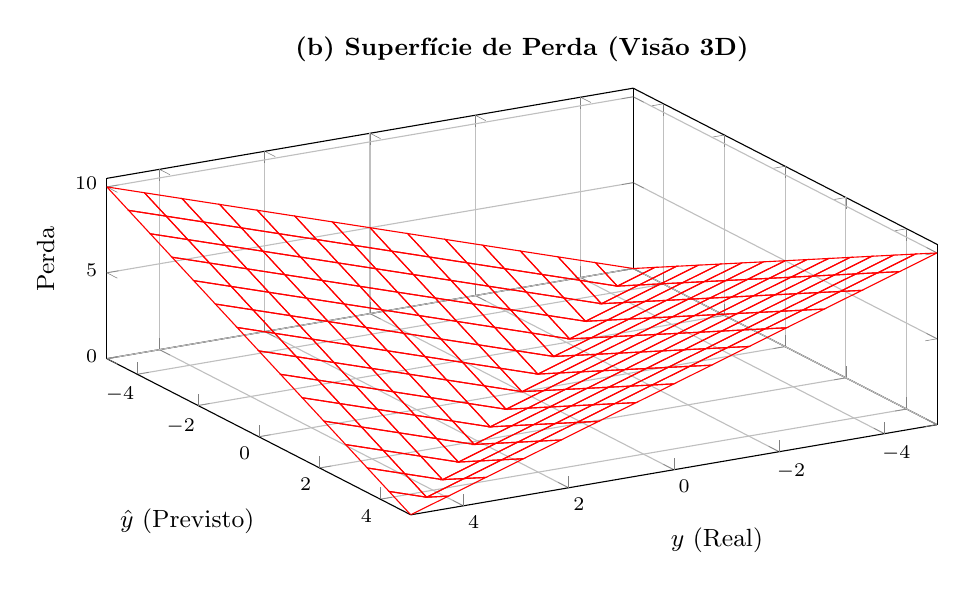
\begin{tikzpicture}
            \begin{axis}[
                % Dimensões consistentes com o gráfico (a)
                width=\linewidth,
                height=7cm,
                title={(b) Superfície de Perda (Visão 3D)},
                xlabel={$y$ (Real)},
                ylabel={$\hat{y}$ (Previsto)},
                zlabel={Perda},
                grid=major,
                view={150}{45}, % Mesmo ângulo de visão do seu template
                zmin=0, zmax=10.5, % Limite Z ajustado para o MAE (abs(-5 - 5) = 10)
                title style={font=\bfseries\small},
                label style={font=\small},
                tick label style={font=\scriptsize}
            ]
                % Gráfico da superfície abs(y - y_hat)
                \addplot3[
                    mesh,           
                    color=red,      % Cor consistente com o gráfico 2D
                    shader=interp,  
                    domain=-5:5,    % Mesmo domínio do seu template
                    domain y=-5:5,  % Mesmo domínio do seu template
                    samples=15      % Mesma resolução da malha
                ] { abs(x - y) }; % A função de perda MAE
            \end{axis}
        \end{tikzpicture}
        \caption{Representação gráfica em três dimensões.}%
        \label{fig:mae-3d}
    \end{subfigure}

    % --- Legenda e Fonte da Figura Principal ---
    \caption{Visualizações da função de perda erro absoluto médio (\textit{MAE}) em duas e em três dimensões.}%
    \label{fig:mae}
    \fonte{O autor (2025).}
\end{figure}

\medskip
\begin{center}
 * * *
\end{center}
\medskip

\textbf{Características do Erro Absoluto Médio}
\vspace{1em}

A partir do seu gráfico e de sua equação é possível retirar diferentes informações dessa função de perda, as quais estão discutidas a seguir:

\begin{itemize}
    \item \textbf{Não-negatividade:} Como é possível ver em seu gráfico da Figura~\ref{fig:mae}, o erro absoluto médio compartilha dessa mesma propriedade com o \textit{MSE}, isso significa que sua saída será sempre positiva ou zero, independente do valor de entrada. Isso se dá, devido a propriedade do módulo, que não admite números negativos para sua saída;
    \item \textbf{Robustez para \textit{outliers}}: Como \textcite{LossesArticle} explicam, o \textit{MAE} não penaliza os \textit{outliers} de forma tão severa como o erro quadrático médio. Isso acontece pois diferente do \textit{MSE}, em que o erro cresce de forma quadrática, no \textit{MAE}, ele cresce de forma linear, significando que diferente do \textit{MSE} que era sensível aos \textit{outliers}, o \textit{MAE} também reage à eles, mas de forma menos severa;
    \item \textbf{Convexa (nas predições):} Voltando para o seu gráfico, é possível ver que o erro absoluto médio segue a mesma forma de funil do erro quadrático médio, podendo ser considerado uma função convexa e com um só ponto de mínimo global. Contudo, assim como no \textit{MSE}, \textcite{LossesArticle} advertem que para modelos de aprendizado profundo, o \textit{MAE} pode deixar de ser uma função convexa devido às muitas camadas e funções não-lineares;
    \item \textbf{Não-derivável em zero:} Esse ponto acontece justamente devido a forma que a função apresenta, ela faz uma espécie de ``bico'' em zero, além disso, ao calcular os seus limites laterais para verificar a continuidade da função é possível notar que eles apresentam valores diferentes;
    \item \textbf{Boa interpretabilidade:} Diferente do erro quadrático médio em que o erro total é elevado ao quadrado, no \textit{MAE} isso não ocorre, o erro é simplesmente a média das diferenças dos pontos. Isso significa que é mais fácil interpretar os resultados que essa função de perda retorna, pois não é preciso fazer nenhum cálculo adicional para ter uma ideia precisa se as previsões feitas pelo modelo estão longe ou não dos valores reais;
\end{itemize}

\medskip
\begin{center}
 * * *
\end{center}
\medskip

Como foi destacado anteriormente, o \textit{MAE} não é derivável em zero. Inicialmente pode ter-se a ideia de que devido a isso, essa não seja uma função boa para ser utilizada em conjunto com otimizadores baseados em gradiente, porque pontos de descontinuidade como este podem acabar atrapalhando a forma como o modelo é otimizado. Contudo, \textcite{LossesArticle} argumentam, é possível resolver esse problema utilizado técnicas de subgradiente, sendo possível então escrever a derivada do \textit{MAE} com a Equação~\ref{eq:mae-derivada}.

\begin{equacaodestaque}{Derivada Parcial do Erro Absoluto Médio (\textit{MAE}) em Relação a $\hat{y}_j$}
    \frac{\partial\Loss_{\text{MAE}}}{\partial\hat{y}_j} (y_j, \hat{y}_j) = 
    \begin{cases} 
      -1 & \text{se } \hat{y}_j > y_j \\
      +1 & \text{se } \hat{y}_j < y_j \\
      [-1, +1] & \text{se } \hat{y}_j = y_j
    \end{cases}%
    \label{eq:mae-derivada}
\end{equacaodestaque}

Contudo, mesmo possuindo esse detalhe de descontinuidade em zero, isso não atrapalha a plotagem do gráfico do \textit{MAE}, o qual está representado na Figura~\ref{fig:mae-derivada}. De forma semelhante ao que foi feito até agora, na figura da esquerda, a Figura~\ref{fig:mae-derivada-2d}, está a representação em duas dimensões dessa função, enquanto na figura da direta, a Figura~\ref{fig:mae-derivada-3d}.

\begin{figure}[h!]
    \centering
    \begin{subfigure}[b]{0.48\textwidth}
        \centering
        \begin{tikzpicture}
            \begin{axis}[
                % Dimensões ajustadas para caber lado a lado
                width=\linewidth,  
                height=7cm,
                xlabel={Erro ($e = \hat{y} - y$)},
                ylabel={Gradiente ($\frac{\partial L}{\partial \hat{y}}$)},
                axis lines=middle,
                grid=major,
                grid style={dashed, gray!40},
                xmin=-3.5, xmax=3.5,        % Limites do seu gráfico
                ymin=-1.5, ymax=1.5,         % Limites do seu gráfico
                ytick={-1, 0, 1},           % Pontos no eixo y
                legend pos=north west,
                title style={font=\bfseries\small},
                label style={font=\small},
                tick label style={font=\scriptsize}
            ]
                % Parte negativa da derivada (-1)
                \addplot[
                    domain=-3:0, 
                    samples=100, 
                    color=red, 
                    very thick
                ] {-1};

                % Parte positiva da derivada (+1)
                \addplot[
                    domain=0:3, 
                    samples=100, 
                    color=red, 
                    very thick
                ] {1};
                
                % Círculos abertos para a descontinuidade em x=0
                \addplot[only marks, mark=o, color=red, mark size=2pt] coordinates {(0,-1) (0,1)};
            \end{axis}
        \end{tikzpicture}
        \caption{Visão 2D (Gradiente vs. Erro).}%
        \label{fig:mae-derivada-2d}
    \end{subfigure}
    \hfill 
    \begin{subfigure}[b]{0.48\textwidth}
        \centering
        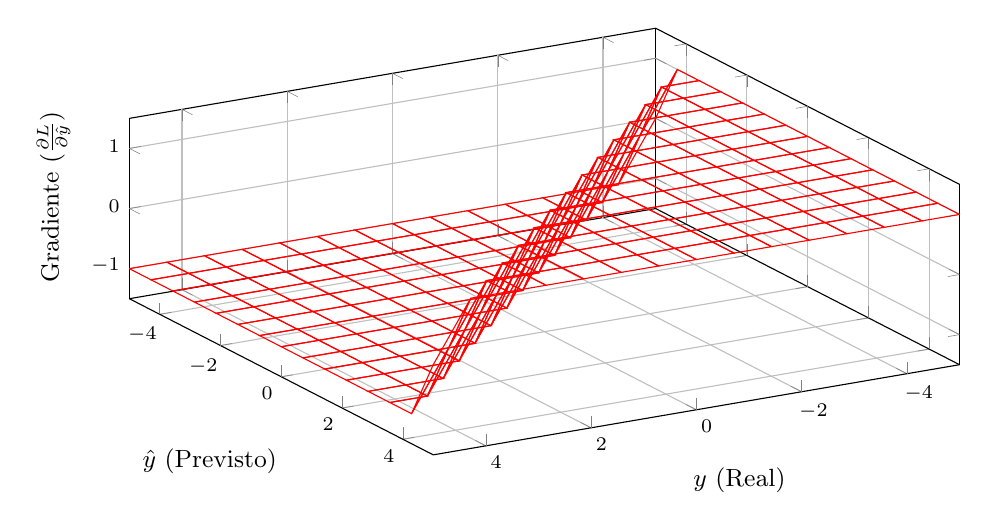
\begin{tikzpicture}
            \begin{axis}[
                % Dimensões consistentes com o gráfico (a)
                width=\linewidth,
                height=7cm,
                xlabel={$y$ (Real)},
                ylabel={$\hat{y}$ (Previsto)},
                zlabel={Gradiente ($\frac{\partial L}{\partial \hat{y}}$)},
                grid=major,
                view={150}{45}, % Mesmo ângulo de visão do seu template
                zmin=-1.5, zmax=1.5, % Espelha o eixo Y do gráfico 2D
                ztick={-1, 0, 1}, % Consistente com o 2D
                title style={font=\bfseries\small},
                label style={font=\small},
                tick label style={font=\scriptsize}
            ]
                % Gráfico da superfície do gradiente: sign(y_hat - y)
                \addplot3[
                    mesh,           
                    color=red,      % Cor consistente com o gráfico 2D
                    shader=interp,  
                    domain=-5:5,    % Mesmo domínio do seu template
                    domain y=-5:5,  % Mesmo domínio do seu template
                    samples=15      % Mesma resolução da malha
                ] { sign(y - x) }; % A função da derivada: sign(y_previsto - y_real)
            \end{axis}
        \end{tikzpicture}
        \caption{Superfície 3D completa.}%
        \label{fig:mae-derivada-3d}
    \end{subfigure}

    % --- Legenda e Fonte da Figura Principal ---
    \caption{Visualizações da derivada (gradiente) da função de perda MAE.}%
    \label{fig:mae-derivada} % Rótulo principal do seu gráfico
    \fonte{O autor (2025).}
\end{figure}

Perceba que a derivada do erro absoluto médio é representado em forma de uma função por partes, neste caso, ela é divida em duas diferentes retas, parecida com a função de ativação degrau unitário. Note também que existe um ``bico'' na união dessas duas retas, isso acontece devido a descontinuidade dessa função em zero, o que impede de ser derivada nesse ponto. Assim, a derivada do \textit{MAE} pode ser interpretada como a composição de duas retas constantes, a primeira constante em -1, e a segunda constante em 1.

\medskip
\begin{center}
 * * *
\end{center}
\medskip

\textbf{Algumas Aplicações do Erro Absoluto Médio em Problemas de Regressão}%
\index{Aplicações práticas! Erro absoluto médio (MAE)}
\vspace{1em}

Além dos casos discutidos no início da seção: o \texttt{LAD\_TreeBoost} e o artigo \textit{Image-to-Image Translation with Conditional Adversarial Networks}, o \textit{MAE} também está presente em uma série de trabalhos, atuando tanto como função de perda, quanto servindo como uma métrica de avaliação, indicando se o modelo desenvolvido está performando bem ou não. Dito isso, essa seção busca explorar algumas dessas aplicações do erro absoluto médio, semelhante ao que foi feito ao analisar o erro quadrático médio. 

Dito isso, vale destacar os trabalhos:

\begin{itemize}
    \item \textbf{Avaliação de idade óssea e estimação do escore de cálcio na artéria coronária (Saúde):} Em \textit{Regression Metric Loss: Learning a Semantic Representation Space for Medical Images}, \textcite{chao2022regressionmetriclosslearning} desenvolvem algoritmos de regressão para estimar escore de cálcio da artéria coronária e também um segundo algoritmo para avaliação da idade óssea. Além disso, os autores apresentam uma nova função de perda, a \textit{RM-Loss} que demonstra ser mais apta para resolver os problemas propostos de regressão \parencite{chao2022regressionmetriclosslearning}. Como forma de avaliar essa nova função criada e também as diferentes outras funções comparadas no artigo, \textcite{chao2022regressionmetriclosslearning} utilizam o erro absoluto médio como uma das métricas;
    \item \textbf{Restauração de imagens (Engenharia):} No artigo \textit{Noise2Noise: Learning Image Restoration without Clean Data}, \textcite{Noise2Noise} estavam estudando formas de restaurar imagens corrompidas sem a utilização de dados limpos. Em um dos experimentos os autores estavam buscando uma forma ideal de remover textos de imagens, de forma que a perda L1, por ser uma função de perda robusta, conseguiu atingir bons resultados nessa tarefa \parencite{Noise2Noise};
    \item \textbf{Previsão da produção de energia eólica (Setor energético):} Já em \textit{Minimum Open Data Subset for Wind Power Prediction}, \textcite{MinimumOpenDataSubsetForWindPowerPrediction} utilizam um modelo de florestas aleatórias com o objetivo de prever a produção de energia eólica. Para avaliar o modelo de regressão desenvolvido, os autores utilizam como métricas o \textit{MAE} além do \textit{RMSE}. Além disso, vale comentar que em testes realizados pelos pesquisadores foi possível criar um modelo com erro absoluto médio de 0,071, indicando um excelente resultado para para o algoritmo criado \parencite{MinimumOpenDataSubsetForWindPowerPrediction}.
    \item \textbf{Previsão de poluição do ar (Setor ambiental):} Por fim, vale a pena destacar o trabalho de \textcite{nedungadi2025aircastimprovingairpollution}, \textit{AirCast: Improving Air Pollution Forecasting Through Multi-Variable Data Alignment}, em que os autores buscam formas de melhorar a previsão da poluição do ar. Como forma de ajudar a resolver esse problema, os autores utilizam uma função inspirada pelo erro absoluto médio, o \textit{Frequency-weighted Mean Absolute Error} (\textit{fMAE}), que tem como principal vantagem lidar com variáveis que apresentam uma distribuição de cauda pesada, como as variáveis PM1, PM2.5 e PM10, que indicam a qualidade do ar \parencite{nedungadi2025aircastimprovingairpollution}.
\end{itemize}

\medskip
\begin{center}
 * * *
\end{center}
\medskip

Visto o erro quadrático médio, que penaliza fortemente ou \textit{outliers}, e o erro absoluto médio, que não penaliza de forma agressiva os \textit{outliers}, surge uma pergunta: Existe alguma forma de ter uma função que penalize os erros gravemente até um certo ponto e depois desse, ela não se preocupe tanto com os \textit{outliers}? Essa é a proposta da perda de Huber, a qual busca unir os principais benefícios dessas duas funções de regressão. Ela é o tópico principal da próxima seção.

\subsection{Perda de Huber (Huber Loss)}%
\index{Funções de Perda!Perda de Huber (Huber Loss)}%
\label{sec:huber-loss}

A \gls{huber-loss} recebe o seu nome devido ao seu criador, Peter J. Huber, que apresentou para a comunidade científica no trabalho \textit{Robust Estimation of a Location Parameter} \parencite{HuberLoss}. No artigo, \textcite{HuberLoss}, estava estudando maneiras de fazer uma estimação robusta de um parâmetro de localização (como a média o mediana de um conjunto de dados) quando a distribuição dos dados é aproximadamente conhecida. Além disso, no trabalho, o autor define um estimador robusto $p$ que segue a Equação~\ref{eq:huber-loss-do-huber}, a qual prova ser uma solução ideal para o problema estudado \parencite{HuberLoss}.

\begin{equation}
    \rho(t) = 
    \begin{cases}
        \frac{1}{2} t^2 & \text{se} |t| < k \\
        k |t| - \frac{1}{2} k^2 & \text{se} t \ge k
    \end{cases}
    \label{eq:huber-loss-do-huber}
\end{equation}

O que Huber estava querendo basicamente com a Equação~\ref{eq:huber-loss-do-huber} era uma função que se comportasse de forma quadrática para os casos em que $|t| < k$ e que se comportasse de forma linear para os casos em que $t \ge k$. Essa função criada pelo pesquisador é a função que está sendo estudada, a perda de Huber, a qual pode ser representada, agora com notações voltadas para o cenário de aprendizado de máquina, com a Equação~\ref{eq:huber-loss}.

\begin{equacaodestaque}{Perda de Huber (Huber \textit{Loss})}
    \Loss_{\text{Huber}} (y, \hat{y}) = 
    \begin{cases} 
      \frac{1}{2} (y -\hat{y})^2 & \text{para } |y -\hat{y}| \le\delta\\
      \delta(|y -\hat{y}| -\frac{1}{2}\delta) & \text{caso contrário}
    \end{cases}%
    \label{eq:huber-loss}
\end{equacaodestaque}

Em que:

\begin{itemize}
    \item $y_j$ representa o valor real da j-ésima amostra;
    \item $\hat{y}_j$ representa o valor predito pelo modelo;
    \item $N$ representa o número de amostras;
    \item $\delta$ representa
\end{itemize}

É possível também representar a perda de Huber utilizando gráficos, para isso, ela pode ser vista na Figura~\ref{fig:huber-loss}. Para isso, na Figura~\ref{fig:huber-2d} está representado a visualização em duas dimensões dessa função, enquanto na Figura~\ref{fig:huber-3d} está a representação no espaço da superfície, assim como o que vem sendo feito até agora. Perceba que é como se ela fosse duas funções em uma, até um certo ponto do gráfico ela age parecido a uma função quadrática, contudo, após passar do limite de $\delta$ ela passa a ser uma função linear.

\begin{figure}[h!]
    \centering
    \begin{subfigure}[b]{0.48\textwidth}
        \centering
        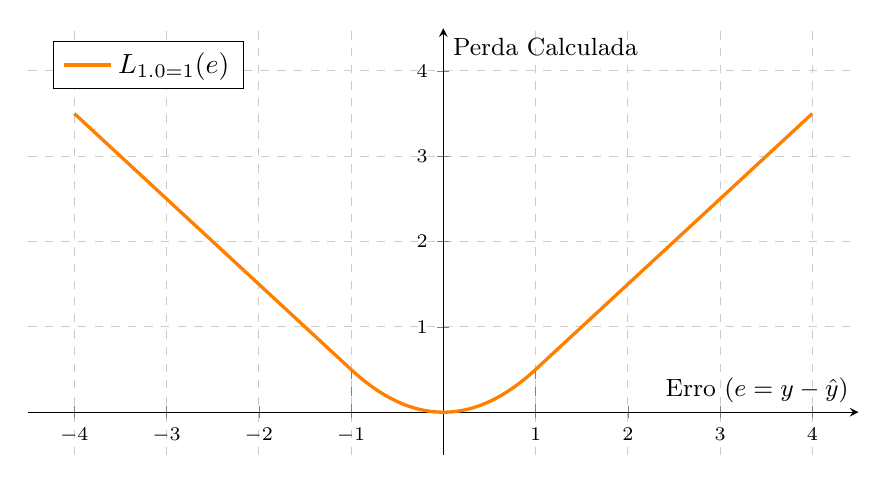
\begin{tikzpicture}
            % Define o valor de delta para este gráfico
            \def\delta{1.0} 
            
            \begin{axis}[
                % Dimensões ajustadas para caber lado a lado
                width=\linewidth,  
                height=7cm,
                xlabel={Erro ($e = y - \hat{y}$)},
                ylabel={Perda Calculada},
                axis lines=middle,
                grid=major,
                grid style={dashed, gray!40},
                xmin=-4.5, xmax=4.5,        % Limites do seu gráfico
                ymin=-0.5, ymax=4.5,         % Limites do seu gráfico
                legend pos=north west,
                title style={font=\bfseries\small},
                label style={font=\small},
                tick label style={font=\scriptsize}
            ]
                % Gráfico da função Huber Loss
                \addplot[
                    domain=-4:4, 
                    samples=201, 
                    color=orange, 
                    very thick
                ] { abs(x) <= \delta ? 0.5*x^2 : \delta*(abs(x) - 0.5*\delta) };
                
                \addlegendentry{$L_{\delta=1}(e)$}

                % Linhas de transição em delta
                \draw[dashed, gray] (axis cs:-\delta, 0) -- (axis cs:-\delta, {\delta*(\delta-0.5*\delta)});
                \draw[dashed, gray] (axis cs:\delta, 0) -- (axis cs:\delta, {\delta*(\delta-0.5*\delta)});
            \end{axis}
        \end{tikzpicture}
        \caption{Representação gráfica em duas dimensões.}%
        \label{fig:huber-2d}
    \end{subfigure}
    \hfill 
    \begin{subfigure}[b]{0.48\textwidth}
        \centering
        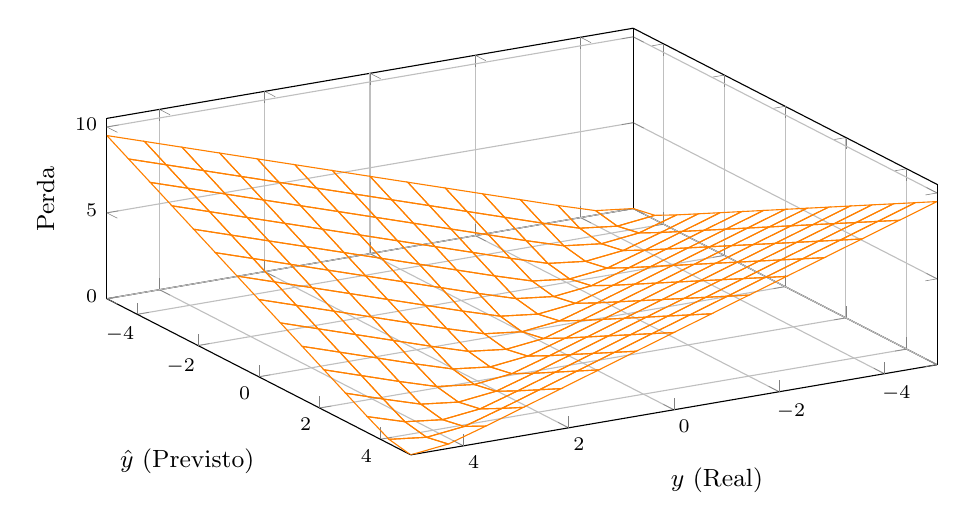
\begin{tikzpicture}

            \def\delta{1.0}
            
            \begin{axis}[
                % Dimensões consistentes com o gráfico (a)
                width=\linewidth,
                height=7cm,
                xlabel={$y$ (Real)},
                ylabel={$\hat{y}$ (Previsto)},
                zlabel={Perda},
                grid=major,
                view={150}{45}, % Mesmo ângulo de visão do seu template
                zmin=0, zmax=10.5, % Limite Z ajustado para Huber com domínio -5:5
                title style={font=\bfseries\small},
                label style={font=\small},
                tick label style={font=\scriptsize}
            ]
                % Gráfico da superfície da Huber Loss
                \addplot3[
                    mesh,           
                    color=orange,   % Cor consistente com o gráfico 2D
                    shader=interp,  
                    domain=-5:5,    % Mesmo domínio do seu template
                    domain y=-5:5,  % Mesmo domínio do seu template
                    samples=15      % Mesma resolução da malha
                ] { abs(x-y) <= \delta ? 0.5*(x-y)^2 : \delta*(abs(x-y) - 0.5*\delta) }; % A função Huber 3D
            \end{axis}
        \end{tikzpicture}
        \caption{Representação gráfica em três dimensões.}%
        \label{fig:huber-3d}
    \end{subfigure}

    \caption{Visualizações da função de perda de Huber (\textit{Huber Loss}, $\delta=1$) em duas e em três dimensões.}%
    \label{fig:huber-loss}
    \fonte{O autor (2025).}
\end{figure}

Um ponto a ser destacado ao utilizar a perda de Huber é com relação a escolha de valores para o parâmetro $\delta$. Um valor muito pequeno para $\delta$ faz com que a função se comporte mais como o erro absoluto médio, é possível ver essa situação na Figura~\ref{fig:huber-comparacoes-mae}, já ao escolher um valor muito grande para $\delta$ faz com que a perda de Huber se assemelhe mais a função erro quadrático médio, essa situação está na Figura~\ref{fig:huber-comparacoes-mse}. \textcite{LossesArticle} explicam que a escolha de valores para $\delta$ pode ser feita de forma empírica, através de validação cruzada (\textit{cross-validation}). Assim, testes são recomendados a fim de escolher o melhor valor para $\delta$ no cenário em que está sendo trabalhado.

\begin{figure}[h!]
    \centering
    \begin{subfigure}[b]{0.48\textwidth}
        \centering
        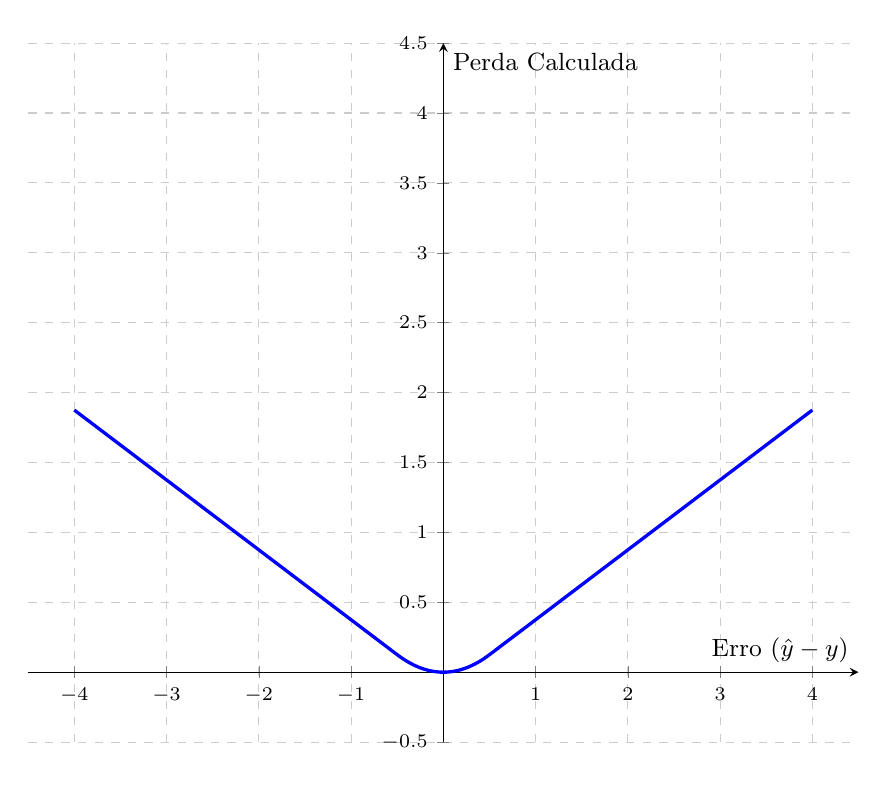
\begin{tikzpicture}
            \def\delta{0.5} % Delta pequeno
            \begin{axis}[
                xlabel={Erro ($\hat{y} - y$)},
                ylabel={Perda Calculada},
                axis lines=middle,
                grid=major,
                grid style={dashed, gray!40},
                xmin=-4.5, xmax=4.5,
                ymin=-0.5, ymax=4.5,
                legend pos=north west,
                width=\textwidth,
                label style={font=\small},
                tick label style={font=\scriptsize},
                title style={font=\bfseries, yshift=-5pt},
            ]
                % Função Huber Loss
                \addplot[
                    domain=-4:4, 
                    samples=201, 
                    color=blue, 
                    very thick,
                ] {(abs(x) <= \delta) ? (0.5*x^2) : (\delta*(abs(x) - 0.5*\delta))};
            \end{axis}
        \end{tikzpicture}
        \caption{Perda Huber com $\delta = 0.5$.}%
        \label{fig:huber-comparacoes-mae}
    \end{subfigure}
    \hfill
    \begin{subfigure}[b]{0.48\textwidth}
        \centering
        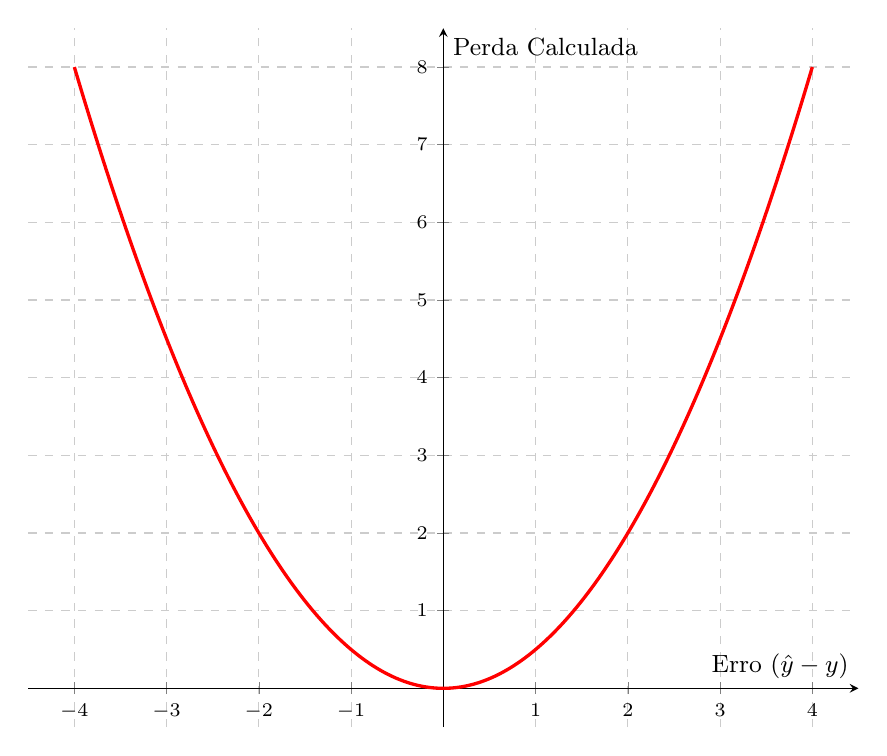
\begin{tikzpicture}
            \def\delta{4.0} % Delta grande
            \begin{axis}[
                xlabel={Erro ($\hat{y} - y$)},
                ylabel={Perda Calculada},
                axis lines=middle,
                grid=major,
                grid style={dashed, gray!40},
                xmin=-4.5, xmax=4.5,
                ymin=-0.5, ymax=8.5,
                legend pos=north west,
                width=\textwidth,
                label style={font=\small},
                tick label style={font=\scriptsize},
                title style={font=\bfseries, yshift=-5pt},
            ]
                % Função Huber Loss
                \addplot[
                    domain=-4:4, 
                    samples=201, 
                    color=red, 
                    very thick
                ] {(abs(x) <= \delta) ? (0.5*x^2) : (\delta*(abs(x) - 0.5*\delta))};

            \end{axis}
        \end{tikzpicture}
        \caption{Perda Huber com $\delta = 4.0$.}%
        \label{fig:huber-comparacoes-mse}
    \end{subfigure}
    
    \caption{Comparação da Perda de Huber com diferentes valores de $\delta$.}%
    \label{fig:huber-delta-comparacoes}
    \fonte{O autor (2025).}
\end{figure}

Assim, nota-se que ao utilizar a perda de Huber em um problema de regressão, é nítido que o grau de complexidade do problema pode aumentar, pois haverá mais um hiperparâmetro para ser otimizado de forma manual. Isso pode não ser ideal para cenários em que já existem muitos hiperparâmetros. Para isso, \textcite{LossesArticle} explicam que essa função é comumente utilizada em problemas de regressão robusta, como em regressões lineares e em previsão de séries temporais (\textit{time series forecasting}), em que \textit{outliers} e ruído podem estar presentes.

\medskip
\begin{center}
 * * *
\end{center}
\medskip

\textbf{Características da Perda de Huber}
\vspace{1em}

Conhecido o gráfico e sua equação, é possível agora discutir algumas das propriedades da perda de Huber, as quais são apresentadas a seguir:

\begin{itemize}
    \item \textbf{Robustez para \textit{outliers}:} Assim como o \textit{MAE}, a perda de Huber não penaliza de forma quadrática os erros como comparado com o erro quadrático médio, dessa forma, os \textit{outliers} não conseguem afetar drasticamente o cálculo da perda dependendo do valor de $\delta$ escolhido \parencite{LossesArticle};
    \item \textbf{Diferenciabilidade em $\delta$:} Um ponto a ser destacado ao se utilizar a perda Huber é que ela apresenta pontos de descontinuidade para o cenário em que $y - \hat{y} = \delta$, contudo a função é contínua em todo o resto, dessa forma, isso não a impede de ser utilizada em conjunto com otimizadores baseados em gradiente \parencite{LossesArticle};
    \item \textbf{Convexa:} Bem como as funções de perda vistas até agora, a perda de Huber também é uma função convexa. Isso pode ser visto nos gráficos da Figura~\ref{fig:huber-loss}, note que ela segue a forma clássica de uma funil, comum em funções convexas. Essa característica é uma vantagem para a perda de Huber, pois facilita com que os otimizadores encontrem os pontos de mínimo. Contudo, em redes neurais isso é mais complicado, devido as transformações não-lineares que ocorrem no modelo, fazendo com que a função de perda deixe de ser convexa.
\end{itemize}

\medskip
\begin{center}
 * * *
\end{center}
\medskip

Cabe também discutir a diferenciabilidade da perda de Huber, e como é dado o cálculo do seu gradiente. Dito isso, como explicam \textcite{LossesArticle}, o gradiente da perda de Huber deve ser calculado por partes, sendo que é possível utilizar a Equação~\ref{eq:huber-loss-derivada} como guia.

\begin{equacaodestaque}{Derivada Parcial da Perda de Huber (Huber \textit{loss}) em Relação a $\hat{y}$}
    \frac{\partial\Loss_{\delta}}{\partial\hat{y}} (y_j, \hat{y}_j) = 
    \begin{cases} 
        \hat{y} -y & \text{se } | y -\hat{y} | \le\delta\\
        \delta\cdot \text{sgn} (\hat{y} -y) & \text{se } | y -\hat{y} | > \delta\end{cases}%
    \label{eq:huber-loss-derivada}
\end{equacaodestaque}

Mesmo possuindo esse problema de descontinuidade da função em $y - \hat{y} = \delta$, como foi visto isso não atrapalha o cálculo do gradiente. De forma semelhante, também não atrapalha a construção do gráfico da sua derivada, o qual pode ser visto na Figura~\ref{fig:huber-derivada}, na Figura~\ref{fig:huber-derivada-2d} é possível ver a representação em duas dimensões, já na Figura~\ref{fig:huber-derivada-3d} está a representação da superfície no espaço.

\begin{figure}[h!]
    \centering % Centraliza a figura na página

    % --- SUBFIGURA (a): Gráfico 2D da Derivada da Huber Loss (delta=1.0) ---
    \begin{subfigure}[b]{0.48\textwidth}
        \centering
        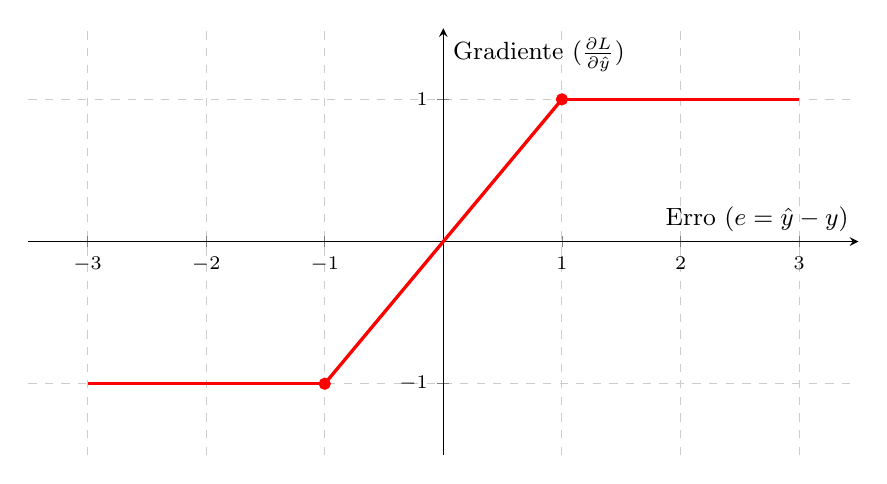
\begin{tikzpicture}
            \begin{axis}[
                % Dimensões ajustadas para caber lado a lado
                width=\linewidth, 
                height=7cm,
                xlabel={Erro ($e = \hat{y} - y$)},
                ylabel={Gradiente ($\frac{\partial L}{\partial \hat{y}}$)},
                axis lines=middle,
                grid=major,
                grid style={dashed, gray!40},
                xmin=-3.5, xmax=3.5,      % Limites do gráfico (além de delta)
                ymin=-1.5, ymax=1.5,      % Limites (um pouco além de -delta e +delta)
                ytick={-1, 0, 1},         % Ticks em -delta, 0, +delta
                xtick={-3, -2, -1, 0, 1, 2, 3}, % Ticks incluindo -delta e +delta
                legend pos=north west,
                title style={font=\bfseries\small},
                label style={font=\small},
                tick label style={font=\scriptsize}
            ]
                % Parte constante negativa (e < -delta)
                \addplot[
                    domain=-3:-1, 
                    samples=10, 
                    color=red, 
                    very thick
                ] {-1}; % Valor -delta

                % Parte linear (e entre -delta e +delta)
                \addplot[
                    domain=-1:1, 
                    samples=10, 
                    color=red, 
                    very thick
                ] {x}; % Valor e

                % Parte constante positiva (e > delta)
                \addplot[
                    domain=1:3, 
                    samples=10, 
                    color=red, 
                    very thick
                ] {1}; % Valor +delta
                
                % Pontos sólidos para os "kinks" (onde a derivada é contínua, mas não suave)
                \addplot[only marks, mark=*, color=red, mark size=2pt] coordinates {(-1,-1) (1,1)};
            \end{axis}
        \end{tikzpicture}
        \caption{Visão 2D (Gradiente vs. Erro).}%
        \label{fig:huber-derivada-2d}
    \end{subfigure}
    \hfill 
    \begin{subfigure}[b]{0.48\textwidth}
        \centering
        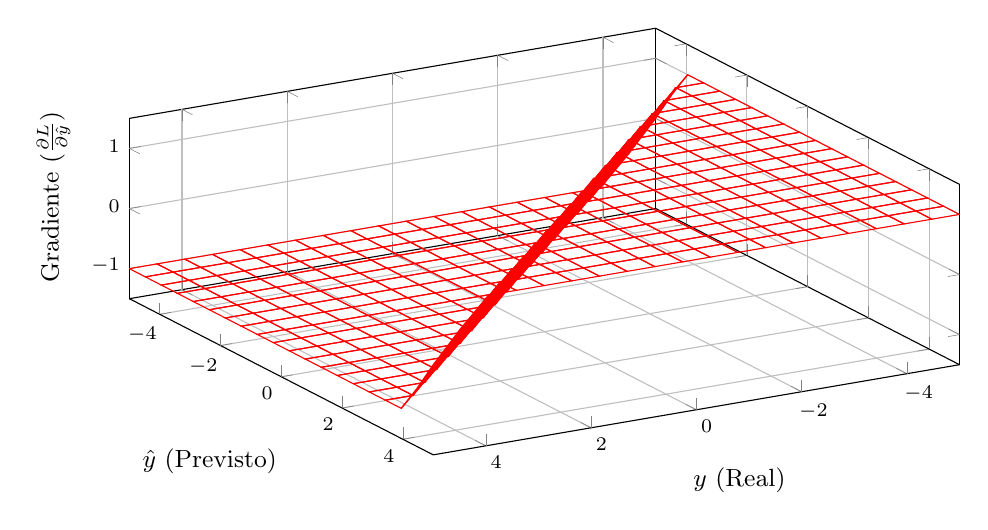
\begin{tikzpicture}
            \begin{axis}[
                % Dimensões consistentes com o gráfico (a)
                width=\linewidth,
                height=7cm,
                xlabel={$y$ (Real)},
                ylabel={$\hat{y}$ (Previsto)},
                zlabel={Gradiente ($\frac{\partial L}{\partial \hat{y}}$)},
                grid=major,
                view={150}{45}, % Mesmo ângulo de visão do seu template
                zmin=-1.5, zmax=1.5, % Espelha o eixo Y do gráfico 2D
                ztick={-1, 0, 1}, % Consistente com o 2D
                title style={font=\bfseries\small},
                label style={font=\small},
                tick label style={font=\scriptsize}
            ]
                % Gráfico da superfície do gradiente: (y_hat - y) se |erro| <= delta, senão delta*sign(erro)
                \addplot3[
                    mesh, 
                    color=red,    % Cor consistente com o gráfico 2D
                    shader=interp, 
                    domain=-5:5,    % Mesmo domínio do seu template
                    domain y=-5:5,  % Mesmo domínio do seu template
                    samples=20,     % Aumentei um pouco os samples para definir melhor a parte linear
                    % PGFPlots usa 'x' para o primeiro domain e 'y' para o segundo
                    % e = y - x  (ou seja, y_previsto - y_real)
                    % delta = 1.0
                ] { ( abs(y-x) <= 1 ? (y-x) : (1 * sign(y-x)) ) }; 
            \end{axis}
        \end{tikzpicture}
        \caption{Superfície 3D completa.}%
        \label{fig:huber-derivada-3d}
    \end{subfigure}

    \caption{Visualizações da derivada (gradiente) da função de perda Huber (com $\delta = 1.0$).}%
    \label{fig:huber-derivada}
    \fonte{O autor (2025).}
\end{figure}

Perceba que dá para ver como os pontos de descontinuidade atrapalham o formato do gráfico. Note que existem dois pontos que formam um ``bico'', eles são justamente os pontos em que $y - \hat{y} = \delta$. A descontinuidade pode não atrapalhar a plotagem do gráfico de forma geral, contudo, é sempre importante destacar os detalhes em que esses pontos refletem no gráfico da derivada.

\medskip
\begin{center}
 * * *
\end{center}
\medskip

Criada por Huber como intuito de ser utilizada para fazer uma estimação robusta de parâmetros, a perda de Huber provou ser muito mais que uma solução isolada para resolver um problema específico. E com o passar do tempo, foi tornando-se uma excelente alternativa para ser utilizada ao construir modelos de aprendizado de máquina, servindo como uma função de perda para poder medir o erro do modelo que estaca sendo treinado.

Essa seção busca listar alguns trabalhos que fazem uso dessa função de perda para resolver problemas variados no contexto de inteligência artificial.

Dito isso, vale citar os trabalhos:

\textbf{Algumas Aplicações da Perda de Huber em Problemas de Regressão}%
\index{Aplicações práticas! Perda de Huber}
\vspace{1em}

\begin{itemize}
    \item \textbf{Previsão de custos (Saúde):} Em \textit{A Huber loss-based super learner with applications to healthcare expenditures}, \textcite{HuberLossSuperLearner} desenvolvem um algoritmo de \textit{ensemble} chamado de \textit{Super Leaner} que tem como um dos objetivos fazer a previsão de custos para a área da saúde. Para isso, os autores usam uma série de outros métodos para compor o \textit{Super Leaner}, como máquinas de vetores de suporte e florestas aleatórias, além disso, para calcular a perda é feito uso da perda de Huber \parencite{HuberLossSuperLearner};
    \item \textbf{Visão computacional de veículos autônomos (Automotiva):} Além disso, no trabalho \textit{Robust Aleatoric Modeling for Future Vehicle Localization},\textcite{RobustAleatoricModelingVehicleLocalization} apresentam uma rede \textit{feedforward} para previsão robusta para fazer a localização de objetos com intuito de ser utilizada em veículos autônomos. Para fazer isso, os autores adotam a perda de Huber como função de perda para o modelo, como justificativa, eles explicam que ela apresenta a capacidade de treinar modelos de forma robusta contra caixas delimitadoras de referência (\textit{ground-truth}) anormais ou discrepantes;
    \item \textbf{Filtragem de tendências (Área):} Já no texto \textit{RobustTrend: A Huber Loss with a Combined First and Second Order Difference Regularization for Time Series Trend Filtering}, \textcite{RobustTrendHuberLoss} discutem um novo algoritmo de filtragem de tendências em séries temporais, de forma que o objetivo é extrair o sinal de tendência de uma série temporal mesmo quando houver \textit{outliers} ou variações abruptas na tendência. Com esse objetivo em mente, os autores utilizam a perda de Huber como a função de perda escolhida para ser otimizada \parencite{RobustTrendHuberLoss}. A escolha da perda de Huber é ideal para esse tipo de problema, dado que como os autores explicam, existe a presença de \textit{outliers} nos dados que estão sendo analisados;
    \item \textbf{Aplicação 4 (Área):} Por vim, vale citar o artigo \textit{Adaptive Huber Regression} dos pesquisadores \textcite{AdaptiveHuberRegression}, nele, é proposta uma mudança no parâmetro de robustificação da perda de Huber, o qual antes era fixo e agora passa a ser variável, considerando o tamanho da amostra, dimensão dos dados e outros parâmetros. Para testar essa nova forma de lidar com a perda de Huber, os autores utilizam o \textit{dataset} NCI-60, o qual possui 60 linhas de células de câncer humano \parencite{AdaptiveHuberRegression}.
\end{itemize}

\medskip
\begin{center}
 * * *
\end{center}
\medskip

Com isso, foi possível ver que a perda de Huber é uma excelente alternativa para os casos em que deseja-se controlar os pontos em que o cálculo da perda deve atuar de forma severa (usando termos quadráticos, semelhante a perda L2) e a partir de quis casos esse cálculo pode ser menos punitivo (usando termos lineares, semelhante a perda L1). Contudo, foi visto que ela tem um problema, os pontos em que essas funções se juntam gera uma descontinuidade, atrapalhando a derivação dessas funções. Para resolver esse problema da descontinuidade, pode ser utilizada como alternativa a perda Log-Cosh, a qual será vista em seguida.

\subsection{Perda Log-Cosh (Log-Cosh Loss)}%
\index{Funções de Perda!Perda Log-Cosh (Log-Cosh Loss)}%
\label{sec:log-cosh-loss}

A perda Log-Cosh é uma função de perda que vem ganhando popularidade entre os desenvolvedores, em \textit{Statistical Properties of the log-cosh Loss Function Used in Machine Learning}, \textcite{StatisticalPropetiesLogCosh} explicam que ela aparece em cenários de \textit{autoencoders} variacionais, detecção de câncer, algoritmos de aprendizado baseados em árvores (como o XGBoost) e também em regressão quantílica (\textit{quantile regression}).

Com relação a sua fórmula, é possível vê-la na Equação~\ref{eq:log-cosh-loss}. Note que ela não adiciona nenhuma função nova, ela apenas faz a aplicação da função logaritmo que recebe como parâmetro de entrada a função cosseno hiperbólica. Essa combinação gera uma séries de propriedades interessantes, as quais serão discutidas depois de analisar o seu gráfico.

\begin{equacaodestaque}{Perda Log-Cosh (\textit{Log-Cosh Loss})}
    \Loss_{\text{Log-Cosh}} (y_j, \hat{y}_j) = \sum_{j=1}^{N} \log(\cosh(y_j -\hat{y}_j))%
    \label{eq:log-cosh-loss}
\end{equacaodestaque}

Em que:

\begin{itemize}
    \item $y_j$ representa o valor real da j-ésima amostra;
    \item $\hat{y}_j$ representa o valor predito pelo modelo;
    \item $N$ representa o número de amostras.
\end{itemize}

Já com relação ao gráfico dessa função, ele está presente na Figura~\ref{fig:log-cosh-loss}. Note que a perda log-cosh atua de forma parecida com a perda de Huber. Para valores em que a diferença da saída do modelo e o rótulo real ($y_j - \hat{y}_j$) é pequena, ela tem um comportamento que lembra ao de uma função quadrática (como o \textit{MSE}). Além disso, conforme o resultado dessa diferença de valores aumenta, a perda log-cosh passa a assumir um comportamento parecido com o de uma função linear (como o \textit{MAE}). Em testes realizados por \textcite{StatisticalPropetiesLogCosh}, a perda log-cosh foi comparada com a perda de Huber, e foi verificado que as estimativas dessas funções bem como os erros padrões apresentam resultados similares. Com isso, ela pode ser uma alternativa a ser considerada caso sejam encontrados problemas ao utilizar a \textit{Huber Loss}, mas ainda é desejável manter a variação no cálculo do erro do modelo.

\begin{figure}[h!]
    \centering 

    \begin{subfigure}[b]{0.48\textwidth}
        \centering
        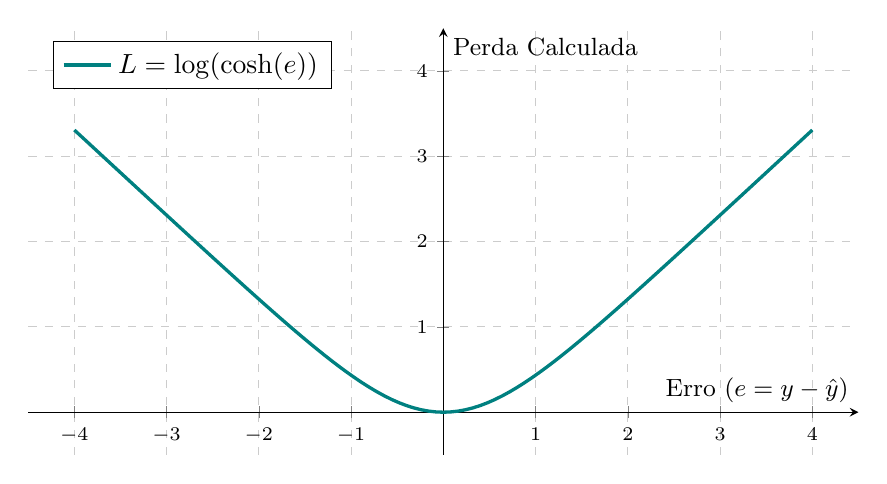
\begin{tikzpicture}
            \begin{axis}[
                % Dimensões ajustadas para caber lado a lado
                width=\linewidth,  
                height=7cm,
                xlabel={Erro ($e = y - \hat{y}$)},
                ylabel={Perda Calculada},
                axis lines=middle,
                grid=major,
                grid style={dashed, gray!40},
                xmin=-4.5, xmax=4.5,        % Limites do seu gráfico
                ymin=-0.5, ymax=4.5,         % Limites do seu gráfico
                legend pos=north west,
                title style={font=\bfseries\small},
                label style={font=\small},
                tick label style={font=\scriptsize}
            ]
                % Gráfico da função ln(cosh(x))
                \addplot[
                    domain=-4:4, 
                    samples=101,
                    color=teal, 
                    very thick
                ] {ln(cosh(x))};
                
                \addlegendentry{$L = \log(\cosh(e))$}
            \end{axis}
        \end{tikzpicture}
        \caption{Representação gráfica em duas dimensões.}%
        \label{fig:log-cosh-2d}
    \end{subfigure}
    \hfill 
    \begin{subfigure}[b]{0.48\textwidth}
        \centering
        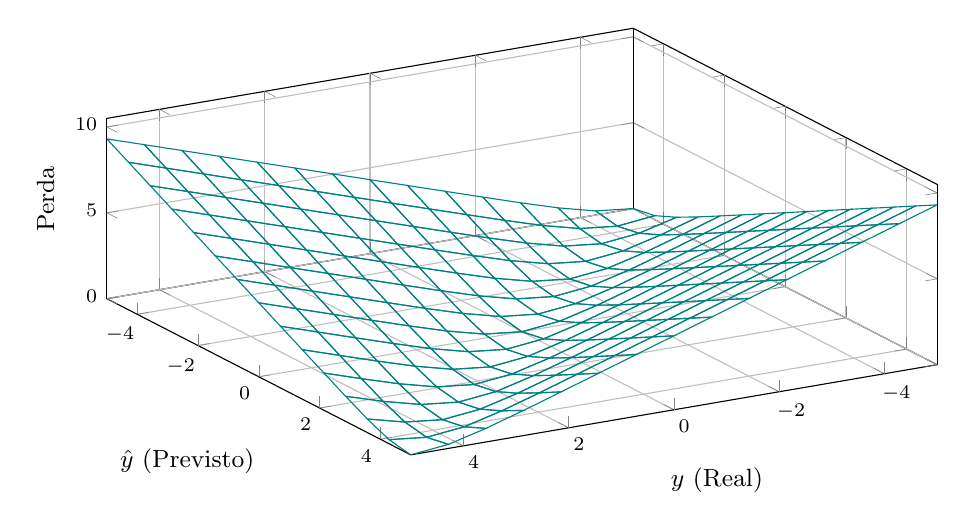
\begin{tikzpicture}
            \begin{axis}[
                % Dimensões consistentes com o gráfico (a)
                width=\linewidth,
                height=7cm,
                xlabel={$y$ (Real)},
                ylabel={$\hat{y}$ (Previsto)},
                zlabel={Perda},
                grid=major,
                view={150}{45}, % Mesmo ângulo de visão do seu template
                zmin=0, zmax=10.5, % Limite Z ajustado para Log-Cosh com domínio -5:5
                title style={font=\bfseries\small},
                label style={font=\small},
                tick label style={font=\scriptsize}
            ]
                % Gráfico da superfície da Log-Cosh Loss
                \addplot3[
                    mesh,           
                    color=teal,     % Cor consistente com o gráfico 2D
                    shader=interp,  
                    domain=-5:5,    % Mesmo domínio do seu template
                    domain y=-5:5,  % Mesmo domínio do seu template
                    samples=15      % Mesma resolução da malha
                ] { ln(cosh(x - y)) }; % A função Log-Cosh 3D
            \end{axis}
        \end{tikzpicture}
        \caption{Representação gráfica em três dimensões.}%
        \label{fig:log-cosh-3d}
    \end{subfigure}

    % --- Legenda e Fonte da Figura Principal ---
    \caption{Visualizações da função de perda Log-Cosh (\textit{Log-Cosh Loss}) em duas e em três dimensões.}%
    \label{fig:log-cosh-loss}
    \fonte{O autor (2025).}
\end{figure}

\medskip
\begin{center}
 * * *
\end{center}
\medskip

\textbf{Características da Perda Log-Cosh}
\vspace{1em}

Seguindo adiante, é possível discutir agora algumas das propriedades dessa função de perda. As quais estão apresentas a seguir.

\begin{itemize}
    \item \textbf{Convexa:} É possível ver pelo gráfico da Figura~\ref{fig:log-cosh-loss} que ela é uma função convexa, apresentando um formato característico de funil, além de possuir um único ponto de mínimo global. Mas note que não é possível garantir essa propriedade em cenários em que ela está sendo aplicada em modelos de redes neurais densas, devido as transformações não-lineares que ocorrem;
    \item \textbf{Robustez para \textit{outliers}:} Assim como a perda de Huber e o erro absoluto médio, a perda log-cosh não pune de forma agressiva os erros cometidos pelo modelo ao ser treinado. Isso garante que essa função possa ser aplicada em cenários em que os dados possuem muitos \textit{outliers} sem afetar drasticamente o treinamento do modelo;
    \item \textbf{Continuidade e diferenciabilidade:} Diferente de a perda de Huber, que possui pontos de descontinuidade na ligação da função linear com a quadrática, a perda log-cosh consegue ser contínua em todos os seus pontos. Além disso, isso também é uma vantagem sobre o erro absoluto médio, pois este também apresenta um ponto de descontinuidade em 0, o qual precisa do cálculo do subgradiente para garantir o aprendizado dos modelos que fazem uso de otimizadores baseados em gradiente. Dessa forma, além de ser contínua, a perda log-cosh pode ser derivada em todos os seus pontos, algo útil caso esteja sendo usados otimizadores que atuam com o uso do cálculo do gradiente.
\end{itemize}

\medskip
\begin{center}
 * * *
\end{center}
\medskip

Visto essas diferentes propriedades dessa função, cabe agora analisar a sua derivada, a qual será útil para a retropropagação e consequentemente o aprendizado do modelo. Para isso, ela pode ser vista na Equação~\ref{eq:log-cosh-derivada}. Perceba que a derivada da perda log-cosh envolve o cálculo da tangente hiperbólica, que coincidentemente, também é utilizada em aprendizado de máquina como uma função de ativação, tendo como objetivo introduzir a não-linearidade para as saídas de uma camada densa.

\begin{equacaodestaque}{Derivada Parcial da Perda Log-Cosh em Relação a $\hat{y}_j$}
    \frac{\partial\Loss_{\text{Log-Cosh}}}{\partial\hat{y}_j} = \tanh(\hat{y}_j - y_j)%
    \label{eq:log-cosh-derivada}
\end{equacaodestaque}

Tendo a fórmula da sua derivada, o próximo passo é analisar o seu gráfico, o qual está representado na Figura~\ref{eq:log-cosh-derivada}. Caso você leitor tenha lido o Capítulo~\ref{cap:ativacao-sigmoidais}, você não verá nada novo aqui, é apenas o gráfico característico em formato de ``S'' que as funções sigmoidais possuem. Um ponto interessante a ser destacado ao analisar a figura é que as saídas dessa função serão em um intervalo $[-1, 1]$, o que podem fazer com que o sinal do gradiente fique alternando, garantindo uma convergência mais rápida em alguns casos.

\begin{figure}[h!]
    \centering
    \begin{subfigure}[b]{0.48\textwidth}
        \centering
        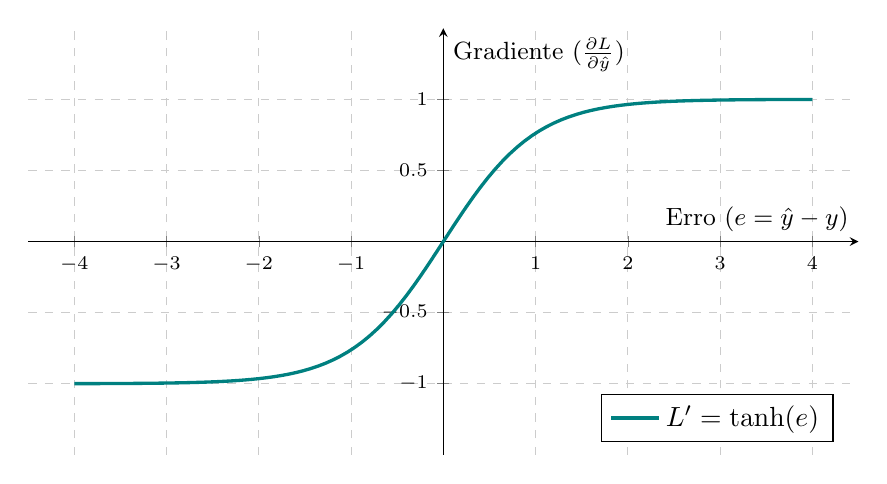
\begin{tikzpicture}
            \begin{axis}[
                % Dimensões ajustadas para caber lado a lado
                width=\linewidth,  
                height=7cm,
                xlabel={Erro ($e = \hat{y} - y$)},
                ylabel={Gradiente ($\frac{\partial L}{\partial \hat{y}}$)},
                axis lines=middle,
                grid=major,
                grid style={dashed, gray!40},
                xmin=-4.5, xmax=4.5,        % Limites do seu gráfico
                ymin=-1.5, ymax=1.5,         % Limites do seu gráfico
                ytick={-1, -0.5, 0, 0.5, 1}, % Marcas no eixo y
                legend pos=south east,
                title style={font=\bfseries\small},
                label style={font=\small},
                tick label style={font=\scriptsize}
            ]
                % Gráfico da função tanh(x)
                \addplot[
                    domain=-4:4, 
                    samples=101,
                    color=teal, 
                    very thick
                ] {tanh(x)};
                
                \addlegendentry{$L' = \tanh(e)$}
            \end{axis}
        \end{tikzpicture}
        \caption{Visão 2D (Gradiente vs. Erro).}%
        \label{fig:log-cosh-derivada-2d}
    \end{subfigure}
    \hfill 
    \begin{subfigure}[b]{0.48\textwidth}
        \centering
        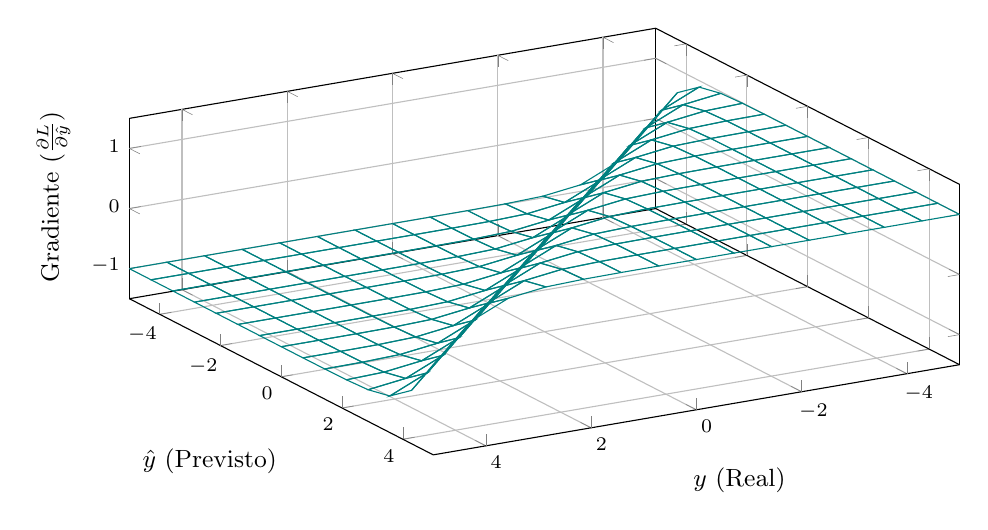
\begin{tikzpicture}
            \begin{axis}[
                % Dimensões consistentes com o gráfico (a)
                width=\linewidth,
                height=7cm,
                xlabel={$y$ (Real)},
                ylabel={$\hat{y}$ (Previsto)},
                zlabel={Gradiente ($\frac{\partial L}{\partial \hat{y}}$)},
                grid=major,
                view={150}{45}, % Mesmo ângulo de visão do seu template
                zmin=-1.5, zmax=1.5, % Espelha o eixo Y do gráfico 2D
                ztick={-1, 0, 1}, % Consistente com o 2D
                title style={font=\bfseries\small},
                label style={font=\small},
                tick label style={font=\scriptsize}
            ]
                % Gráfico da superfície do gradiente: tanh(y_hat - y)
                \addplot3[
                    mesh,           
                    color=teal,     % Cor consistente com o gráfico 2D
                    shader=interp,  
                    domain=-5:5,    % Mesmo domínio do seu template
                    domain y=-5:5,  % Mesmo domínio do seu template
                    samples=15      % Mesma resolução da malha
                ] { tanh(y - x) }; % A função da derivada: tanh(y_previsto - y_real)
            \end{axis}
        \end{tikzpicture}
        \caption{Superfície 3D completa.}%
        \label{fig:log-cosh-derivada-3d}
    \end{subfigure}

    \caption{Visualizações da derivada (gradiente) da função de perda Log-Cosh.}%
    \label{fig:log-cosh-derivada}
    \fonte{O autor (2025).}
\end{figure}

\medskip
\begin{center}
 * * *
\end{center}
\medskip

Além das aplicações discutidas no início da seção sobre a perda Log-cosh, ela também está presente em várias outras pesquisas. Para isso, essa seção busca citar algumas aplicações dessa função de perda para resolver problemas no contexto de aprendizado de máquina.

Dito isso vale citar os trabalhos:

\textbf{Algumas Aplicações da Perda Log-Cosh em Problemas de Regressão}%
\index{Aplicações práticas! Perda Log-Cosh}
\vspace{1em}

\begin{itemize}
    \item \textbf{Previsão de índices do mercado financeiro (Economia):} Em \textit{Financial Market Forecasting using RNN, LSTM, BiLSTM, GRU and Transformer-Based Deep Learning Algorithms}, \textcite{FinantialMarketForecastingUsingRNN} estavam criando algoritmos de aprendizado de máquina para fazer a previsão de índices de ações globais (como o FTSE 100, S\&P 500 e HSI), para isso, eles constroem diferentes modelos, como uma rede neural recorrente. Além disso, eles utilizam diversas funções como métricas para avaliar os modelos construídos, Log-Cosh é uma dessas funções, junto com o erro absoluto médio (\textit{MAE}), erro quadrático médio (\textit{MSE}), a raiz do erro quadrático médio (\textit{RMSE}) e também a perda de Huber \parencite{FinantialMarketForecastingUsingRNN};
    \item \textbf{Predição de bioatividade em moléculas (Farmácia):} Já em \textit{Siamese Recurrent Neural Network with a Self-Attention Mechanism for Bioactivity Prediction} \textcite{SiameseRecurrentNeuralNetwork} apresentam uma rede neural recorrente (\textit{RNN}) siamesa com o intuito de fazer a predição da biotividade de pequenas moléculas, um procedimento muito útil na descoberta de remédios. Os autores argumentam que a perda Log-Cosh foi uma função de perda ideal para ser aplicada nesse problema, pois apresentou o melhor desempenho das perdas que foram testadas: perda constrativa (\textit{constractive loss}), perda de Huber, perda L1 e perda L2 \parencite{SiameseRecurrentNeuralNetwork};
    \item \textbf{Aplicação 3 (Área):} Por fim, no trabalho \textit{An Effective Method for Detecting Unknown Types of Attacks Based on Log-Cosh Variational Autoencoder}, \textcite{AnEffectiveMethodForDetectingUnknowTypes} propõem um modelo de \textit{deep learning} chamado de \textit{LVAE (Log-Cosh Variational Autoencoder)} com intuito detectar tipos desconhecidos de ataques em redes. A perda log-cosh é utilizada no modelo como a função de perda de reconstrução dentro do modelo \textit{variational autoencoder} \parencite{AnEffectiveMethodForDetectingUnknowTypes}.
\end{itemize}

\medskip
\begin{center}
 * * *
\end{center}
\medskip

Vistas essas quatro funções: O erro quadrático médio (\textit{MSE}), o erro absoluto médio (\textit{MAE}), a perda de Huber e a perda log-cosh. Já é possível resolver a grande maioria dos problemas de regressão em aprendizado de máquina. Contudo, existem problemas que vão além dessas perdas, precisando de funções mais específicas para garantir uma melhor avaliação do erro e a partir dele, saber atualizar o gradiente e com isso o modelo aprender de fato.

Para isso, as próximas seções buscam explorar diferentes cenários em que as funções de perda para regressão vistas até agora não são a melhor escolha. Assim, serão exploradas mais três seções, a primeira focada no erro relativo, a segunda focada em funções de erro que não calculam a média dos diversos erros, e a última para casos em são utilizas distribuições específicas para os valores.

\section{Lidando com a Escala: Foco no Erro Relativo}

As funções de perda vistas até agora possuem um detalhe em comum: todas lidam com o erro de fazendo um cálculo absoluto. Para entender melhor essa frase é possível ilustrar isso com um exemplo. Considere que existem duas situações que está sendo previsto os valores de imóveis:

\begin{itemize}
    \item Cenário A: O modelo previu que uma casa vale 50.000 R\$, enquanto no rótulo está que ela vale 100.000 R\$;
    \item Cenário B: O modelo previu que uma casa vale 950.000 R\$, enquanto no rótulo está que ela vale 1.000.000 R\$.
\end{itemize}

Para fazer o trabalho dessa regressão foi utilizada a função de perda erro quadrático médio. Note que essa função calcula primeiro a diferença entre o valor previsto pelo modelo e o valor apresentado no rótulo. Com isso, essa diferença será a mesma para esses dois cenários, 50.000 R\$.

Essa é uma forma de analisar o problema. Mas também pode ser visto de forma relativa, veja que o modelo do cenário A previu que a casa vale apenas a metade do seu valor real, ele fez uma previsão subestimada. Por outro lado, o modelo do cenário B foi mais realista, ele sabe que a casa possui um valor alto, contudo, ainda sim ficou uma distância do valor real. 

O erro quadrático médio, e as outras três funções de perda vistas até agora tratam os erros dos cenários A e B como iguais. Mas e se você estivesse em uma situação em que o modelo subestimar os valores dos rótulos seja considerada muito negativa, e por isso deve ser evitada?

Para isso, essa seção busca explicar a função de perda erro quadrático médio logarítmico, que possui uma tendência de penalizar mais as subestimação. Serão vistos seus gráficos, sua fórmula e aplicações, assim como nas outras funções vistas até o momento.

\subsection{Erro Quadrático Médio Logarítmico (MSLE)}%
\index{Funções de Perda!Erro Quadrático Médio Logarítimico (MSLE)}%

A primeira função a ser vista nessa nova categoria é o erro quadrático médio logarítmico, também chamado de \textit{Mean Squared Logarithmic Error} (\textit{MSLE}). A sua fórmula é dada pela Equação~\ref{eq:msle-loss}. Perceba que diferente das funções vistas até agora, ela faz o cálculo do logaritmo natural dos valores reais ($y_j$) e dos valores previstos pelo modelo ($\hat{y}_j$). Além disso, um ponto que vale a pena ser destacado é com relação ao valor de 1 que é somado aos valores antes do cálculo do logaritmo. Isso ocorre para evitar com que esse resultado possa ser negativo ou zero, gerando uma indeterminação ao calcular o logaritmo.

\begin{equacaodestaque}{Erro Quadrático Médio Logarítmico (\textit{MSLE})}
    \Loss_{\text{MSLE}} (y_j, \hat{y}_j) = \frac{1}{N} \sum_{j=1}^{N} (\ln(y_j + 1) -\ln(\hat{y}_j + 1))^2%
    \label{eq:msle-loss}
\end{equacaodestaque}

Em que:

\begin{itemize}
    \item $y_j$ representa o valor real da j-ésima amostra;
    \item $\hat{y}_j$ representa o valor predito pelo modelo;
    \item $N$ representa o número de amostras.
\end{itemize}

Com relação ao seu gráfico, ele pode visto na Figura~\ref{fig:msle-loss}. Na Figura~\ref{fig:msle-2d}, à esquerda, está a visão em duas dimensões dessa função, enquanto na Figura~\ref{fig:msle-3d}, à direita, está a visão em três dimensões. Perceba que a adição do logaritmo para essa função traz alguns benefícios como a continuidade em seus pontos além de garantir uma superfície suave e diferenciável. Contudo, a principal característica dessa função é que ela é uma função assimétrica com relação ao eixo $y$ e por consequência, ela apresenta uma tendência de penalizar mais as subestimações feitas pelo modelo.

\begin{figure}[h!]
    \centering 

    \begin{subfigure}[b]{0.48\textwidth}
        \centering
        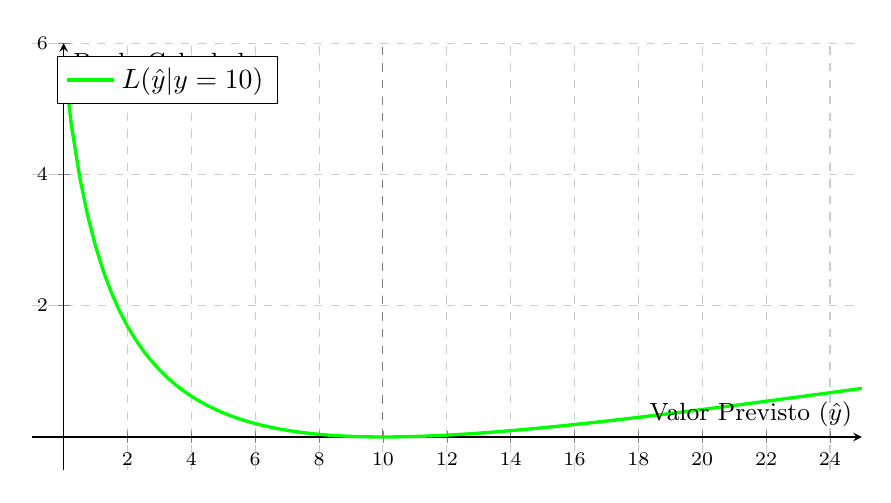
\begin{tikzpicture}
            \begin{axis}[
                % Dimensões ajustadas para caber lado a lado
                width=\linewidth,  
                height=7cm,
                xlabel={Valor Previsto ($\hat{y}$)},
                ylabel={Perda Calculada},
                axis lines=middle,
                grid=major,
                grid style={dashed, gray!40},
                xmin=-1, xmax=25,        % Limites do seu gráfico
                ymin=-0.5, ymax=6,         % Limites do seu gráfico
                legend pos=north west,
                title style={font=\bfseries\small},
                label style={font=\small},
                tick label style={font=\scriptsize}
            ]
                % Gráfico da função (ln(11) - ln(x+1))^2
                \addplot[
                    domain=0:25, 
                    samples=101,
                    color=green, 
                    very thick
                ] {(ln(10+1) - ln(x+1))^2};
                
                \addlegendentry{$L(\hat{y} | y=10)$}

                % Linha vertical para marcar o valor real
                \draw[dashed, gray] (axis cs:10, 0) -- (axis cs:10, 6);
                \node[above, gray!80, font=\tiny] at (axis cs:10, 6) {Valor Real ($y=10$)};
            \end{axis}
        \end{tikzpicture}
        \caption{Visão 2D (corte em $y=10$).}%
        \label{fig:msle-2d}
    \end{subfigure}
    \hfill 
    \begin{subfigure}[b]{0.48\textwidth}
        \centering
        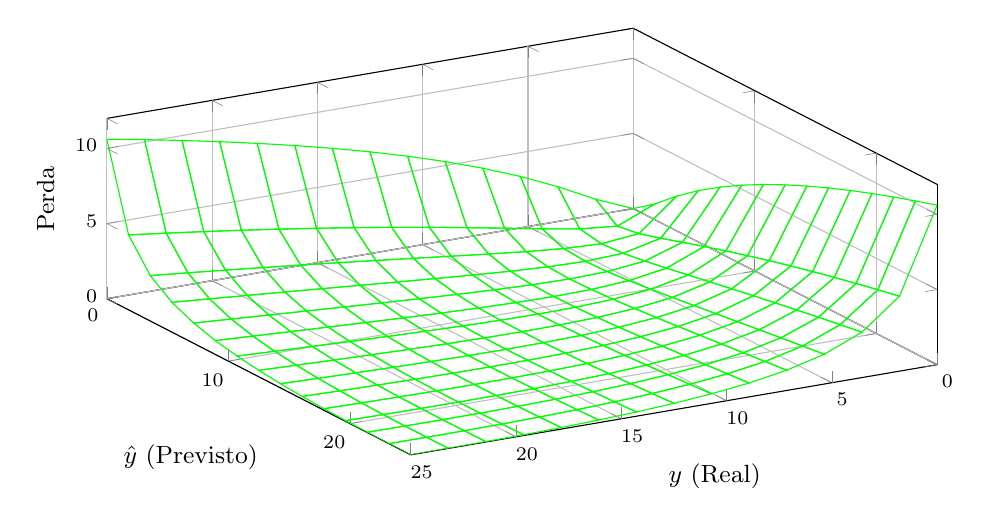
\begin{tikzpicture}
            \begin{axis}[
                % Dimensões consistentes com o gráfico (a)
                width=\linewidth,
                height=7cm,
                xlabel={$y$ (Real)},
                ylabel={$\hat{y}$ (Previsto)},
                zlabel={Perda},
                grid=major,
                view={150}{45}, % Mesmo ângulo de visão do seu template
                zmin=0, zmax=12, % Ajustado para (ln(26)-ln(1))^2
                title style={font=\bfseries\small},
                label style={font=\small},
                tick label style={font=\scriptsize}
            ]
                % Gráfico da superfície da MSLE
                \addplot3[
                    mesh,           
                    color=green,    % Cor consistente com o gráfico 2D
                    shader=interp,  
                    domain=0:25,    % Domínio > -1 (usando 0:25)
                    domain y=0:25,  % Domínio > -1 (usando 0:25)
                    samples=15      % Mesma resolução da malha
                ] { (ln(x+1) - ln(y+1))^2 }; % A função MSLE 3D
            \end{axis}
        \end{tikzpicture}
        \caption{Superfície 3D completa.}%
        \label{fig:msle-3d}
    \end{subfigure}

    \caption{Visualizações da função de perda MSLE (\textit{Mean Squared Logarithmic Error}).}%
    \label{fig:msle-loss}
    \fonte{O autor (2025).}
\end{figure}

\medskip
\begin{center}
 * * *
\end{center}
\medskip

\textbf{Características do Erro Quadrático Médio Logarítmico}
\vspace{1em}

Conhecendo a fórmula dessa função e suas representações gráficas, cabe agora discutir algumas das características dessa função:

\begin{itemize}
    \item \textbf{Foco no erro relativo (Percentual):} Quando o \textit{MSLE} é utilizado como função de perda, diferente das outras vistas até agora que medem o erro absoluto, o erro quadrático logarítmico médio mede o erro percentual/relativo. Isso acontece por conta dos uso dos logaritmos dessa função, que são responsáveis por comprimir a escala dos dados. Com isso, erros em que o valor predito é 50\% menor que o real são mais penalizados em que cenários nos quais o valor predito é 5\% menor;
    \item \textbf{Tendência de penalizar subestimações:} Como pode ser visto nos gráficos da Figura~\ref{fig:msle-loss}, a função \textit{MSLE} não forma uma curva convexa simétrica verticalmente, perceba que conforme os valores vão diminuindo, a perda aumenta consideravelmente. Enquanto isso, conforme os valores aumentam, a perda também aumenta, mas não de forma tão agressiva quanto no sentido inverso. Isso significa que quanto maior for a diferença entre o valor previsto $\hat{y}_j$ e o valor real $y_j$, existe uma tendência de que a perda será maior;
    \item \textbf{Continuidade e Diferenciabilidade:} Ainda com relação aos seus gráficos é possível analisar a continuidade dessa função. Note que ela não apresenta nenhum ponto ``problema'' que poderia afetar o cálculo das derivadas e com isso atrapalhar o fluxo do gradiente. Além disso, o uso dos logaritmos para essa função permite que suas curvas sejam suaves, o que também ajuda na sua continuidade.
\end{itemize}

\medskip
\begin{center}
 * * *
\end{center}
\medskip

Cabe também discutir as derivadas do \textit{MSLE}, as quais serão úteis para construir o vetor gradiente do erro. Na equação~\ref{eq:msle-derivada} está a derivada do erro quadrático médio logarítmico em relação os valores preditos pelo modelo $\hat{y}_j$

\begin{equacaodestaque}{Derivada Parcial do Erro Quadrático Médio Logarítmico (\textit{MSLE}) em Relação a $\hat{y}_j$}
    \frac{\partial\Loss_{\text{MSLE}}}{\partial\hat{y}_j} (y_j, \hat{y}_j) = -\frac{2}{N} \cdot \frac{\ln(y_j + 1) -\ln(\hat{y}_j + 1)}{\hat{y}_j + 1}%
    \label{eq:msle-derivada}
\end{equacaodestaque}

Em seguida, é possível ver representação gráfica da derivada da Equação~\ref{eq:msle-derivada} na Figura~\ref{fig:msle-derivada}. Seguindo a mesma regra das outras figuras apresentadas até agora, na Figura~\ref{fig:msle-derivada-2d}, à esquerda, está a representação em duas dimensões, enquanto na Figura~\ref{fig:msle-derivada-3d}, à direita, está a representação da superfície no espaço.

\begin{figure}[h!]
    \centering 

    \begin{subfigure}[b]{0.48\textwidth}
        \centering
        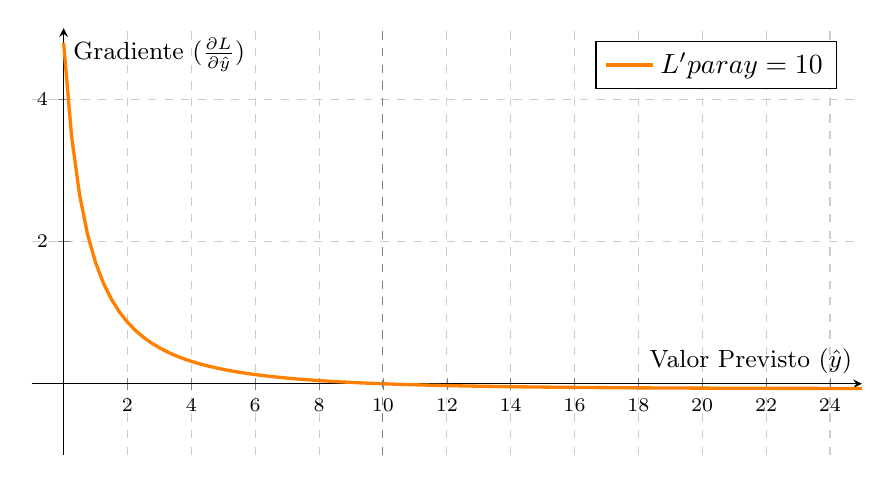
\begin{tikzpicture}
            \begin{axis}[
                % Dimensões ajustadas para caber lado a lado
                width=\linewidth,  
                height=7cm,
                xlabel={Valor Previsto ($\hat{y}$)},
                ylabel={Gradiente ($\frac{\partial L}{\partial \hat{y}}$)},
                axis lines=middle,
                grid=major,
                grid style={dashed, gray!40},
                xmin=-1, xmax=25,        % Limites do seu gráfico
                ymin=-1, ymax=5,         % Limites do seu gráfico
                legend pos=north east,
                title style={font=\bfseries\small},
                label style={font=\small},
                tick label style={font=\scriptsize}
            ]
                % Gráfico da derivada (fórmula corrigida para corresponder aos eixos)
                \addplot[
                    domain=0:25, 
                    samples=101,
                    color=orange, 
                    very thick
                ] {2 * (ln(10+1) - ln(x+1)) / (x+1)}; % Corrigido (removido o -)
                
                \addlegendentry{$L' \text{ para } y=10$}

                % Linha vertical para marcar o valor real
                \draw[dashed, gray] (axis cs:10, -1) -- (axis cs:10, 5);
                \node[above, gray!80, font=\tiny] at (axis cs:10, 5) {Valor Real};
            \end{axis}
        \end{tikzpicture}
        \caption{Visão 2D (corte em $y=10$).}%
        \label{fig:msle-derivada-2d}
    \end{subfigure}
    \hfill 
    \begin{subfigure}[b]{0.48\textwidth}
        \centering
        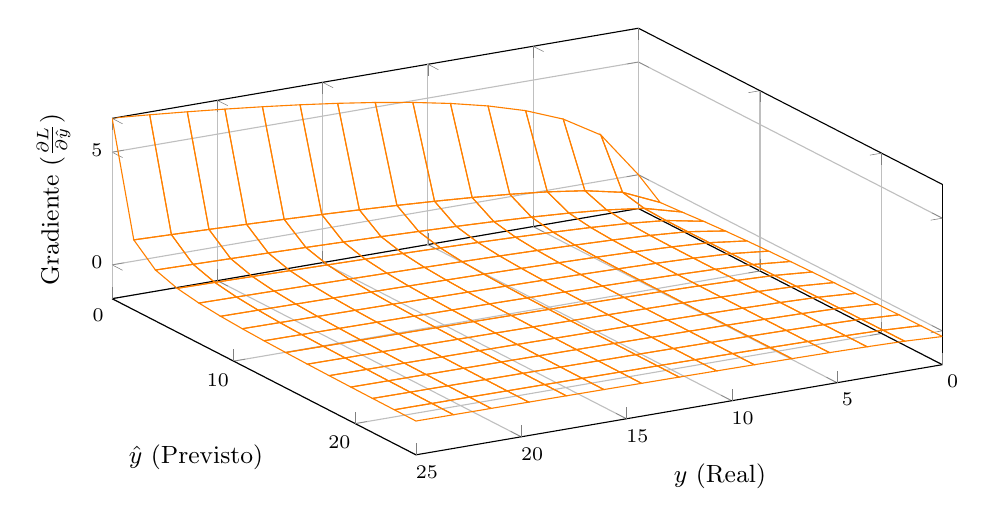
\begin{tikzpicture}
            \begin{axis}[
                % Dimensões consistentes com o gráfico (a)
                width=\linewidth,
                height=7cm,
                xlabel={$y$ (Real)},
                ylabel={$\hat{y}$ (Previsto)},
                zlabel={Gradiente ($\frac{\partial L}{\partial \hat{y}}$)},
                grid=major,
                view={150}{45}, % Mesmo ângulo de visão do seu template
                zmin=-1.5, zmax=6.5, % Ajustado para o pico do gradiente
                title style={font=\bfseries\small},
                label style={font=\small},
                tick label style={font=\scriptsize}
            ]
                % Gráfico da superfície da derivada da MSLE (fórmula corrigida)
                \addplot3[
                    mesh,           
                    color=orange,   % Cor consistente com o gráfico 2D
                    shader=interp,  
                    domain=0:25,    % Domínio de x (y_real)
                    domain y=0:25,  % Domínio de y (y_previsto)
                    samples=15      % Mesma resolução da malha
                ] { 2 * (ln(x+1) - ln(y+1)) / (y+1) }; % L' = 2(log(y+1)-log(y_hat+1))/(y_hat+1)
            \end{axis}
        \end{tikzpicture}
        \caption{Superfície 3D completa.}%
        \label{fig:msle-derivada-3d}
    \end{subfigure}

    \caption{Visualizações da derivada (gradiente) da função de perda MSLE.}%
    \label{fig:msle-derivada}
    \fonte{O autor (2025).}
\end{figure}

Perceba que o uso dos logaritmos na função, fazem com que a superfície do \textit{MSLE} tenha uma superfície suave e contínua. Isso também é refletido na sua derivada, o que é de grande utilidade para os algoritmos de otimização que trabalham com o gradiente, de forma que eles não precisam ter que escapar de pontos de descontinuidade, como ocorriam em outras funções anteriores, como a perda de Huber e o \textit{MAE}.

\medskip
\begin{center}
 * * *
\end{center}
\medskip

Além disso, voltando para o exemplo anterior dos modelos prevendo preços de imóveis, é possível agora discutir como o \textit{MSLE} se compara ao erro quadrático médio, e como ele pode ser uma alternativa para função de perda em cenários em que é preciso garantir que as subestimações sejam mais penalizadas.

Para isso, a Tabela~\ref{tab:comparativo-mse-msle} compara os dois cenários vistos na seção anterior, e mostra qual foi o valor do erro calculado para essas situações.

\begin{table}[htbp]
    \centering
    \begin{threeparttable}
        \caption{Comparativo das funções de perda \textit{MSE} e \textit{MSLE}}%
        \label{tab:comparativo-mse-msle}
        \begin{tabular}{l c c c c }
            \toprule
            Cenário & $y_j$ (real) & $\hat{y}_j$ (predito) & \textit{MSE} & \textit{MSLE} \\
            \midrule
            Cenário A & $100.000$ & $50.000$ & $2.500.000.000$ & $0,4804$ \\
            Cenário B & $1.000.000$ & $950.000$ & $2.500.000.000$ & $0,0026$ \\
            \bottomrule
        \end{tabular}
        
        \begin{tablenotes}[para] % Inicia o ambiente das notas
            \small % Define a fonte como menor, padrão ABNT para fontes
            \item[] Fonte: O autor (2025).
        \end{tablenotes}

    \end{threeparttable} % Finaliza o ambiente
\end{table}

Perceba que o erro quadrático médio só se importa com a grandeza dos valores, a nos dois cenários o erro é o mesmo, e consequentemente a atualização do gradiente será a mesma, o modelo sabe que está errado e tem que melhorar nas predições, mas para ele os erros são de mesma magnitude. Contudo, olhando agora para os valores do \textit{MSLE}, é possível ver que o cenário A, em que o modelo subestimou o valor do imóvel, é cerca de 185 vezes pior que o do cenário B. Neste caso, como no cenário A o erro foi maior, as atualizações nos parâmetros do modelo também serão maiores, enquanto no cenário B ainda irá ocorrer atualizações, mas como apontado, os valores dos parâmetros irão ter uma variação menor de uma época para a próxima.

Com isso, é possível ter uma ideia de que o erro quadrático logarítmico médio pode ser uma excelente alternativa para os casos em que as subestimações do modelo devem ser evitadas.

\medskip
\begin{center}
 * * *
\end{center}
\medskip

Além disso, assim como o erro quadrático médio, que possui uma métrica derivada, o \textit{RMSE}. Com o erro quadrático logarítmico médio não é diferente. Assim, é possível também utilizar a métrica raiz do erro quadrático médio logarítmico (\textit{RMSLE}) que serve de métrica para avaliar modelos de aprendizado de máquina. Neste caso, o \textit{RMSLE} é dado pelo cálculo da raiz quadrada da função de perda \textit{RMSE}.

\begin{equacaodestaque}{Raiz do Erro Quadrático Médio Logarítmico (\textit{RMSLE})}
    \Loss_{\text{MSLE}} (y_j, \hat{y}_j) = \sqrt{\frac{1}{N} \sum_{j=1}^{N} (\log(y_j + 1) -\log(\hat{y}_j + 1))^2}%
    \label{eq:rmsle-metric}
\end{equacaodestaque}

Em que:

\begin{itemize}
    \item $y_j$ representa o valor real da j-ésima amostra;
    \item $\hat{y}_j$ representa o valor predito pelo modelo;
    \item $N$ representa o número de amostras.
\end{itemize}

Ao calcular a raiz quadrada do erro quadrático médio logarítmico é possível ter uma noção melhor da magnitude dos erros, dado que eles são mascarados ao serem elevados ao quadrado pela expressão do \textit{RMSE}. Dessa forma, a equação da raiz do erro quadrático médio logarítmico consegue melhorar a interpretabilidade dos erros, servindo como uma métrica, a qual pode ser aplicada para problemas em que as subestimações devem ser mais penalizadas.

\medskip
\begin{center}
 * * *
\end{center}
\medskip

\textbf{Algumas Aplicações do Erro Quadrático Logarítmico Médio em Problemas de Regressão}%
\index{Aplicações práticas! Erro quadrático logarítimico médio}
\vspace{1em}

Visto o erro quadrático logarítmico médio e também o \textit{RMSLE}, cabe agora discutir alguns cenários em que essa função pode ser aplicada para resolver problemas de regressão. Você verá que essas duas funções podem aparecer tanto como métricas, avaliando o desempenho do modelo, mas também podem atuar como uma função de perda, servindo de guia para o cálculo do gradiente e consequentemente o ajuste dos parâmetros da rede.

Dito isso, vale destacar os trabalhos:

\begin{itemize}
    \item \textbf{Predição do preço de casas (Mercado imobiliário):} Em \textit{A Net Over Your Head: A Neural Network Approach to Home Price Predictions}, \textcite{SunKim-NetOverYourHead} discutem formas de prever o preço de casas, para isso eles desenvolvem uma rede neural, indo contra a tendência de utilizar técnicas mais tradicionais, como regressão linear ou florestas aleatórias. Para isso, eles utilizam como métrica o \textit{RMSLE}, como justificativa, os autores explicam que o \textit{dataset} que está sendo utilizado apresenta casas que têm ordem de magnitude de diferença de preço, e com isso uma previsão ruim para uma casa de alto valor terá mais peso que uma previsão ruim para uma casa de baixo valor; ao usar o \textit{RMSLE} é possível capturar as ordens de magnitude dos preços das casas, algo que não acontece com o \textit{RMSE} \parencite{SunKim-NetOverYourHead};
    \item \textbf{Predição no tempo de internação de pacientes (Saúde):} Além disso, no trabalho \textit{Predicting Hospital Length of Stay of Patients Leaving the Emergency Department}, \textcite{Winter2023PredictingLOS} analisam maneiras de prever o tempo de internação de um paciente qualquer após receber alta no pronto-socorro e sua transferência para a próxima unidade hospitalar. Com esse objetivo em mente, os autores usam um modelo de regressão de \textit{gradient boosting} com arquitetura \textit{CatBoost}, para a função de perda, os autores escolhem duas, a primeira sendo o \textit{RMSE} e a segunda o \textit{RMSLE}, como justificativa, os autores apontam que o \textit{RMSLE} penaliza erros proporcionais e é menos afetado por \textit{outliers};
    \item \textbf{Previsão de séries temporais (Área):} Por fim, no texto \textit{A Comprehensive Survey of Regression Based Loss Functions for Time Series Forecasting}, \textcite{Jadon2022ComprehensiveSurvey} analisam uma série de funções de perda que são comumente utilizadas na previsão de séries temporais, sendo uma delas o \textit{MSLE}. No trabalho, os autores apontam que o erro quadrático logaritmo médio reduz o efeito punitivo de diferenças significativas em grandes valores previsos; sendo apropriado quando o modelo prevê quantidades não escalonadas diretamente \parencite{Jadon2022ComprehensiveSurvey}. Além disso, \textcite{Jadon2022ComprehensiveSurvey} analisam também o \textit{RMSLE}, explicando que ele pode ser uma função de perda para ser utilizada em cenários em que a subestimação dos valores reais não é aceitável, mas a superestimações do modelo não são consideradas um problema.
\end{itemize}

\medskip
\begin{center}
 * * *
\end{center}
\medskip

Visto o erro quadrático logarítmico médio, uma função de perda assimétrica que tem como principal característica a tendência de penalizar mais as subestimações feitas pelo modelo, o próximo passo é discutir agora uma função que possua a característica contrária, de penalizar mais as superestimações. Para isso, é preciso ir para a próxima seção dessa capítulo, que analisa funções de perda que calculam a perda levando em consideração outros cálculos, além da média, e nela estudar a perda quantílica, que pode ser ajustada de forma que possa penalizar mais as subestimações ou as superestimações, dependendo de como seus parâmetros são ajustados.

\section{Mudando o Objetivo da Previsão: Além da Média}

Até agora todas as funções de perda vistas possui um detalhe em comum: elas calculavam o erro para um conjunto $m$ de instâncias, e a partir disso aplicavam o cálculo da média dos erros. Mas existem funções de perda que vão além do cálculo da média para calcular o erro de um modelo de regressão.

Ao calcular a média dos erros, está sendo presumido que a tendência central é a característica mais informativa daquela distribuição de dados, seguindo a clássica distribuição Gaussiana, mas e quando isso não for a realidade? E quando a caraterística mais comum estiver deslocada mais para à esquerda (como na Figura~\ref{fig:dist-skew-esquerda}), ou mais para à direita da distribuição (como na Figura~\ref{fig:dist-skew-direita})?

\begin{figure}[h!]
    \centering 

    % --- SUBFIGURA (a): Distribuição Assimétrica à Direita ---
    \begin{subfigure}[b]{0.48\textwidth}
        \centering
        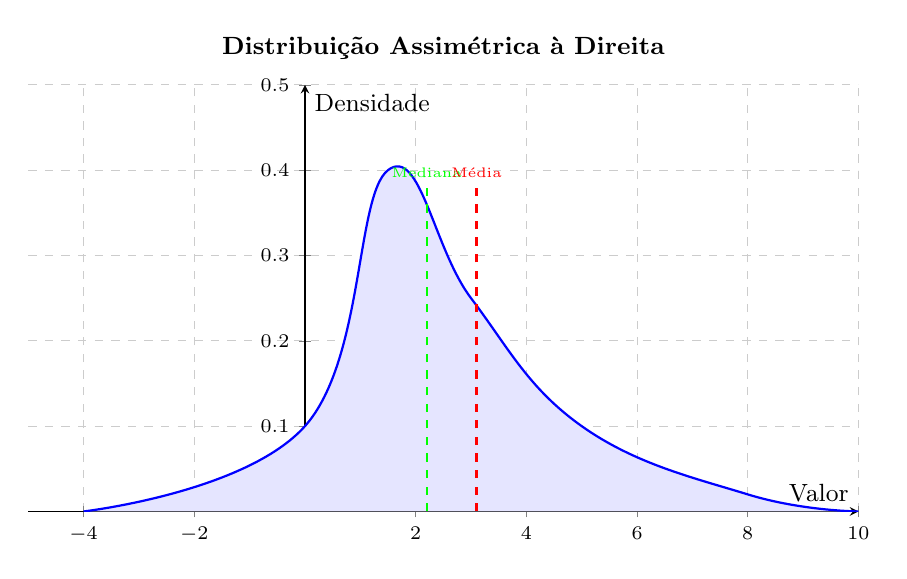
\begin{tikzpicture}
            \begin{axis}[
                width=\linewidth,
                height=7cm,
                xlabel={Valor},
                ylabel={Densidade},
                axis lines=middle,
                grid=major,
                grid style={dashed, gray!40},
                xmin=-5, xmax=10,
                ymin=0, ymax=0.5,
                legend pos=north west,
                title style={font=\bfseries\small},
                label style={font=\small},
                tick label style={font=\scriptsize},
                title={Distribuição Assimétrica à Direita}
            ]
                
                % Curva "desenhada" com smooth
                \addplot[
                    blue, thick, fill=blue!10,
                    smooth, tension=0.7 % 'tension' controla a suavidade
                ] coordinates {
                    (-4, 0)
                    (0, 0.1)
                    (1.5, 0.4)  % Pico (Moda)
                    (3, 0.25)
                    (5, 0.1)
                    (8, 0.02)
                    (10, 0)
                };

                % Mediana (mais perto do pico)
                \pgfmathsetmacro{\medianpos}{2.2} 
                \addplot[dashed, color=green, thick] coordinates {(\medianpos,0) (\medianpos,0.38)};
                \node[above, font=\tiny, green] at (axis cs:\medianpos,0.38) {Mediana};

                % Média (puxada pela cauda)
                \pgfmathsetmacro{\meanpos}{3.1} 
                \addplot[dashed, color=red, thick] coordinates {(\meanpos,0) (\meanpos,0.38)};
                \node[above, font=\tiny, red] at (axis cs:\meanpos,0.38) {Média};

            \end{axis}
        \end{tikzpicture}
        \caption{Assimétrica à direita (skew positivo).}%
        \label{fig:dist-skew-direita}
    \end{subfigure}
    \hfill 
    \begin{subfigure}[b]{0.48\textwidth}
        \centering
        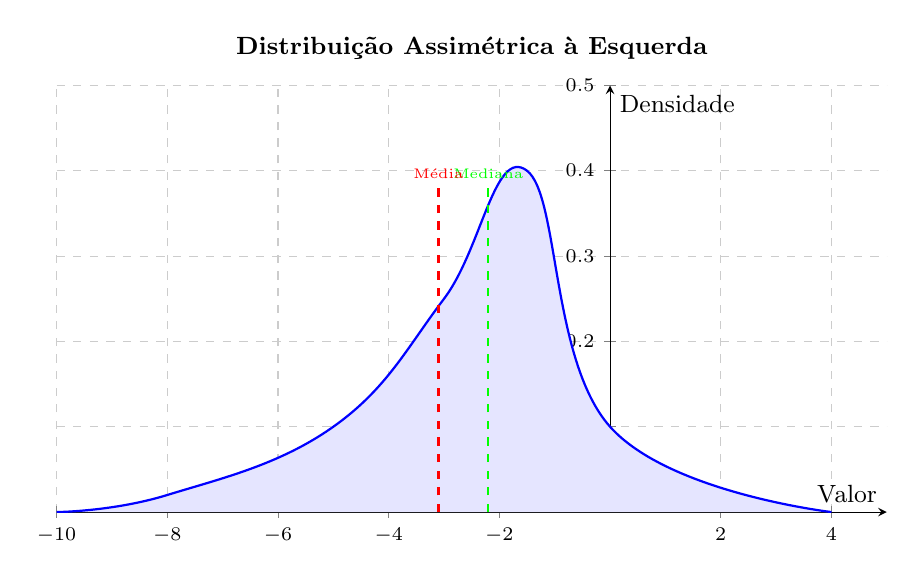
\begin{tikzpicture}
            \begin{axis}[
                width=\linewidth,
                height=7cm,
                xlabel={Valor},
                ylabel={Densidade},
                axis lines=middle,
                grid=major,
                grid style={dashed, gray!40},
                xmin=-10, xmax=5,
                ymin=0, ymax=0.5,
                legend pos=north east,
                title style={font=\bfseries\small},
                label style={font=\small},
                tick label style={font=\scriptsize},
                title={Distribuição Assimétrica à Esquerda}
            ]
                
                % Curva "desenhada" com smooth
                \addplot[
                    blue, thick, fill=blue!10,
                    smooth, tension=0.7
                ] coordinates {
                    (-10, 0)
                    (-8, 0.02)
                    (-5, 0.1)
                    (-3, 0.25)
                    (-1.5, 0.4) % Pico (Moda)
                    (0, 0.1)
                    (4, 0)
                };

                % Mediana (mais perto do pico)
                \pgfmathsetmacro{\medianneg}{-2.2} 
                \addplot[dashed, color=green, thick] coordinates {(\medianneg,0) (\medianneg,0.38)};
                \node[above, font=\tiny, green] at (axis cs:\medianneg,0.38) {Mediana};

                % Média (puxada pela cauda)
                \pgfmathsetmacro{\meannneg}{-3.1} 
                \addplot[dashed, color=red, thick] coordinates {(\meannneg,0) (\meannneg,0.38)};
                \node[above, font=\tiny, red] at (axis cs:\meannneg,0.38) {Média};

            \end{axis}
        \end{tikzpicture}
        \caption{Assimétrica à esquerda (skew negativo).}%
        \label{fig:dist-skew-esquerda}
    \end{subfigure}

    \caption{Exemplos de distribuições assimétricas (desenhadas) onde a média (vermelho) e a mediana (verde) divergem, justificando o uso da Perda Quantílica.}%
    \label{fig:distribuicoes-assimetricas}
    \fonte{O autor (2025).}
\end{figure}

Existe uma função de perda que consegue lidar justamente com esse cenário, em que os dados seguem uma distribuição assimétrica, ela é a perda quantílica, que foca em estudar como a perda acontece em diferentes quantis da distribuição. Ao utilizá-la é possível definir o quantil que será analisado, sendo possível escolher se ela irá funcionar de forma assimétrica, ou de forma parecida com o \textit{MAE}.

Além disso, existe uma outra função de perda que também não trabalha com o cálculo da média dos erros, ela é a $\epsilon$-insensível, sendo uma função essencial para a tarefas de regressão para máquinas de vetores de suporte. Neste caso, ao utilizar essa função, é possível definir uma ``margem de tolerância'' em que caso o erro esteja dentro dessa média, a perda não irá penalizar o modelo.

Dessa forma, é possível começar a seção explicando primeiro a perda quantílica.

\subsection{Perda Quantílica (Quantile Loss)}%
\index{Funções de Perda!Perda Quantílica (\textit{Quantile Loss})}

Antes de entender a perda quantílica de fato, será visto o conceito em que ela surgiu. No artigo \textit{Regression Quantiles} dos autores \textcite{regression-quantiles} estava sendo analisada uma nova técnica de regressão que se baseava nos quantis de uma distribuição. Como motivação para esse estudo, os autores discutem a ideia de que ``todos acreditam a lei de Gauss para os erros, porque eles acreditam que é um teorema matemático, e os matemáticos acreditam porque é um fato experimental'' \parencite{regression-quantiles}. Contudo, isso não é uma verdade absoluta, existem casos, como os vistos na introdução dessa seção que fogem da distribuição normal, e só técnicas mais conhecidas, como o \textit{MSE} para o cálculo dos erros com base na média, não são ideais para minimizar o erro de um modelo.

Tendo isso em mente, os pesquisadores discutem uma forma de minimizar a soma de perdas assimétricas, eles então definem a Equação~\ref{eq:soma-das-perdas-assimetricas}\footnote{Caso você leitor decida ler o artigo original dos pesquisadores, você verá um conjunto diferente de notações utilizadas, isso acontece pois neste livro elas foram adaptadas para condizer com as notações que já estavam sendo utilizadas anteriormente nos outros capítulos}.

\begin{equation}
    \Loss(w; \tau, y, X) = \sum_{j \text{ t.q. } y_j > \hat{y}_j} \tau |y_j -\hat{y}_j| + \sum_{j \text{ t.q. } y_j < \hat{y}_j} (1 -\tau) |y_j -\hat{y}_j|
    \label{eq:soma-das-perdas-assimetricas}
\end{equation}

Em que:

\begin{itemize}
    \item $\tau$ representa o quantil;
    \item $w$ representa os parâmetros do modelo, neste caso os pesos;
    \item $\hat{y}_j$ representa a predição do modelo;
\end{itemize}

A partir dessa expressão é possível analisar os casos, considerando a assimetria da perda

\textbf{Caso 1: O Valor real é maior que a previsão $(y_j > \hat{y}_j)$}

\begin{itemize}
    \item \textbf{Condição:} $y_j > \hat{y}_j$, indicando que o resíduo $u = (y_j - \hat{y}_j)$ é positivo.
    \item \textbf{Equação base:} A Equação~\ref{eq:soma-das-perdas-assimetricas} nos mostra que nesse caso é aplicado o termo $\tau|y_j - \hat{y}_j|$
    \item \textbf{Dedução:}
          \begin{enumerate}
        \item Como o resíduo $(y_j - \hat{y}_j)$ já é positivo, o valor absoluto de $|y_j - \hat{y}_j|$ é dado pela expressão $(y_j - \hat{y}_j)$;
        \item A perda se torna: $\tau (y_j - \hat{y}_j)$
    \end{enumerate}
\end{itemize}

\textbf{Caso 2: O valor real é menor que a previsão $(y_j < \hat{y}_j)$}

\begin{itemize}
    \item \textbf{Condição:} $y_j < \hat{y}_j$, o que significa que o resíduo $u = (y_j - \hat{y}_j)$ é negativo.
    \item \textbf{Equação base:} Voltando para a Equação~\ref{eq:soma-das-perdas-assimetricas}, ela nos mostra que nesse caso é aplicado o termo $(1 - \tau)|y_j - \hat{y}_j|$
    \item \textbf{Dedução:}
          \begin{enumerate}
        \item Como o resíduo $(y_j - \hat{y}_j)$ é negativo, o valor absoluto de $|y_j - \hat{y}_j|$ é dado por $-(y_j - \hat{y}_j)$, que também pode ser reescrito como $(\hat{y}_j - y_j)$;
        \item A perda se torna: $(1 - \tau)(\hat{y}_j - y_j)$
    \end{enumerate}
\end{itemize}

A partir desses dois casos, é possível criar a definição por partes da perda quantílica, também conhecida como \textit{quantile loss}. A expressão dessa função é dada pela Equação~\ref{eq:quantile-loss}. Neste caso, está sendo considerado que a situação $\hat{y} = y$ faz parte do primeiro caso estudado.

\begin{equacaodestaque}{Perda Quantílica (\textit{Quantile Loss})}
    \Loss_{\tau} (y_j, \hat{y}_j) = 
    \begin{cases} 
        \tau(y_j -\hat{y}_j) & \text{se } y_j \ge \hat{y}_j\\
        (1 -\tau) (\hat{y}_j -y_j) & \text{se } y_j < \hat{y}_j\end{cases}%
    \label{eq:quantile-loss}
\end{equacaodestaque}

Em que:

\begin{itemize}
    \item $y_j$ representa o valor real da j-ésima amostra;
    \item $\hat{y}_j$ representa o valor predito pelo modelo;
    \item $\tau$ representa o quantil.
\end{itemize}

Além dessa expressão, existe também uma versão compacta utilizando a função $\max$ para definir a função por partes da \textit{quantile loss} em apenas uma linha. Essa versão pode ser vista na Equação~\ref{eq:quantile-loss-com-max}.

\begin{equacaodestaque}{Perda Quantílica (\textit{Quantile Loss}) Reescrita Com a Função $\max$}
    \Loss_{\tau} (u)= \max(\tau u, (\tau-1 )u)%
    \label{eq:quantile-loss-com-max}
\end{equacaodestaque}

Considerando que $u = y - \hat{y}$, ou seja, o cálculo do resíduo.

Além das equação da perda quantílica, é possível também fazer a plotagem dos seus gráficos. Para isso, a Figura~\ref{fig:quantile-loss-tau05} mostra a representação em duas dimensões dessa função, enquanto a Figura~\ref{fig:quantile-loss-tau05} mostra a superfície da perda quantílica. Ambas mostram um cenário em que o valor de tau é dado por 0.5.

% --- FIGURA 1: FOCO NO TAU = 0.5 (MAE) ---
\begin{figure}[h!]
    \centering % Centraliza a figura na página

    % --- SUBFIGURA (a): Gráfico 2D da Perda Quantílica (Tau=0.5) ---
    \begin{subfigure}[b]{0.48\textwidth}
        \centering
        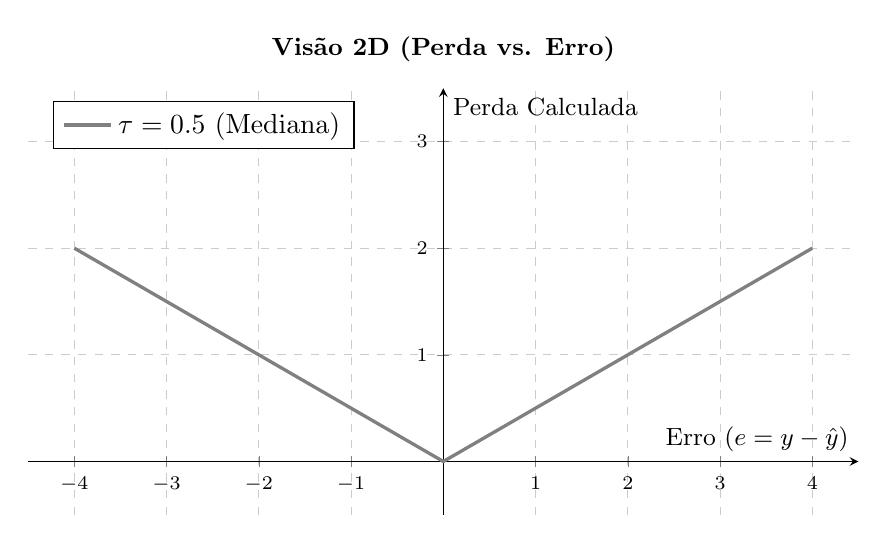
\begin{tikzpicture}
            \begin{axis}[
                width=\linewidth,  
                height=7cm,
                xlabel={Erro ($e = y - \hat{y}$)},
                ylabel={Perda Calculada},
                axis lines=middle,
                grid=major,
                grid style={dashed, gray!40},
                xmin=-4.5, xmax=4.5,
                ymin=-0.5, ymax=3.5,
                legend pos=north west,
                title style={font=\bfseries\small},
                label style={font=\small},
                tick label style={font=\scriptsize},
                title={Visão 2D (Perda vs. Erro)}
            ]
                % Tau = 0.5 (MAE)
                \addplot[domain=-4:4, samples=5, color=gray, very thick] {0.5*abs(x)};
                \addlegendentry{$\tau=0.5$ (Mediana)}
            \end{axis}
        \end{tikzpicture}
        \caption{Perda 2D para $\tau=0.5$.}%
        \label{fig:quantile-2d-tau05}
    \end{subfigure}
    \hfill 
    \begin{subfigure}[b]{0.48\textwidth}
        \centering
        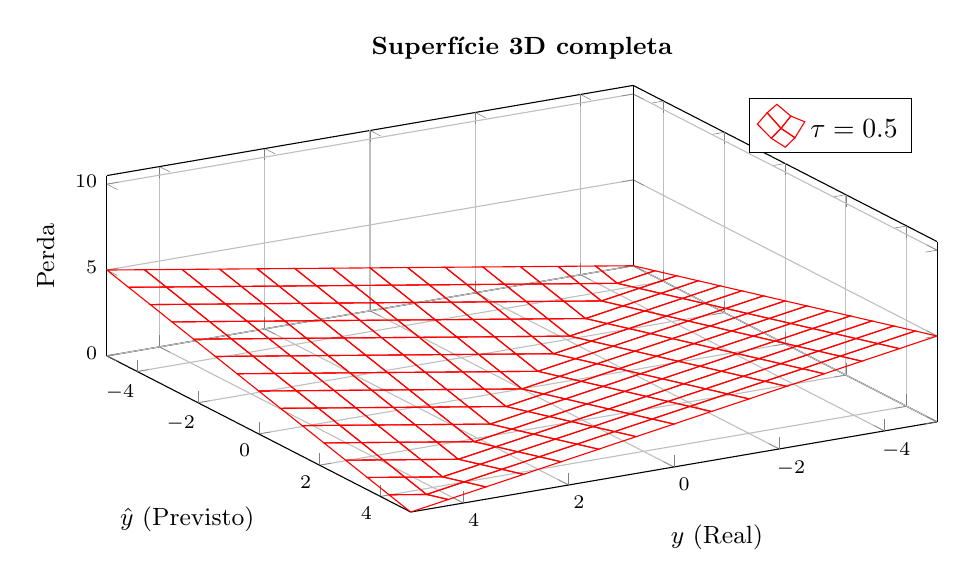
\begin{tikzpicture}
            \begin{axis}[
                width=\linewidth,
                height=7cm,
                xlabel={$y$ (Real)},
                ylabel={$\hat{y}$ (Previsto)},
                zlabel={Perda},
                grid=major,
                view={150}{45},
                zmin=0, zmax=10.5,
                legend pos=north east,
                title style={font=\bfseries\small},
                label style={font=\small},
                tick label style={font=\scriptsize},
                title={Superfície 3D completa}
            ]
                % Tau = 0.5 (Plano de fundo como superfície)
                \addplot3[
                    mesh,           
                    color=red,
                    domain=-5:5,
                    domain y=-5:5,
                    samples=15
                ] { 0.5*abs(x - y) };
                \addlegendentry{$\tau=0.5$}
            \end{axis}
        \end{tikzpicture}
        \caption{Superfície 3D para $\tau=0.5$.}%
        \label{fig:quantile-3d-tau05}
    \end{subfigure}

    \caption{Visualizações da Perda Quantílica para $\tau=0.5$ (Erro Absoluto Médio).}%
    \label{fig:quantile-loss-tau05}
    \fonte{O autor (2025).}
\end{figure}

Note que nessas figuras, a função é idêntica ao erro absoluto médio, o gráfico tem o formato em ``V'' característico dessa função. Isso acontece porque ao considerar calcular a perda quantílica para o quantil 50\% (indicado por 0.5), está sendo calculado a média dos dados, algo que também é feito utilizando outra expressão, ao utilizar o \textit{MAE} como função de perda.

Mas esse não é o cenário ideal para se utilizar a perda quantílica. Essa função realmente brilha quando precisa ser utilizada em cenários em que a distribuição de dados é irregular, e não segue a distribuição normal. Essa função tem uma propriedade única que pode se ajustar para penalizar de forma assimétrica os erros que um modelo comete. 

A Figura~\ref{fig:quantile-loss-grid} mostra esses diferentes cenários. Na Figura~\ref{fig:quantile-2d-tau09} e na Figura~\ref{fig:quantile-3d-tau09} é apresentado um caso em que $\tau = 0.9$, um cenário em que a perda quantílica irá penalizar fortemente as subestimações feitas pelo modelo. Isso acontece porque está sendo analisado o 90º percentil, o que significa que queremos uma previsão $\hat{y}$ que seja maior que 90\% dos valores reais $y$. Se o modelo subestima, ou seja $y > \hat{y}$, ele está falhando o seu objetivo, e terá um erro bem maior.

Já na Figura~\ref{fig:quantile-2d-tau01} e na Figura~\ref{fig:quantile-3d-tau01} está sendo apresentado o cenário contrário, é o quantil 10º que é analisado. Isso significa que queremos uma previsão que esteja abaixo dos 10\% dos valore reais, uma situação ideal para treinar o modelo a não superestimar os valores. Dado que ele será fortemente penalizado se ele fizer uma predição em que $y < \hat{y}$.

% --- FIGURA 2: GRADE 2x2 PARA TAU = 0.9 e TAU = 0.1 ---
\begin{figure}[h!]
    \centering

    % --- LINHA DE CIMA: TAU = 0.9 ---
    
    % Top-Esquerda: 2D para Tau = 0.9
    \begin{subfigure}[b]{0.48\textwidth}
        \centering
        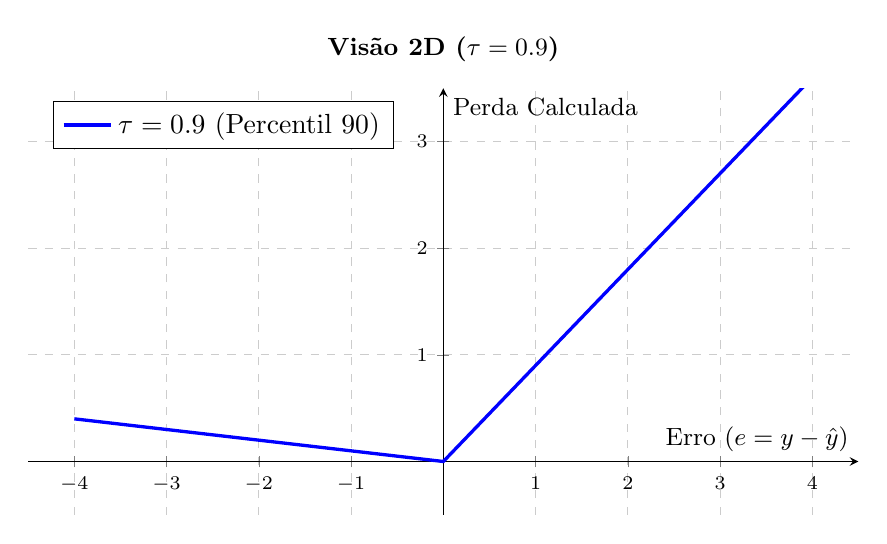
\begin{tikzpicture}
            \begin{axis}[
                width=\linewidth,  
                height=7cm,
                xlabel={Erro ($e = y - \hat{y}$)},
                ylabel={Perda Calculada},
                axis lines=middle,
                grid=major,
                grid style={dashed, gray!40},
                xmin=-4.5, xmax=4.5,
                ymin=-0.5, ymax=3.5,
                legend pos=north west,
                title style={font=\bfseries\small},
                label style={font=\small},
                tick label style={font=\scriptsize},
                title={Visão 2D ($\tau=0.9$)}
            ]
                % Tau = 0.9
                \addplot[domain=-4:4, samples=5, color=blue, very thick] {(x >= 0) ? (0.9*x) : ((1-0.9)*(-x))};
                \addlegendentry{$\tau=0.9$ (Percentil 90)}
            \end{axis}
        \end{tikzpicture}
        \caption{Perda 2D para $\tau=0.9$.}%
        \label{fig:quantile-2d-tau09}
    \end{subfigure}
    \hfill
    \begin{subfigure}[b]{0.48\textwidth}
        \centering
        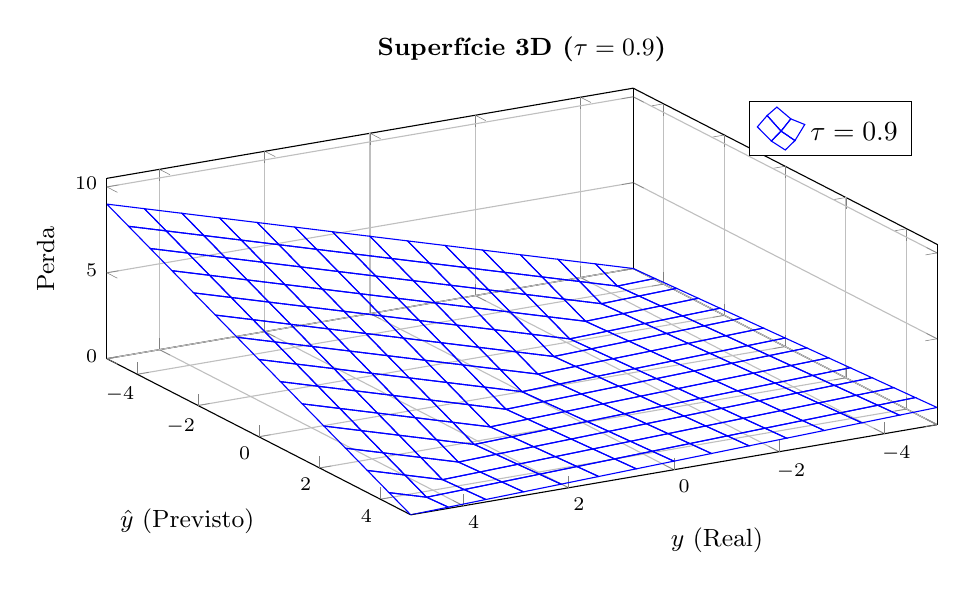
\begin{tikzpicture}
            \begin{axis}[
                width=\linewidth,
                height=7cm,
                xlabel={$y$ (Real)},
                ylabel={$\hat{y}$ (Previsto)},
                zlabel={Perda},
                grid=major,
                view={150}{45},
                zmin=0, zmax=10.5,
                legend pos=north east,
                title style={font=\bfseries\small},
                label style={font=\small},
                tick label style={font=\scriptsize},
                title={Superfície 3D ($\tau=0.9$)}
            ]
                % Tau = 0.9 (Malha)
                \addplot3[
                    mesh,           
                    color=blue,
                    domain=-5:5,
                    domain y=-5:5,
                    samples=15
                ] { (x - y >= 0) ? (0.9*(x - y)) : ((1-0.9)*(-(x - y))) };
                \addlegendentry{$\tau=0.9$}
            \end{axis}
        \end{tikzpicture}
        \caption{Superfície 3D para $\tau=0.9$.}%
        \label{fig:quantile-3d-tau09}
    \end{subfigure}

    \vspace{0.5cm} 

    \begin{subfigure}[b]{0.48\textwidth}
        \centering
        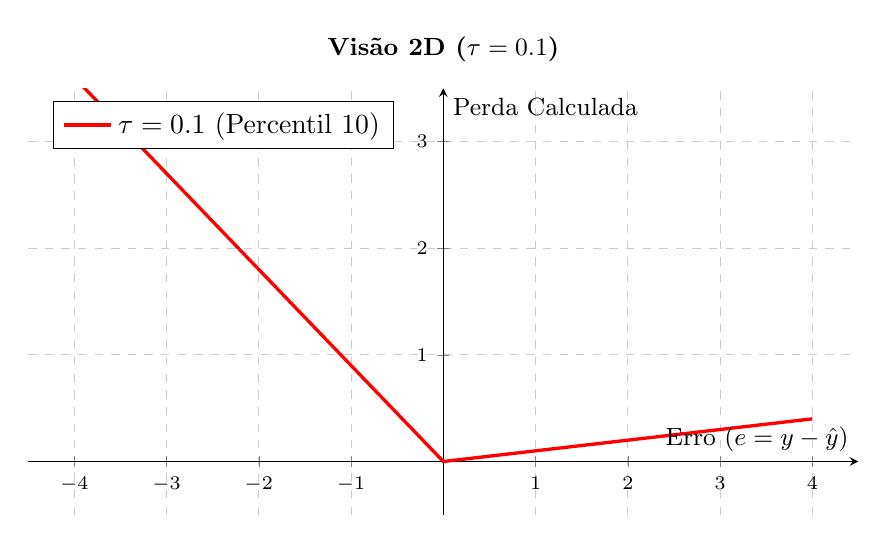
\begin{tikzpicture}
            \begin{axis}[
                width=\linewidth,  
                height=7cm,
                xlabel={Erro ($e = y - \hat{y}$)},
                ylabel={Perda Calculada},
                axis lines=middle,
                grid=major,
                grid style={dashed, gray!40},
                xmin=-4.5, xmax=4.5,
                ymin=-0.5, ymax=3.5,
                legend pos=north west,
                title style={font=\bfseries\small},
                label style={font=\small},
                tick label style={font=\scriptsize},
                title={Visão 2D ($\tau=0.1$)}
            ]
                % Tau = 0.1
                \addplot[domain=-4:4, samples=5, color=red, very thick] {(x >= 0) ? (0.1*x) : ((1-0.1)*(-x))};
                \addlegendentry{$\tau=0.1$ (Percentil 10)}
            \end{axis}
        \end{tikzpicture}
        \caption{Perda 2D para $\tau=0.1$.}%
        \label{fig:quantile-2d-tau01}
    \end{subfigure}
    \hfill
    \begin{subfigure}[b]{0.48\textwidth}
        \centering
        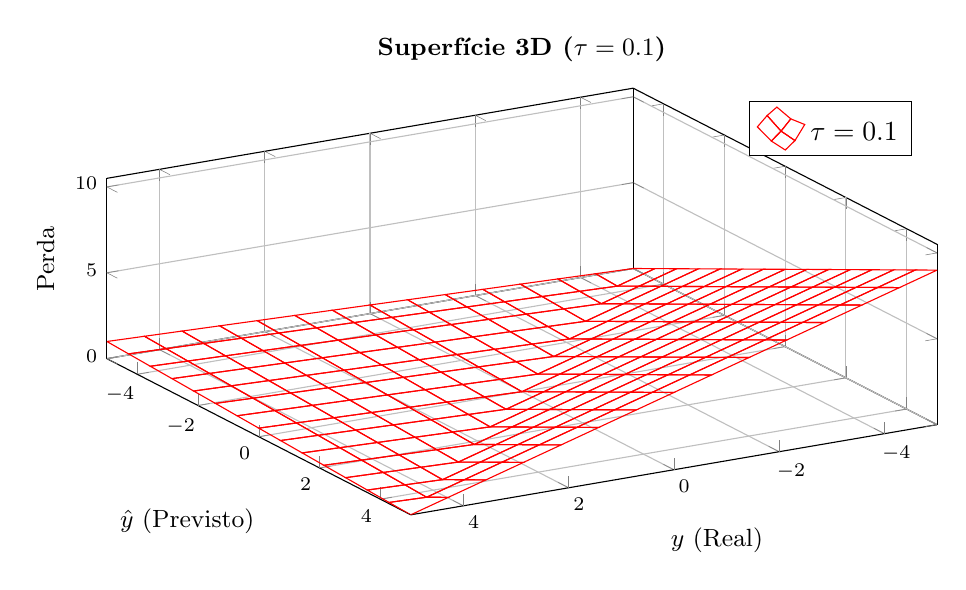
\begin{tikzpicture}
            \begin{axis}[
                width=\linewidth,
                height=7cm,
                xlabel={$y$ (Real)},
                ylabel={$\hat{y}$ (Previsto)},
                zlabel={Perda},
                grid=major,
                view={150}{45},
                zmin=0, zmax=10.5,
                legend pos=north east,
                title style={font=\bfseries\small},
                label style={font=\small},
                tick label style={font=\scriptsize},
                title={Superfície 3D ($\tau=0.1$)}
            ]
                % Tau = 0.1 (Malha)
                \addplot3[
                    mesh,           
                    color=red,
                    domain=-5:5,
                    domain y=-5:5,
                    samples=15
                ] { (x - y >= 0) ? (0.1*(x - y)) : ((1-0.1)*(-(x - y))) };
                \addlegendentry{$\tau=0.1$}
            \end{axis}
        \end{tikzpicture}
        \caption{Superfície 3D para $\tau=0.1$.}%
        \label{fig:quantile-3d-tau01}
    \end{subfigure}

    \caption{Visualizações das Perdas Quantílicas para os percentis 90 ($\tau=0.9$) e 10 ($\tau=0.1$).}%
    \label{fig:quantile-loss-grid}
    \fonte{O autor (2025).}
\end{figure}

\medskip
\begin{center}
 * * *
\end{center}
\medskip

\textbf{Características da Perda Quantílica} 
\vspace{1em}

\begin{itemize}
    \item \textbf{Convexa:} A perda quantílica é uma função convexa, dado que ela é o máximo de duas funções lineares (as quais são convexas). Isso significa que ela é uma função interessante para ser utilizada na otimização de redes neurais e outros modelos mais simples, pois será uma tarefa fácil encontrar um ponto de mínimo. Contudo, voltando para o cenário de redes neurais, isso não é necessariamente garantido, visto que devido a quantidade de camadas densas e de funções de ativação não-lineares pode fazer com que a perda quantílica se torne não convexa;
    \item \textbf{Penalização assimétrica:} Como foi visto anteriormente, a \textit{quantile loss} é uma função assimétrica, exceto no caso em que $\tau = 0.5$, e como o parâmetro $\tau$ é definido ao treinar ao modelo, cabe a quem estiver treinado o modelo definir se ele quer que a função penalize mais as subestimações ou as superestimações, a depender do problema que está sendo considerado;
    \item \textbf{Não diferenciabilidade no resíduo 0:} \textcite{LossesArticle} apontam que no cenário em que $\hat{y}_j = y_j$, semelhante ao \textit{MAE} essa função não é diferenciável, sendo necessárias técnicas como o cálculo do subgradiente para permitir a otimização nesse ponto. Essa não diferenciabilidade acontece pois neste ponto a função apresenta uma ``quina'', algo que afeta o cálculo das derivadas parciais, e consequentemente do vetor gradiente, nesse ponto.
\end{itemize}

\medskip
\begin{center}
 * * *
\end{center}
\medskip

Vista o surgimento da perda quantílica, a sua definição matemática, os seus gráficos e algumas de suas propriedades, é possível agora discutir a sua derivada. Para isso, deve-se derivar as duas expressões da Equação~\ref{eq:quantile-loss} e escrever o seu resultado em uma função por partes. Neste caso está sendo considerado que não existe um valor para o cenário em que a predição é igual ao valor real, ou seja, $\hat{y}_j = y_j$, dado que este é um ponto de descontinuidade dessa função.

Dessa forma, a derivada parcial da perda quantílica em relação a predição feita pelo modelo é dada pela Equação~\ref{eq:quantile-loss-derivada}. Além disso, você pode ver na equação que está sendo indicado os cenários de superestimação e subestimação, de forma a simplificar como os erros do modelo serão corrigidos ao retropropagar o gradiente para as camadas.

\begin{equacaodestaque}{Derivada Parcial da Perda Quantílica em Relação a Predição $\hat{y}_j$}
    \frac{\partial\Loss_{\tau}}{\partial\hat{y}_j} = 
    \begin{cases} 
        -(1 - \tau) & \text{se } y_j < \hat{y}_j \text{ (superestimação)}\\
        -\tau & \text{se } y_j > \hat{y}_j \text{ (subestimação)}
    \end{cases}%
    \label{eq:quantile-loss-derivada}
\end{equacaodestaque}

Além disso, cabe também ser a sua derivada, a qual está presente na Figura~\ref{fig:quantile-loss-derivada}, neste caso está sendo apresentado somente a sua visualização em duas dimensões. Perceba que o gráfico em que $\tau = 0.5$ é igual o gráfico da derivada do erro absoluto médio.

\begin{figure}[h!]
    \centering
    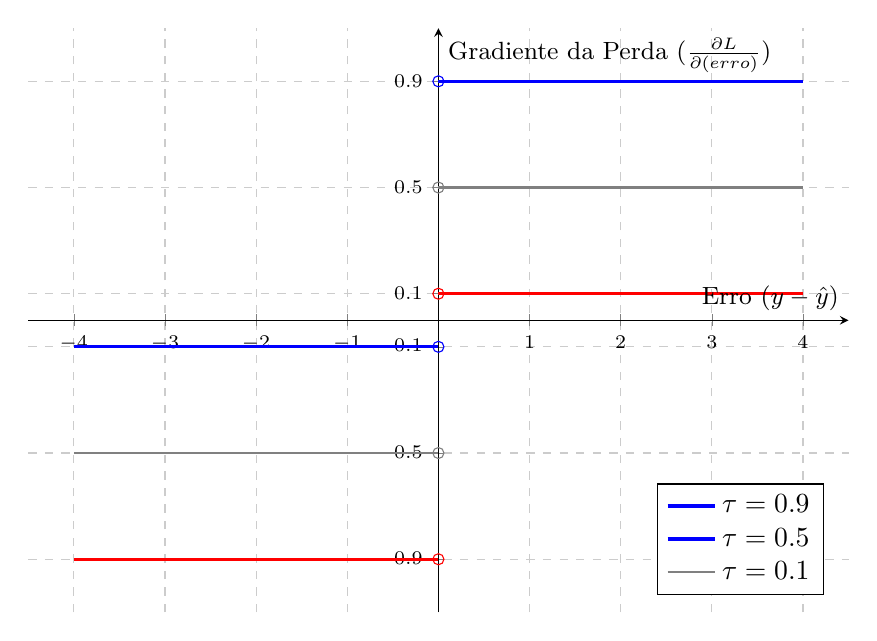
\begin{tikzpicture}
        \begin{axis}[
            xlabel={Erro ($y - \hat{y}$)},
            ylabel={Gradiente da Perda ($\frac{\partial L}{\partial (\text{erro})}$)},
            axis lines=middle,
            grid=major,
            grid style={dashed, gray!40},
            xmin=-4.5, xmax=4.5,
            ymin=-1.1, ymax=1.1,
            ytick={-0.9, -0.5, -0.1, 0, 0.1, 0.5, 0.9},
            legend pos=south east,
            width=12cm,
            height=9cm,
            title style={font=\bfseries},
            label style={font=\small},
            tick label style={font=\scriptsize}
        ]
            % Linhas para Tau = 0.9
            \addplot[const plot, color=blue, very thick] coordinates {(-4, 0.9-1) (0, 0.9-1)};
            \addplot[const plot, color=blue, very thick] coordinates {(0, 0.9) (4, 0.9)};
            \addlegendentry{$\tau=0.9$}
            
            % Linhas para Tau = 0.5
            \addplot[const plot, color=gray, thick] coordinates {(-4, 0.5-1) (0, 0.5-1)};
            \addplot[const plot, color=gray, thick] coordinates {(0, 0.5) (4, 0.5)};
            \addlegendentry{$\tau=0.5$}

            % Linhas para Tau = 0.1
            \addplot[const plot, color=red, very thick] coordinates {(-4, 0.1-1) (0, 0.1-1)};
            \addplot[const plot, color=red, very thick] coordinates {(0, 0.1) (4, 0.1)};
            \addlegendentry{$\tau=0.1$}

            % Círculos abertos para a descontinuidade
            \addplot[only marks, mark=o, color=blue, mark size=2pt] coordinates {(0, -0.1) (0, 0.9)};
            \addplot[only marks, mark=o, color=gray, mark size=2pt] coordinates {(0, -0.5) (0, 0.5)};
            \addplot[only marks, mark=o, color=red, mark size=2pt] coordinates {(0, -0.9) (0, 0.1)};
        \end{axis}
    \end{tikzpicture}
    \caption{Gráfico da derivada da Perda Quantílica (em relação ao erro).}%
    \label{fig:quantile-loss-derivada}
    \fonte{O autor (2025).}
\end{figure}

\medskip
\begin{center}
 * * *
\end{center}
\medskip

\textbf{Algumas Aplicações da Perda Quantílica em Problemas de Regressão}%
\index{Aplicações práticas! Perda quantílica}
\vspace{1em}

Agora que já é conhecida a perda quantílica, é possível discutir alguns cenários em que essa função é utilizada para servir de guia para a otimização de modelos. Uma situação que ela está muito presente é na análise do valor em risco ou \textit{value at risk} (\textit{VaR}) em inglês. O \textit{VaR} é uma medida de risco que estima a perda potencial máxima que pode acontecer um determinado portfólio durante um período de tempo definido, isso é estimado dentro de um nível de confiança especificado. Por exemplo, caso queira ser descoberto o \textit{VaR} a 99\%, é preciso calcular o 1º quantil da distribuição de perdas e ganhos. Esse é um dos cenários que está presente em alguns dos trabalhos apresentados nessa seção, em que os autores optam pela perda quantílica para resolver esse problema.

Dito isso, vale citar os trabalhos: 

\begin{itemize}
    \item \textbf{Aplicação 1 (Área):} Em \textit{Mixed–frequency quantile regressions to forecast Value–at–Risk and Expected Shortfall}, \textcite{candila2023mixedfrequencyquantileregressionsforecast} utilizam da regressão quantílica como uma forma de prever o \textit{VaR} e o \textit{expected shortfall} (\textit{ES}), para isso, eles criam utilizam de uma técnica diferente, em que é feito o uso de regressões quantílicas de frequência mista. Para fazer isso, os autores combinam dados macroêconomicos de baixa frequência (que são mensais), com dados de mercado de alta frequência (os quais são diários) \parencite{candila2023mixedfrequencyquantileregressionsforecast}. Além disso, \textcite{candila2023mixedfrequencyquantileregressionsforecast} exploram esse novo modelo criado com dados reais, utilizando duas commodities energéticas chamadas Crude Oil and Gasoline futures;
    \item \textbf{Aplicação 2 (Área):} Outro trabalho que também faz uso da regressão quantílica é o \textit{CAViaR: Conditional Autoregressive Value at Risk by Regression Quantiles}, nele, \textcite{Engle2004CAViaR} apresenta o \textit{Conditional Autoregressive Value at Risk} ou \textit{CAViaR}. O \textit{CAViaR}, como os autores explicam no texto, propõe uma alternativa diferente para calcular o \textit{VaR}, ao invés de ser modelado toda a distribuição, com o \textit{CAViaR} é calculado apenas o quantil desejado, isso pode ser calculado com o uso da regressão quantílica, e consequentemente com a função de perda quantílica \parencite{Engle2004CAViaR};
    \item \textbf{Aplicação 3 (Área):} Além disso, vale citar também o artigo \textit{Reforming health care: Evidence from quantile regressions for counts} de \textcite{WINKELMANN2006131}, nele, a regressão quantílica para contagens é utilizada para estimar o efeito de uma reforma na saúde sobre a frequência de consultas médicas individuais. O autor justifica a escolha de ser feita uma regressão quantílica, e não uma técnica mais comum, como a dos mínimos quadrados, pois ele considera que esse é um problema em que os efeitos da reforma são diferentes em cada uma das partes da distribuição \parencite{WINKELMANN2006131}. Neste cenário, em que a distribuição de dados foge da distribuição normal, uma alternativa para lidar com isso é utilizar a perda quantílica\footnote{Além disso, caso você leitor esteja procurando funções de perdas para lidar com distribuições que não seguem a distribuição normal, vale a pena dar uma olhada na Seção~\ref{sec:perdas-baseadas-em-distribuicoes-de-dados}. Nela, são explicadas duas funções de perda que podem ser utilizadas nesse cenário: a perda de Poisson e a perda de Tweedie.}.
\end{itemize}

\medskip
\begin{center}
 * * *
\end{center}
\medskip

Além da perda quantílica, que é usada nos problemas de regressão quantílica, e que faz o cálculo dos erros considerando uma distribuição irregular dos dados, e por isso não faz o uso da média dos erros para encontrar a perda, existem outras funções que possuem essa mesma característica. Uma dessas funções é a epsilon-insensível, que é essencial para resolver os problemas de regressão para modelos de máquinas de vetores de suporte (\textit{SVMs}). Ela será explicada em seguida.

\subsection{Perda Epsilon-Insensível}%
\index{Funções de Perda!Perda Epsilon-Insensível}

Para explicar a perda $\epsilon$-insensível é preciso antes entender o cenário em que essa função surgiu, e como ela está relacionada com os modelos de regressão para as \textit{SVMs}. Um do artigos que explica a criação desse modelo de aprendizado de máquina para a tarefa de regressão é o \textit{Support Vector Regression Machines} dos pesquisadores \textcite{SupportVectorRegressionMachines}, nele, os autores detalham um novo uso das máquinas de vetores desenvolvidas por Vapnik, as quais antes eram utilizadas para resolver problemas de classificação.

\textcite{SupportVectorRegressionMachines} começam o artigo explicando um problema, eles possuem uma função $G(x)$ (chamada de verdade), sendo uma função que recebe um vetor $x$ (chamado de espaço de entradas), esse vetor $x$ possui $d$ componentes, sendo do tipo $x^t = [x_1, x_2, ..., x_d]$. Além disso, existe também uma família de funções $F(x, w)$ parametrizadas por $w$ \parencite{SupportVectorRegressionMachines}. O Objeto dos autores é encontrar um parâmetro $\hat{w}$ que é uma estimativa de $w$ a partir de observar um conjunto de $N$ instâncias de treinamento \parencite{SupportVectorRegressionMachines}.

Uma das aproximações para resolver esse problema é dada Equação xx como explicam \textcite{SupportVectorRegressionMachines}.

\begin{equation}
    F = (x, \hat{[w]}) = \sum_{i = 1}^N (\alpha_i^*- \alpha_i)(v_i^tx + 1)^p + b
    \label{eq:svms-para-regressao}
\end{equation}

Além disso, eles possuem também a função objetiva que querem minimizar, ela é dada pela Equação xx

\begin{equation}
    U \sum_{j = 1}^N L [y_j- F(v_j, \hat{w})] + ||\hat{w}||^2
\end{equation}

Note que essa função objetiva faz o uso de uma função de perda em sua fórmula, essa função é dada pela $\epsilon$-insensível, a qual pode ser vista na Equação~\ref{eq:epsilon-insensitive-loss}

\begin{equacaodestaque}{Perda Epsilon-Insensível (\textit{$\epsilon$-Insensitive Loss})}
    \Loss_{\epsilon}(y,\hat{y}) = 
    \begin{cases} 
        0 & \text{se } |y -\hat{y}| < \epsilon\\
        |y -\hat{y}| -\epsilon& \text{se } |y -\hat{y}| \ge\epsilon\end{cases}%
    \label{eq:epsilon-insensitive-loss}
\end{equacaodestaque}

Em que:

\begin{itemize}
    \item $y_j$ representa o valor real da j-ésima amostra;
    \item $\hat{y}_j$ representa o valor predito pelo modelo;
    \item $\epsilon$ ...
\end{itemize}

O objetivo de utilizar essa função de perda em máquinas de vetores de suporte para problemas de regressão é criar uma margem em que o erro do modelo não seja penalizado. O tamanho dessa margem é dado pelo termo $\epsilon$, além disso, fora desse intervalo o erro é penalizado de forma linear, assim como no erro absoluto médio. Isso pode ser visto de forma mais intuitiva nos gráficos da Figura~\ref{fig:epsilon-insensitive-loss}, no gráfico da esquerda (a Figura~\ref{fig:epsilon-2d}) é possível ver a representação em duas dimensões da perda, enquanto no gráfico da direta (a Figura~\ref{fig:epsilon-3d}) está representado a superfície dessa função no espaço.

\begin{figure}[h!]
    \centering 

    \begin{subfigure}[b]{0.48\textwidth}
        \centering
        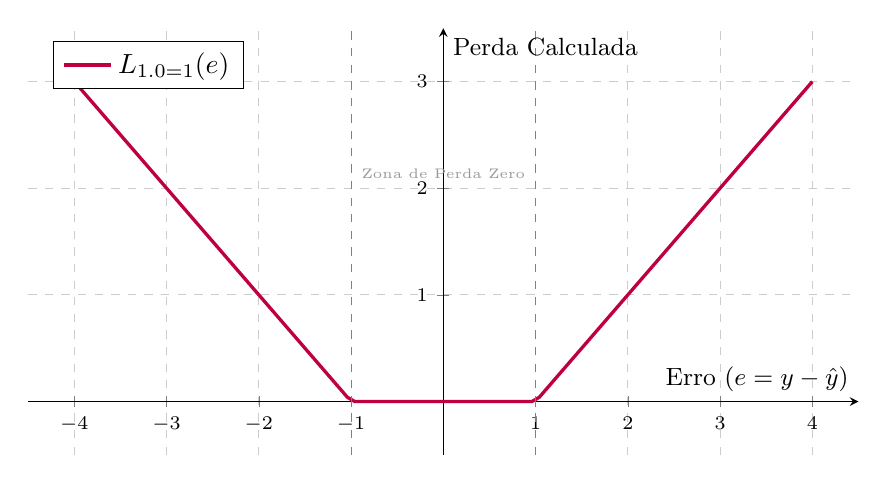
\begin{tikzpicture}
            % Define o valor de epsilon
            \def\epsilon{1.0}
            
            \begin{axis}[
                % Dimensões ajustadas para caber lado a lado
                width=\linewidth,  
                height=7cm,
                xlabel={Erro ($e = y - \hat{y}$)},
                ylabel={Perda Calculada},
                axis lines=middle,
                grid=major,
                grid style={dashed, gray!40},
                xmin=-4.5, xmax=4.5,        % Limites do seu gráfico
                ymin=-0.5, ymax=3.5,         % Limites do seu gráfico
                legend pos=north west,
                title style={font=\bfseries\small},
                label style={font=\small},
                tick label style={font=\scriptsize}
            ]
                % Gráfico da função
                \addplot[
                    domain=-4:4, 
                    samples=101,
                    color=purple, 
                    very thick
                ] {max(0, abs(x) - \epsilon)};
                
                \addlegendentry{$L_{\epsilon=1}(e)$}

                % Linhas tracejadas para marcar a margem epsilon
                \draw[dashed, gray] (axis cs:-\epsilon, -0.5) -- (axis cs:-\epsilon, 3.5);
                \draw[dashed, gray] (axis cs:\epsilon, -0.5) -- (axis cs:\epsilon, 3.5);
                \node[above, gray!80, font=\tiny] at (axis cs:0, 2) {Zona de Perda Zero};
            \end{axis}
        \end{tikzpicture}
        \caption{Visão 2D (Perda vs. Erro).}%
        \label{fig:epsilon-2d}
    \end{subfigure}
    \hfill
    \begin{subfigure}[b]{0.48\textwidth}
        \centering
        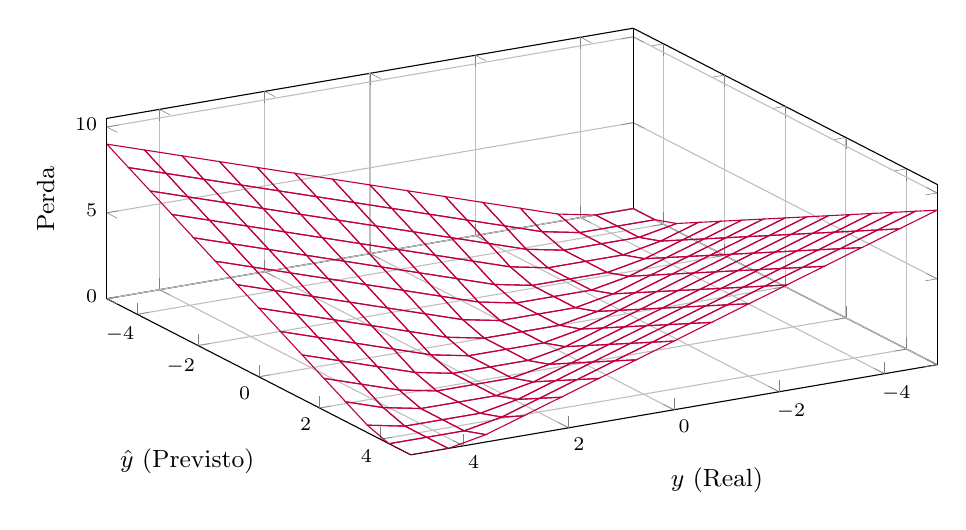
\begin{tikzpicture}
            % Define o valor de epsilon
            \def\epsilon{1.0}
            
            \begin{axis}[
                % Dimensões consistentes com o gráfico (a)
                width=\linewidth,
                height=7cm,
                xlabel={$y$ (Real)},
                ylabel={$\hat{y}$ (Previsto)},
                zlabel={Perda},
                grid=major,
                view={150}{45}, % Mesmo ângulo de visão do seu template
                zmin=0, zmax=10.5, % Ajustado para max(0, abs(10) - 1) = 9
                title style={font=\bfseries\small},
                label style={font=\small},
                tick label style={font=\scriptsize}
            ]
                % Gráfico da superfície da Epsilon-Insensitive Loss
                \addplot3[
                    mesh,           
                    color=purple,   % Cor consistente com o gráfico 2D
                    shader=interp,  
                    domain=-5:5,    % Mesmo domínio do seu template
                    domain y=-5:5,  % Mesmo domínio do seu template
                    samples=15      % Mesma resolução da malha
                ] { max(0, abs(x - y) - \epsilon) }; % A função Epsilon-Insensitive 3D
            \end{axis}
        \end{tikzpicture}
        \caption{Superfície 3D completa.}%
        \label{fig:epsilon-3d}
    \end{subfigure}

    \caption{Visualizações da função de perda Epsilon-Insensível (\textit{Epsilon-Insensitive Loss}, $\epsilon=1$) em duas e em três dimensões.}%
    \label{fig:epsilon-insensitive-loss}
    \fonte{O autor (2025).}
\end{figure}

\medskip
\begin{center}
 * * *
\end{center}
\medskip

\textbf{Características da Perda Epsilon-Insensível}
\vspace{1em}

\begin{itemize}
    \item \textbf{Robustez para \textit{outliers}:} Uma das características da perda $\epsilon$-insensível é a sua robustez para \textit{outliers}, isso acontece devido ao jeito que ela lida com esse tipo de dado. Diferente do erro quadrático médio, que penaliza fortemente as predições do modelo $\hat{y}$ que estão muito distantes do valor real $y$ e por isso, ao ser aplicada um conjunto que possui muitos \textit{outliers} o modelo que faz uso dessa perda não irá performar tão bem. Na perda $\epsilon$-insensível isso não acontece de forma tão drástica, uma vez que ela penaliza os erros de forma linear.
    \item \textbf{Não-diferenciabilidade em erro $=$ $\epsilon$:} Note no gráfico dessa função de perda que existem duas ``quinas'' nos pontos em que o erro é igual a $\epsilon$, isso não impede a função de ser contínua nesse ponto, mas não permite que ela seja diferenciada, algo que pode atrapalhar ao ser combinada com otimizadores que fazem uso do cálculo do gradiente.
    \item \textbf{Zona de perda zero:} Perceba pelo gráfico da perda $\epsilon$-insensível que diferente das outras perdas em que elas possuíam um único ponto de mínimo no qual a perda era zero, aqui isso não acontece, existe uma reta com tamanho definido por $\epsilon$ que mostra que a perda é zero, qualquer ponto que estiver dentro dessa reta estará no ponto de mínimo da função. Isso é propriedade interessante, pois significa que existem mais locais para pontos de mínimos, o que em teoria pode fazer com que a função seja mais fácil para ser otimizada.
\end{itemize}

\medskip
\begin{center}
 * * *
\end{center}
\medskip

Cabe agora discutir também o cálculo da derivada dessa função, que será útil para criação do vetor gradiente e da retropropagação dos erros. Para calculá-la é preciso derivar as duas expressões da Equação~\ref{eq:epsilon-insensitive-loss}, contudo, assim como no erro absoluto médio que foi preciso fazer o cálculo da derivada com auxílio de subgradientes por conta dos pontos de não-diferenciabilidade, aqui o processo é semelhante. Com isso, é possível chegar na expressão da Equação~\ref{eq:epsilon-insensitive-derivada} para a derivada parcial em relação a predição do modelo $\hat{y}$ para a perda $\epsilon$-insensível.

\begin{equacaodestaque}{Derivada da Perda Epsilon-Insensível}
    \frac{\partial\Loss_{\epsilon}}{\partial\hat{y}} = 
    \begin{cases} 
        -1 & \text{se } \hat{y} -y > \epsilon\\
        0 & \text{se } |\hat{y} -y| \le\epsilon\\
        1 & \text{se } \hat{y} -y < -\epsilon\end{cases}%
    \label{eq:epsilon-insensitive-derivada}
\end{equacaodestaque}

Tendo sua derivada calculada, o próximo passo é fazer a plotagem do seu gráfico, o qual pode ser visto na Figura~\ref{fig:epsilon-derivada-completa}. No gráfico da esquerda, na Figura~\ref{fig:epsilon-derivada-2d}, está a representação de uma vista em duas dimensões da perda $\epsilon$-insensível. Já no gráfico da direta, na Figura~\ref{fig:epsilon-derivada-3d}, está a superfície da derivada parcial da perda em relação as predições $\hat{y}$ do modelo.

\begin{figure}[h!]
    \centering % Centraliza a figura

    % --- Define o valor de epsilon e o ponto de corte (y real) ---
    \def\epsilon{1.0}
    \def\yreal{5.0} % Valor de y (Real) para o corte 2D

    % --- SUBFIGURA (a): Gráfico 2D da Derivada (Corte em y=5) ---
    \begin{subfigure}[b]{0.48\textwidth}
        \centering
        \begin{tikzpicture}
            \begin{axis}[
                width=\linewidth,  
                height=7cm,
                title={Visão 2D (corte em $y=\yreal$)},
                xlabel={Valor Previsto ($\hat{y}$)},
                ylabel={Gradiente ($\frac{\partial L}{\partial \hat{y}}$)},
                axis lines=middle,
                grid=major,
                grid style={dashed, gray!40},
                xmin=0, xmax=10,
                ymin=-1.5, ymax=1.5,
                ytick={-1, 0, 1},
                legend pos=north west,
                title style={font=\bfseries\small},
                label style={font=\small},
                tick label style={font=\scriptsize}
            ]
                
                % --- Gráfico da Derivada por partes (const plot) ---
                % Baseado na Equação 10.23: L' = 1 se y_hat < y - eps
                \addplot[const plot, color=blue, very thick, opacity=0.8] 
                    coordinates { (0, 1) (\yreal - \epsilon, 1) };
                \addlegendentry{$\hat{y} - y < -\epsilon \implies +1$}
                
                % L' = 0 se |y_hat - y| <= eps
                \addplot[const plot, color=gray, very thick, opacity=0.8] 
                    coordinates { (\yreal - \epsilon, 0) (\yreal + \epsilon, 0) };
                \addlegendentry{$|\hat{y} - y| \le \epsilon \implies 0$}
                
                % L' = -1 se y_hat - y > eps
                \addplot[const plot, color=red, very thick, opacity=0.8] 
                    coordinates { (\yreal + \epsilon, -1) (10, -1) };
                \addlegendentry{$\hat{y} - y > \epsilon \implies -1$}

                % --- Linhas de marcação ---
                % Linha vertical para o valor real
                \draw[dashed, gray] (axis cs:\yreal, -1.5) -- (axis cs:\yreal, 1.5);
                \node[above, gray!80, font=\tiny] at (axis cs:\yreal, 1.5) {Valor Real};
                
                % Linhas verticais para a margem epsilon
                \draw[dashed, black!60] (axis cs:\yreal-\epsilon, -1.5) -- (axis cs:\yreal-\epsilon, 1.5);
                \draw[dashed, black!60] (axis cs:\yreal+\epsilon, -1.5) -- (axis cs:\yreal+\epsilon, 1.5);

            \end{axis}
        \end{tikzpicture}
        \caption{Visão 2D (corte em $y=\yreal$).}%
        \label{fig:epsilon-derivada-2d}
    \end{subfigure}
    \hfill 
    \begin{subfigure}[b]{0.48\textwidth}
        \centering
        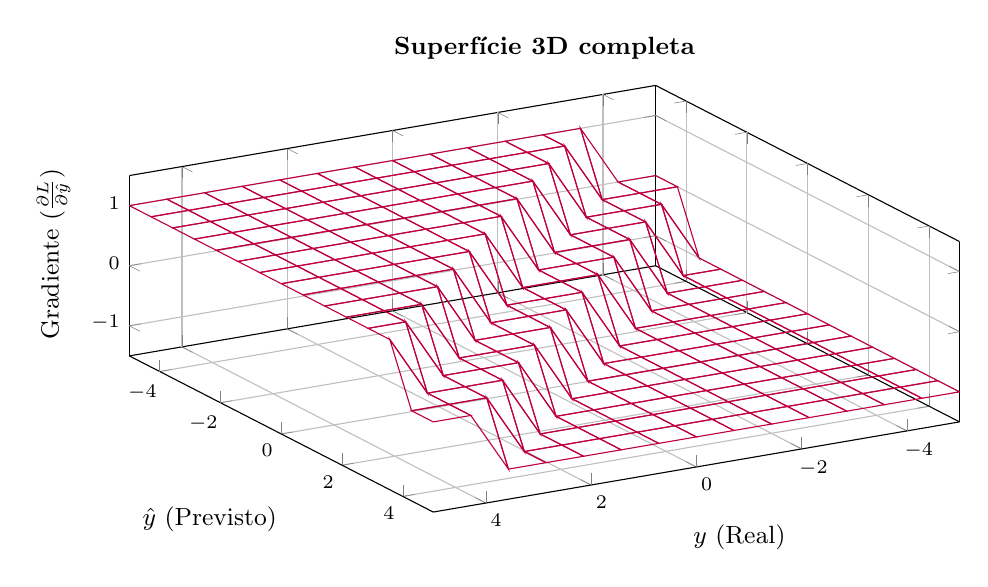
\begin{tikzpicture}
            \begin{axis}[
                width=\linewidth,
                height=7cm,
                title={Superfície 3D completa},
                xlabel={$y$ (Real)},
                ylabel={$\hat{y}$ (Previsto)},
                zlabel={Gradiente ($\frac{\partial L}{\partial \hat{y}}$)},
                grid=major,
                view={150}{45}, % Mesmo ângulo de visão do seu template
                zmin=-1.5, zmax=1.5,
                ztick={-1, 0, 1}, % Ticks exatos da derivada
                title style={font=\bfseries\small},
                label style={font=\small},
                tick label style={font=\scriptsize},
                colormap/viridis % Mapa de cores do seu template
            ]
                % Gráfico da superfície da Derivada da Epsilon-Insensitive Loss
                % x = y (Real), y = y_hat (Previsto)
                % Fórmula (Equação 10.23):
                % (y - x > epsilon) ? -1 : ( (y - x < -epsilon) ? 1 : 0 )
                \addplot3[
                    mesh,           
                    color=purple,   % Cor consistente com o gráfico 2D
                    shader=interp,  
                    domain=-5:5,    % Mesmo domínio do seu template
                    domain y=-5:5,  % Mesmo domínio do seu template
                    samples=15      % Mesma resolução da malha
                ] { (y - x > \epsilon) ? -1 : ( (y - x < -\epsilon) ? 1 : 0 ) }; 
            \end{axis}
        \end{tikzpicture}
        \caption{Superfície 3D completa.}%
        \label{fig:epsilon-derivada-3d}
    \end{subfigure}

    \caption{Visualizações da derivada (gradiente) da função de perda Epsilon-Insensível ($\epsilon=1$).}%
    \label{fig:epsilon-derivada-completa}
    \fonte{O autor (2025).}
\end{figure}

Perceba como as características da função refletem em sua derivada, nas retas definidas por $\epsilon$ em que a perda é zero, consequentemente a sua derivada também será zero, algo que pode ser visto no gráfico da Figura~\ref{fig:epsilon-derivada-2d}, existem uma lacuna onde a função também é zero. Além disso, note que nos pontos em que acontece o ``bico'' da função original, eles viram uma reta vertical na derivada, como a Figura~\ref{fig:epsilon-derivada-3d}. Isso é interessante pois nos mostra de forma mais direta, quais serão os pontos em que será difícil de calcular o gradiente e com isso ele irá nos causar problemas.

Essa análise de descontinuidade pode ser feita também com o próprio gráfico da função, mas como o cálculo da derivada depende que a função seja contínua no ponto desejado, ao plotar os gráficos de uma função de perda, é possível ter uma noção mais explícita dos pontos ``problema'' de uma função de perda.

\medskip
\begin{center}
 * * *
\end{center}
\medskip

\textbf{Algumas Aplicações da Perda Epsilon-Insensível em Problemas de Regressão}%
\index{Aplicações práticas! Perda epsilon-insensível}
\vspace{1em}

\begin{itemize}
    \item \textbf{Aplicação 1 (Área):}
    \item \textbf{Aplicação 2 (Área):}
    \item \textbf{Aplicação 3 (Área):}
    \item \textbf{Aplicação 4 (Área):}
\end{itemize}

\section{Perdas Baseadas em Distribuições de Dados}%
\label{sec:perdas-baseadas-em-distribuicoes-de-dados}

Exceto pela perda $\epsilon$-insensível que trabalhava com distribuições que não eram simétricas, a maioria das perdas trabalhadas até agora neste capítulo possuem uma característica em comum: são perdas utilizadas para dados que seguem a distribuição normal. Foi possível ver isso inclusive na explicação sobre o erro quadrático médio, e como Gauss prova que o método dos mínimos quadrados é uma solução ideal para ser utilizado em cenários em que os dados seguem a distribuição Gaussiana.

Contudo, mesmo a distribuição normal sendo a mais comum para modelar os diferentes problemas que envolvem regressão, existem também outras distribuições que são igualmente importante. Essa seção foca em explicar três funções de perda que são utilizadas para trabalhar com distribuições específicas, são elas: a perda de Poisson, a perda Gamma e a perda de Tweedie.

Para explicar essas funções, esta seção toma um rumo diferente das outras vistas até o momento, ao invés de explicar diretamente a função de perda, antes é explicado sobre a sua respectiva distribuição, apresentando gráficos e fórmulas, como a função densidade e probabilidade. Tendo conhecimento sobre as distribuições, e então introduzida a função de perda, junto com suas fórmulas, derivadas, representações gráficas e também algumas aplicações em algoritmos de aprendizado de máquina.

Dito isso, é possível começar então explicando sobre a distribuição de Poisson.

\subsection{Perda de Poisson (Poisson Loss)}%
\index{Funções de Perda!Perda de Poisson (\textit{Poisson Loss})}

\textbf{A Distribuição de Poisson}%
\index{Distribuição de Poisson}
\vspace{1em}

Imagine que você está procurando uma forma de modelar a quantidade de ligações que você pode receber em seu telefone por dia. Primeiro, você pensou que essa quantidade seguiria uma distribuição normal, mas encontrou um problema, a distribuição normal é contínua, e não tem como você receber $2,5$ ligações em um período. Além disso, você decidiu que precisava dividir o tempo em um conjunto de intervalos discretos, assim, todas as ligações que você receber das 14:00 as 14:59 ficarão no mesmo intervalo. Esse problema possui ainda uma terceira particularidade, não existe um limite de ligações que você pode receber, pode ser que das 13:00 as 13:59 você receba duas ligações, mas também pode ser que você receba 314 ligações naquele horário. Foi então que procurando mais sobre o assunto, você descobriu sobre uma distribuição diferente, que parece cumprir todos os requisitos para modelar esse seu problema, essa é a distribuição de Poisson.

\medskip
\begin{center}
 * * *
\end{center}
\medskip

A distribuição de Poisson é dada pela Equação~\ref{eq:poisson-distribution-pmf}, em que o espaço amostral é conjunto de inteiros não-negativos. Outro detalhe dessa distribuição, como aponta xxx, é que ela não possui uma limite superior nos valores que podem ser observados. Isso é um ponto interessante, pois na distribuição normal isso não acontece, ela apresenta um limite superior para esses valores.

\begin{equacaodestaque}{Distribuição de Poisson (PMF)}
    P(y_j| \lambda) = \frac{\lambda^{y_j} e^{-\lambda}}{y_j!}, \quad y_j \in {0, 1, 2, ...}%
    \label{eq:poisson-distribution-pmf}
\end{equacaodestaque}

Em que:

\begin{itemize}
    \item $\lambda$ representa a taxa de Poisson, ou seja, a contagem esperada
\end{itemize}

Essa distribuição possui diversas propriedades interessantes. Como explica xxx, a distribuição de Poisson segue a média, a variância e todos os cumulativos de Y que são igual a $\lambda$. Isso significa que a média e a variância dessa distribuição são iguais, e como consequência o parâmetro $\lambda$ é o único responsável por controlar como a distribuição se comporta. Considerando a distribuição normal, que precisa de dois parâmetros ($\mu$ para a média e $\sigma^2$ para a variância), na Poisson o parâmetro $\lambda$ é quem dita a tendência central, onde os dados se agrupam, e também a dispersão, indicando se eles estão muito ou pouco espalhados.

É possível ver isso melhor nas plotagens dessa distribuição. Na Figura~\ref{fig:poisson-low-lambda} o parâmetro $\lambda$ é igual a 1, ele é baixo, o que significa que a média da distribuição é baixa, por isso a maioria dos dados está bem próximo de zero, mas além disso, a variância também é baixa, indicando que os dados são representados no gráfico de forma assimétrica. Já na Figura~\ref{fig:poisson-high-lambda} o cenário é o inverso, o $\lambda$ é alto, o que reflete em dados melhores distribuídos no gráfico, além de uma média maior, perceba como o gráfico passa a lembrar o de uma distribuição Normal, mas ainda sim, permanece discreto.

\begin{figure}[h!]
    \centering 

    \begin{subfigure}[b]{0.48\textwidth}
        \centering
        \begin{tikzpicture}
            \begin{axis}[
              axis x line=center,
              axis y line=center,
              xtick={0,2,...,19},
              ytick={0.1,0.2,...,0.4},
                domain = 0:18,
                samples = 19,
                xlabel={$k$},
                ylabel={$P[k]$},
                xlabel style={right},
                ylabel style={above left},
                ymax=0.5,
                xmax=20,
                x post scale=1.4
                ]
                \addplot+[ycomb,blue,thick] {poisson(1)};
                \addlegendentry{$\lambda = 1$}
            \end{axis}
        \end{tikzpicture}
        \caption{Com $\lambda$ baixo, a distribuição é assimétrica e ``espremida'' perto do zero.}%
        \label{fig:poisson-low-lambda}
    \end{subfigure}
    \hfill
    \begin{subfigure}[b]{0.48\textwidth}
        \centering
        \begin{tikzpicture}
            \begin{axis}[
              axis x line=center,
              axis y line=center,
              xtick={0,2,...,19},
              ytick={0.1,0.2,...,0.4},
                domain = 0:18,
                samples = 19,
                xlabel={$k$},
                ylabel={$P[k]$},
                xlabel style={right},
                ylabel style={above left},
                ymax=0.5,
                xmax=20,
                x post scale=1.4
                ]
                \addplot+[ycomb,brown,thick] {poisson(9)};
                 \addlegendentry{$\lambda = 9$};
            \end{axis}
        \end{tikzpicture}

        \caption{Com $\lambda$ alto, a distribuição se aproxima de uma curva Normal (Gaussiana), mas permanece discreta.}%
        \label{fig:poisson-high-lambda}
    \end{subfigure}
    
    \caption{Comparação visual da Distribuição de Poisson com $\lambda$ baixo e alto.}
    \label{fig:poisson-comparison}
    \fonte{O autor (2025).}
\end{figure}

Além disso, vale a pena discutir também a função log-verossimilhança dessa função, pois é a partir dela que é possível chegar no cálculo da perda de Poisson. Dito isso, a log-verossimilhança negativa dessa função, que omite os termos constantes que não dependem de $\lambda_j$ é dada pela Equação~\ref{eq:log-verossimilhanca-negativa-de-poisson}

\begin{equacaodestaque}{Log-Verossimilhança Negativa para a Distribuição de Poisson}
    l_j (\lambda_j) = \lambda_j - y_j \log(\lambda_j)%
    \label{eq:log-verossimilhanca-negativa-de-poisson}
\end{equacaodestaque}

Ainda em xxx, xxx explica algum cenários em que essa distribuição pode ser utilizada para descrever um problema, entre algum dos explicados pelo autor, vale a pena citar:

\begin{itemize}
    \item \textbf{Um ensaio biológico sobre tuberculina:} A distribuição de poisson com a sua função de log-verossimilhança é utilizada para descrever os casos de tuberculina em população de bovinos;
    \item \textbf{Um estudo sobre o dano das ondas em navios cargueiros:} xxx utilizam a distribuição de poisson assim como o cálculo da log-verossimilhança para estimar o dano das ondas em navios cargueiros.
\end{itemize}

Na prática um bom indicativo para considerar utilizar a distribuição de poisson para modelar os eventos e consequentemente utilizar a perda de Poisson para criar um modelo de regressão é considerar as próprias características dessa distribuição. Assim, ao analisar um problema e perceber que os dados seguem uma distribuição discreta, são inteiros não negativos e que a média dos dados é igual a variância, talvez valha a pena dar uma analisa e ver se a distribuição de Poisson pode ser aplicada.

\medskip
\begin{center}
 * * *
\end{center}
\medskip

Considerando o conteúdo introdutório discutido até o momento para explicar a distribuição de Poisson, é possível finalmente entender essa função com mais detalhes. A perda de Poisson é dada pela Equação~\ref{eq:poisson-loss}, perceba que ela é basicamente o cálculo da log-verossimilhança negativa, em que o termo $\lambda_j$ neste caso é dado pelo valor predito $\hat{y}_j$ pelo modelo.

\begin{equacaodestaque}{Perda de Poisson (\textit{Poisson Loss})}
    \Loss_{\text{Poisson}}(y_j, \hat{y}_j) = \sum_{j = 0}^N \hat{y}_j -y_j \log(\hat{y}_j)%
    \label{eq:poisson-loss}
\end{equacaodestaque}

Em que:

\begin{itemize}
    \item $y_j$ representa o valor real da j-ésima amostra;
    \item $\hat{y}_j$ representa o valor predito pelo modelo;
    \item $N$ representa o número de amostras.
\end{itemize}

Considerando a fórmula da perda de Poisson, é possível também discutir os seus gráficos, os quais estão presentes na Figura~\ref{fig:poisson-loss-grid}, é interessante notar como os seus gráficos variam conforme os valores reais $y$ mudam. Quando o valor real é um valor pequeno, como está retratado na Figura~\ref{fig:poisson-2d-low} (para a visão em duas dimensões da função) e na Figura~\ref{fig:poisson-3d-low} (para a vista da superfície da função no espaço), a perda de Poisson possui uma convexidade mais ``apertada''. Já nos cenários da Figura~\ref{fig:poisson-2d-high} (visão em duas dimensões) e na Figura~\ref{fig:poisson-3d-high} (visão em três dimensões), o valor de $y$ é grande, o que resulta em uma função que é mais ``larga''.

\begin{figure}[h!]
    \centering

    \begin{subfigure}[b]{0.48\textwidth}
        \centering
        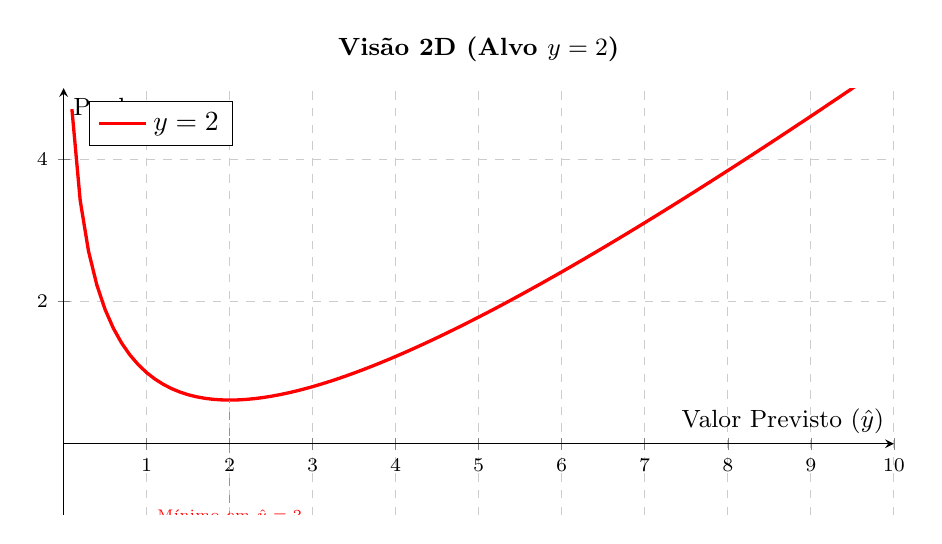
\begin{tikzpicture}
            \begin{axis}[
                width=\linewidth,  
                height=7cm,
                xlabel={Valor Previsto ($\hat{y}$)},
                ylabel={Perda},
                axis lines=middle,
                grid=major,
                grid style={dashed, gray!40},
                xmin=0, xmax=10,
                ymin=-1, ymax=5,
                legend pos=north west,
                title style={font=\bfseries\small},
                label style={font=\small},
                tick label style={font=\scriptsize},
                title={Visão 2D (Alvo $y=2$)}
            ]
                % Perda Poisson: x - y*ln(x) -> Aqui x é y_hat, y fixo em 2
                \addplot[domain=0.1:10, samples=100, color=red, very thick] {x - 2*ln(x)};
                \addlegendentry{$y=2$}
                
                % Linha pontilhada no mínimo
                \draw[dashed, red!60] (axis cs:2, -2) -- (axis cs:2, {2-2*ln(2)});
                \node[anchor=north, font=\tiny, text=red] at (axis cs:2, -0.8) {Mínimo em $\hat{y}=2$};
            \end{axis}
        \end{tikzpicture}
        \caption{Comportamento para valor real baixo.}%
        \label{fig:poisson-2d-low}
    \end{subfigure}
    \hfill
    \begin{subfigure}[b]{0.48\textwidth}
        \centering
        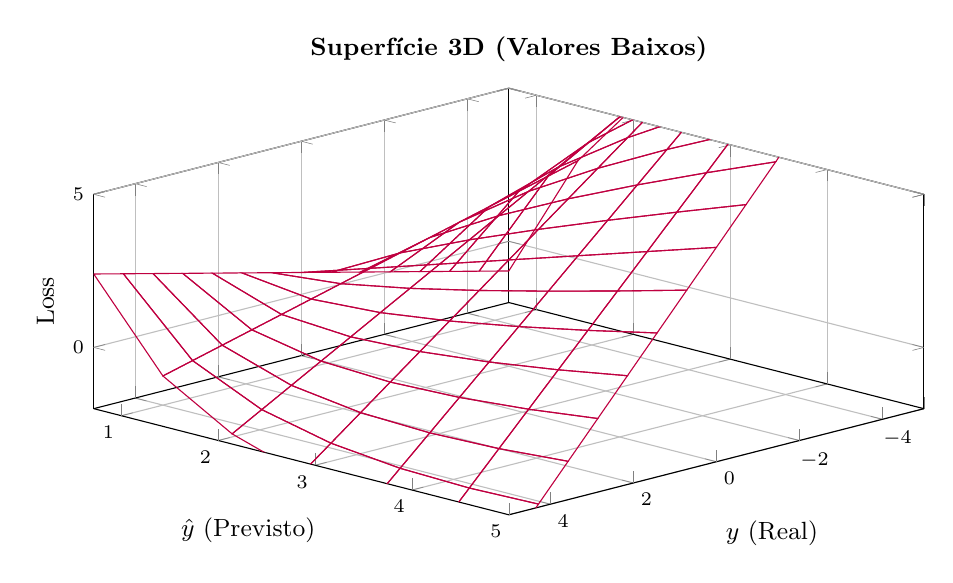
\begin{tikzpicture}
            \begin{axis}[
                width=\linewidth,
                height=7cm,
                xlabel={$y$ (Real)},
                ylabel={$\hat{y}$ (Previsto)},
                zlabel={Loss},
                grid=major,
                view={135}{35}, % Angulo de visão
                legend pos=north east,
                title style={font=\bfseries\small},
                label style={font=\small},
                tick label style={font=\scriptsize},
                title={Superfície 3D (Valores Baixos)},
                zmin=-2, zmax=5
            ]
                \addplot3[
                    mesh,           
                    color=purple,   % Cor consistente com o gráfico 2D
                    shader=interp,  
                    domain=-5:5,    % Mesmo domínio do seu template
                    domain y=-5:5,  % Mesmo domínio do seu template
                    samples=15      % Mesma resolução da malha
                ] { y - x*ln(y) };
            \end{axis}
        \end{tikzpicture}
        \caption{Superfície local (Região $1 \le y \le 5$).}%
        \label{fig:poisson-3d-low}
    \end{subfigure}

    \vspace{0.5cm} 

    \begin{subfigure}[b]{0.48\textwidth}
        \centering
        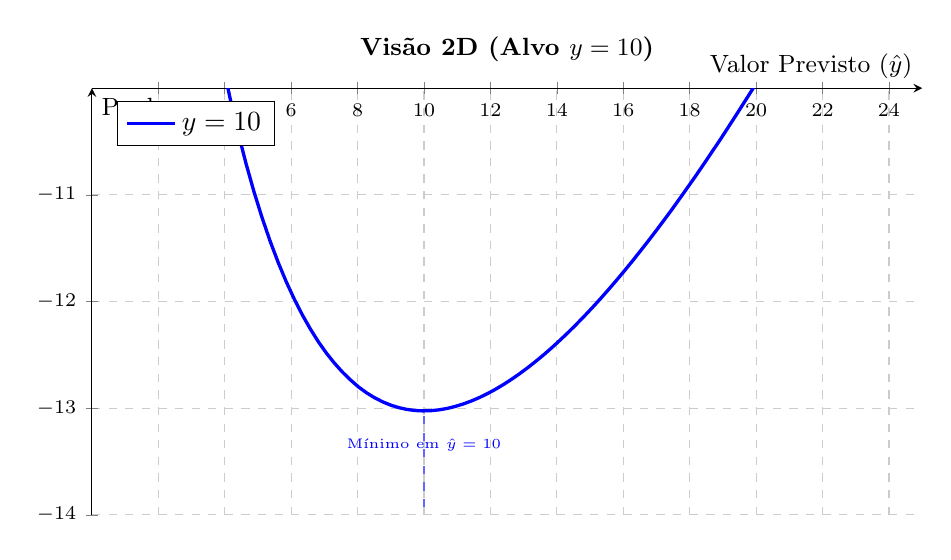
\begin{tikzpicture}
            \begin{axis}[
                width=\linewidth,  
                height=7cm,
                xlabel={Valor Previsto ($\hat{y}$)},
                ylabel={Perda},
                axis lines=middle,
                grid=major,
                grid style={dashed, gray!40},
                xmin=0, xmax=25,
                % Ajustando ymin/ymax para focar na curvatura
                ymin=-14, ymax=-10, 
                legend pos=north west,
                title style={font=\bfseries\small},
                label style={font=\small},
                tick label style={font=\scriptsize},
                title={Visão 2D (Alvo $y=10$)}
            ]
                % Perda Poisson para y=10
                \addplot[domain=1:25, samples=100, color=blue, very thick] {x - 10*ln(x)};
                \addlegendentry{$y=10$}
                
                % Linha pontilhada no mínimo
                \draw[dashed, blue!60] (axis cs:10, -20) -- (axis cs:10, {10-10*ln(10)});
                 \node[anchor=north, font=\tiny, text=blue] at (axis cs:10, -13.2) {Mínimo em $\hat{y}=10$};
            \end{axis}
        \end{tikzpicture}
        \caption{Comportamento para valor real alto.}%
        \label{fig:poisson-2d-high}
    \end{subfigure}
    \hfill
    \begin{subfigure}[b]{0.48\textwidth}
        \centering
        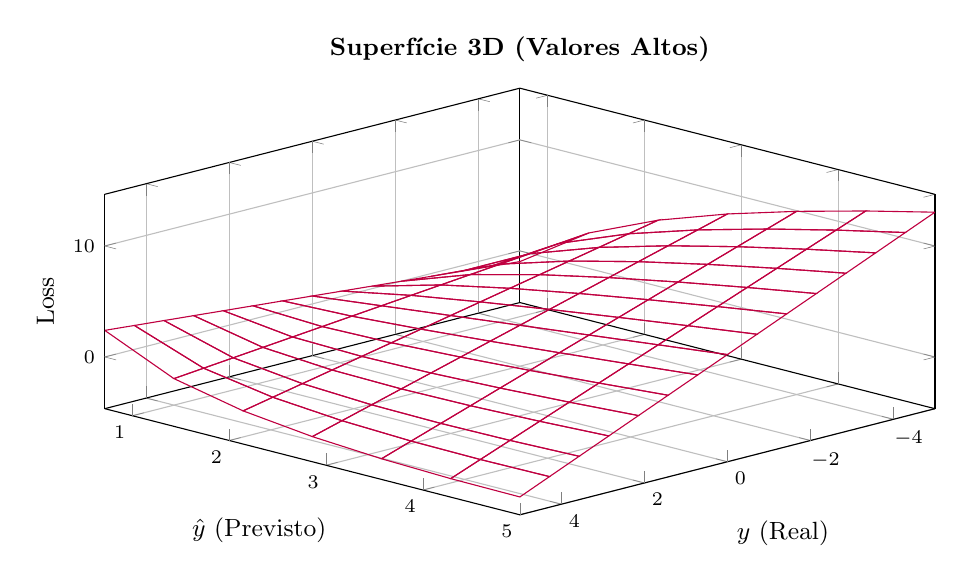
\begin{tikzpicture}
            \begin{axis}[
                width=\linewidth,
                height=7cm,
                xlabel={$y$ (Real)},
                ylabel={$\hat{y}$ (Previsto)},
                zlabel={Loss},
                grid=major,
                view={135}{35},
                title style={font=\bfseries\small},
                label style={font=\small},
                tick label style={font=\scriptsize},
                title={Superfície 3D (Valores Altos)}
            ]
                % Formula: y - x * ln(y) (x=Real, y=Previsto)
                \addplot3[
                    mesh,           
                    color=purple,   % Cor consistente com o gráfico 2D
                    shader=interp,  
                    domain=-5:5,    % Mesmo domínio do seu template
                    domain y=-5:5,  % Mesmo domínio do seu template
                    samples=15      % Mesma resolução da malha
                ] { y - x*ln(y) };
            \end{axis}
        \end{tikzpicture}
        \caption{Superfície local (Região $8 \le y \le 12$).}%
        \label{fig:poisson-3d-high}
    \end{subfigure}

    \caption{Comparação da Perda de Poisson ($L = \hat{y} - y \ln \hat{y}$) para diferentes magnitudes de $y$. Observe como a convexidade é mais ``apertada'' para valores pequenos e se alarga para valores grandes.}%
    \label{fig:poisson-loss-grid}
    \fonte{O autor (2025).}
\end{figure}

\medskip
\begin{center}
 * * *
\end{center}
\medskip

\textbf{Características da Perda de Poisson}
\vspace{1em}

\begin{itemize}
    \item \textbf{Convexa:} Umas das vantagens de se utilizar a perda de Poisson, está no fato dela ser uma função convexa, o que facilita para que os otimizadores baseados em gradiente consigam mais facilmente encontrar um ponto de mínimo global, ou chegar muito próximo dele, casos estejam configurados com os parâmetros ideais.
    \item \textbf{Continuidade e Suavidade:} Além de ser uma função convexa, a perda de Poisson também é uma função contínua e suave, isso se dá devido ao fato de não fazer o uso de cálculos que possam causar ``bicos'' nos seus gráficos, como o uso de módulos para calcular o valor absoluto. Se a função é suave e contínua, ela também se torna chamativa para ser utilizada em conjunto com otimizadores baseados em gradiente, pois estes não encontrarão dificuldades para percorrer a superfície da função.
    \item \textbf{Não-negatividade e Link Functions:} \textcite{LossesArticle} explicam que como dados de contagem não podem ser negativos, deve-se atentar com os valores preditos pelo modelo $\hat{y}_j$, pois eles deverão estar restritos em $\hat{y}_j > 0$. Os autores explicam que em modelos lineares generalizados a função exponencial é comumente utilizada como uma link function para garantir que esses valores se encaixem nesse intervalo \parencite{LossesArticle}. Dessa forma é possível discutir uma versão alternativa para descrever a perda de Poisson considerando que $\text{exp}$ está sendo usada como uma link function.
    
    Sabemos que um modelo de aprendizado de máquina, geralmente retorna algo que segue o padrão mostrado na Equação xxx
 
    \begin{equation}
        \hat{y}_j = \textbf{W}^T x_j + b
    \end{equation}

    Esse valor pode ser negativo e queremos que ele fique em um intervalo $\hat{y} > 0$. Então como \textcite{LossesArticle} sugerem, uma das soluções é utilizar a função exponencial como uma link function, então escrevemos

    \[
        \hat{y}_j = \text{exp}(\textbf{W}^T x_j + b)
    \]

    Ao substituir essa expressão na Equação~\ref{eq:poisson-loss}, que mostra a função de perda de Poisson, é possível chegar Em

    \[
        \Loss_{\text{Poisson}}(y_j, \hat{y}_j) = \sum_{j = 0}^N \text{exp}(\textbf{W}^T x_j + b) - y_j \log(\text{exp}(\textbf{W}^T x_j + b))
    \]

    É possível simplificar os cálculos do logaritmo, resultando na expressão

    \[
        \Loss_{\text{Poisson}}(y_j, \hat{y}_j) = \sum_{j = 0}^N \text{exp}(\textbf{W}^T x_j + b) - y_j  (\text{exp}(\textbf{W}^T x_j + b))
    \]

    A qual pode ser reescrita uma última vez como 

    \[
        \Loss_{\text{Poisson}}(y_j, \hat{y}_j) = \sum_{j = 0}^N \text{exp}(\hat{y}_j) - y_j  (\text{exp}(\hat{y}_j))
    \]

\end{itemize}

\medskip
\begin{center}
 * * *
\end{center}
\medskip

Vistas algumas propriedades dessa função, cabe também discutir a sua derivada, que será útil para a retropropagação do gradiente e o aprendizado do modelo. Calculando a derivada da perda de Poisson em relação aos valores preditos pelo modelo, é possível chegar na Equação~\ref{eq:poisson-loss-derivada}.

\begin{equacaodestaque}{Derivada da Perda de Poisson}
    \frac{\partial\Loss_{\text{Poisson}}}{\partial\hat{y}_j} = 1 -\frac{y_j}{\hat{y}_j} = \frac{\hat{y}_j -y_j}{\hat{y}_j}%
    \label{eq:poisson-loss-derivada}
\end{equacaodestaque}

Com base nessa equação, o próximo passo é plotar o gráfico dessa derivada, o qual pode ser visto na Figura~\ref{fig:poisson-loss-derivada}. Perceba que o gráfico foge do padrão visto até agora, é apenas a vista em duas dimensões da derivada, além disso, ele também apresenta curvas diferentes, para demonstrar como a função varia conforme os valores reais $y_j$ variam. Note que com a variação dos valores reais a curva da derivada começa a deslocar pelo plano do gráfico, para valores menores, como $y = 10$, são mais presentes no quarto quadrante, já em valores mais altos, $y = 2$ por exemplo, vão se aproximando mais do eixo das ordenadas.

\begin{figure}[h!]
    \centering
    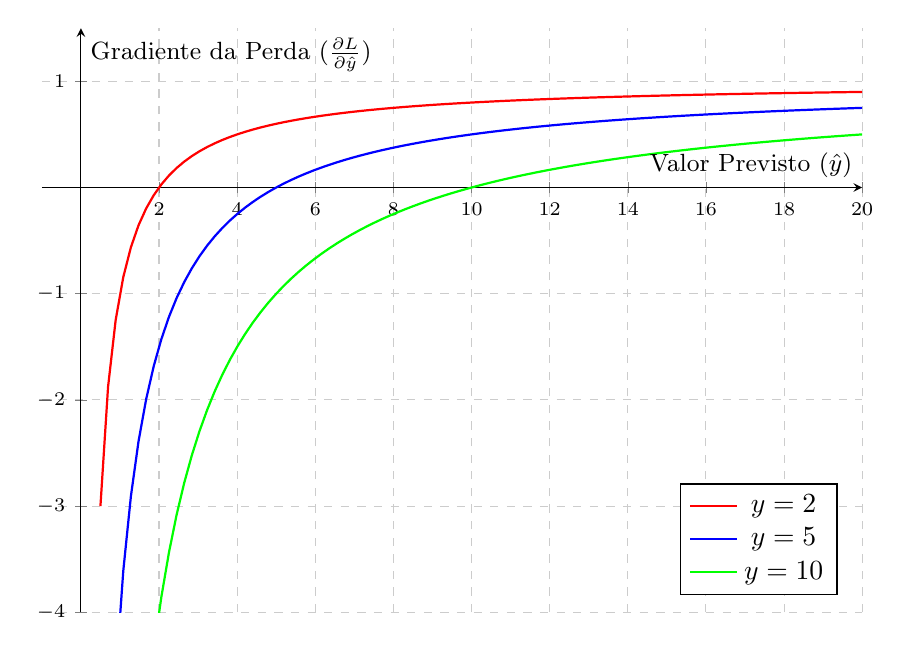
\begin{tikzpicture}
        \begin{axis}[
            xlabel={Valor Previsto ($\hat{y}$)},
            ylabel={Gradiente da Perda ($\frac{\partial L}{\partial \hat{y}}$)},
            axis lines=middle,
            grid=major,
            grid style={dashed, gray!40},
            xmin=-1, xmax=20,
            ymin=-4, ymax=1.5,
            legend pos=south east,
            width=12cm,
            height=9cm,
            title style={font=\bfseries},
            label style={font=\small},
            tick label style={font=\scriptsize}
        ]
            % Curva para y=2
            \addplot[domain=0.5:20, samples=101, color=red, thick] {1 - 2/x};
            \addlegendentry{$y=2$}
            
            % Curva para y=5
            \addplot[domain=0.5:20, samples=101, color=blue, thick] {1 - 5/x};
            \addlegendentry{$y=5$}

            % Curva para y=10
            \addplot[domain=0.5:20, samples=101, color=green, thick] {1 - 10/x};
            \addlegendentry{$y=10$}
            
        \end{axis}
    \end{tikzpicture}
    \caption{Gráfico da derivada da Perda de Poisson. O gradiente é zero quando $\hat{y}=y$ e assintótico a 1 para $\hat{y} \to \infty$.}%
    \label{fig:poisson-loss-derivada}
    \fonte{O autor (2025).}
\end{figure}

Além disso, como foi visto anteriormente, a função exponencial é utilizada como uma link function para resolver o problema dos dados da saída do modelo $\hat{y}$ serem sempre positivos, de forma que é possível escrever uma nova expressão, e até mais simplificada para o cenário em que $\text{exp}$ é combinada com a perda de Poisson para servir como uma link function. Dessa forma, essa expressão pode ser vista na Equação xx.

\begin{equacaodestaque}{Derivada da Perda de Poisson Com exp como Link Function}
    \frac{\partial\Loss_{\text{Poisson}}}{\partial\hat{y}_j} = \hat{y}_j - y_j%
    \label{eq:poisson-loss-com-link-function-derivada}
\end{equacaodestaque}

Dessa forma, a derivada passa ser a diferença entre o valor predito pelo modelo $\hat{y}_j$ com o valor real $y$.

\medskip
\begin{center}
 * * *
\end{center}
\medskip

\textbf{Algumas Aplicações da Perda de Poisson em Problemas de Regressão}%
\index{Aplicações práticas! Perda de Poisson}
\vspace{1em}

Por último, é importante discutir algumas das aplicações em que a perda de Poisson é utilizada. Para isso, é nítido ressaltar que ela estará relacionada com a distribuição de Poisson e com dados que segue essa distribuição, ou seja, que possuem a média igual a mediana. Usar a perda de Poisson para um cenário em que os dados seguem uma distribuição normal ou outro tipo de distribuição, não é algo ideal, uma vez que já existem funções que trabalham com essas situações. Um exemplo disso é o erro quadrático absoluto e sua relação com a distribuição Gaussiana.

Dito isso, vale citar os trabalhos:

\begin{itemize}
    \item \textbf{Aplicação 1 (Área):} Em \textit{Poisson regression in epidemiology}, \textcite{poisson-regression-in-epidemiology} faz uso da regressão de poisson para estimar os efeitos dos fatores de risco em incidência ou em taxas de mortalidade. Além disso, a regressão de Poisson também é utilizada no artigo para avaliar a relação dose-resposta para variáveis que representam níveis quantitativos de exposição \parencite{poisson-regression-in-epidemiology};
    \item \textbf{Predição de taxas de crime (Área):} Já em \textit{Poisson-Based Regression Analysis of Aggregate Crime Rates} \textcite{poisson-regression-for-crime-rates} utiliza modelos baseados na regressão de Poisson para analisar taxas de crime agregadas. O autor explica que no cenário em que estava trabalhando, a técnica de regressão por mínimos quadrados (a qual faz uso do erro quadrático médio, visto no início do capítulo), não é ideal, uma vez o tamanho da população de uma unidade agregada é pequeno quando comparado relativamente com a taxa de ofensas; de forma que as taxas de crime devem ser computadas a partir de um pequeno número de ofensas \parencite{poisson-regression-for-crime-rates};
    \item \textbf{Predição de sinistros em planos de saúde privados (Área):} Por fim, no trabalho \textit{Poisson regression and Zero-inflated Poisson regression: application to private health insurance data} \textcite{poisson-regression-and-zero-inflated-poisson-regression} utilizam a regressão de Poisson e uma técnica de regressão conhecida como regressão de Poisson zero-inflada, que é útil para dados que possuem um excesso de zeros. Para comparar e entender melhor qual técnica de regressão é mais interessante, os autores trabalham com o número de sinistros em um plano de saúde privado, no caso dos pesquisadores, o número de sinistros apresenta sobredispersão devido a predominância de zeros no conjunto de dados, de forma que a regressão de Poisson zero-inflada provou ser mais eficiente para lidar com esse tipo de problema \parencite{poisson-regression-and-zero-inflated-poisson-regression}.
\end{itemize}

\subsection{Deviância Gamma (Gamma Devience)}%
\index{Funções de Perda!Deviância Gamma (\textit{Gamma Devience})}

\textbf{A Distribuição Gamma}%
\index{Distribuição Gamma}
\vspace{1em}

\begin{equacaodestaque}{Distribuição Gamma (PDF)}
    f(y_j; k, \theta) = \frac{y_j^{k-1} e^{-y_j/\theta}}{\theta^k\Gamma(k)}%
    \label{eq:gamma-distribution-pdf}
\end{equacaodestaque}

\begin{figure}[h!]
    \centering % Centraliza a figura inteira
    
    % --- GRÁFICO 1: Forma Baixa (k=1) ---
    \begin{subfigure}[b]{0.48\textwidth}
        \centering
        \begin{tikzpicture}
            \begin{axis}[
                title={Distribuição Gamma ($k=1, \theta=2$)},
                xlabel={$x$ (valor contínuo)},
                ylabel={$f(x; k, \theta)$},
                smooth, % Linha contínua suave
                ymin=0,
                xmin=0, xmax=15,
                grid=major,
                grid style={dashed, gray!40},
                label style={font=\small},
                tick label style={font=\scriptsize}
            ]
            % Com k=1, theta=2: (x^0 * exp(-x/2)) / (2^1 * gamma(1)) = 0.5 * exp(-x/2)
            
            % <--- MUDANÇA AQUI ---
            % Substituindo a fórmula complexa pela sua função definida:
            \addplot[domain=0.01:15, samples=101, color=blue, thick] 
                { gamma_pdf(x, 1, 2) };
            \end{axis}
        \end{tikzpicture}
        \caption{Com forma $k=1$, a distribuição é uma exponencial decrescente.}%
        \label{fig:gamma-low-k}
    \end{subfigure}
    \hfill
    \begin{subfigure}[b]{0.48\textwidth}
        \centering
        \begin{tikzpicture}
            \begin{axis}[
                title={Distribuição Gamma ($k=3, \theta=2$)},
                xlabel={$x$ (valor contínuo)},
                ylabel={$f(x; k, \theta)$},
                smooth,
                ymin=0,
                xmin=0, xmax=20, % Range maior para ver a cauda
                grid=major,
                grid style={dashed, gray!40},
                label style={font=\small},
                tick label style={font=\scriptsize}
            ]
            % Com k=3, theta=2: (x^2 * exp(-x/2)) / (2^3 * gamma(3)) = (x^2 * exp(-x/2)) / 16
            
            % <--- MUDANÇA AQUI ---
            % Substituindo a fórmula complexa pela sua função definida:
            \addplot[domain=0.01:20, samples=101, color=red, thick] 
                { gamma_pdf(x, 3, 2) };
        
            % Média da Gamma = k * theta = 3 * 2 = 6
            % A altura do pico (0.166) foi calculada
            \draw[dashed, red!70] (axis cs:6, 0) -- (axis cs:6, 0.166); 
            \node[above, font=\tiny] at (axis cs:6, 0.166) {Média ($\mu=6$)};

            \end{axis}
        \end{tikzpicture}
        \caption{Com forma $k=3$, a distribuição tem um pico claro e uma cauda longa à direita (assimétrica).}%
        \label{fig:gamma-high-k}
    \end{subfigure}
    
    \caption{Comparação visual da Distribuição Gamma variando o parâmetro de forma $k$.}%
    \label{fig:gamma-comparison}
    \fonte{O autor (2025).}
\end{figure}

\medskip
\begin{center}
 * * *
\end{center}
\medskip

\begin{equacaodestaque}{Perda Gamma (\textit{Gamma Loss})}
    \Loss_{\text{Gamma}}(y_j, \hat{y}_j) = \log\left(\frac{\hat{y}_j}{y_j}\right) + \frac{y_j}{\hat{y}_j} -1%
    \label{eq:gamma-loss}
\end{equacaodestaque}

Em que:

\begin{itemize}
    \item $y_j$ representa o valor real da j-ésima amostra;
    \item $\hat{y}_j$ representa o valor predito pelo modelo;
    \item $N$ representa o número de amostras.
\end{itemize}

\begin{figure}[h!]
    \centering
    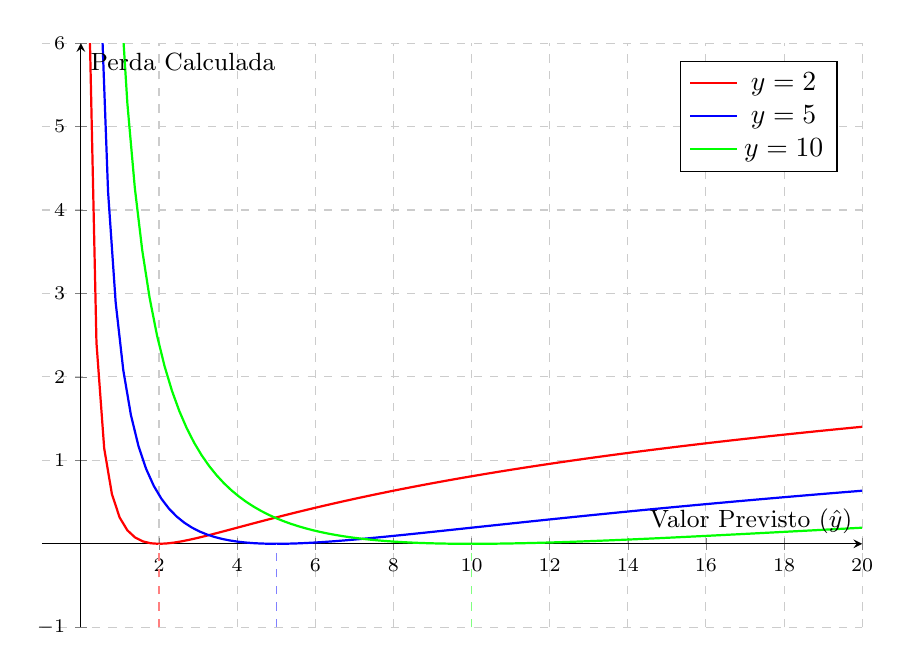
\begin{tikzpicture}
        \begin{axis}[
            xlabel={Valor Previsto ($\hat{y}$)},
            ylabel={Perda Calculada},
            axis lines=middle,
            grid=major,
            grid style={dashed, gray!40},
            xmin=-1, xmax=20,
            ymin=-1, ymax=6,  % Ajustado para melhor visualização da Gamma
            legend pos=north east, % Movido para um local melhor
            width=12cm,
            height=9cm,
            title style={font=\bfseries},
            label style={font=\small},
            tick label style={font=\scriptsize}
        ]
            % Fórmula: ln(x/y) + (y/x) - 1
            
            % Curva para y=2
            \addplot[domain=0.2:20, samples=101, color=red, thick] {ln(x/2) + (2/x) - 1};
            \addlegendentry{$y=2$}
            % Mínimo em y=2, perda=0
            \draw[dashed, red!50] (axis cs:2, -1) -- (axis cs:2, 0);

            % Curva para y=5
            \addplot[domain=0.5:20, samples=101, color=blue, thick] {ln(x/5) + (5/x) - 1};
            \addlegendentry{$y=5$}
            % Mínimo em y=5, perda=0
            \draw[dashed, blue!50] (axis cs:5, -1) -- (axis cs:5, 0);

            % Curva para y=10
            \addplot[domain=1:20, samples=101, color=green, thick] {ln(x/10) + (10/x) - 1};
            \addlegendentry{$y=10$}
            % Mínimo em y=10, perda=0
            \draw[dashed, green!50] (axis cs:10, -1) -- (axis cs:10, 0);
            
        \end{axis}
    \end{tikzpicture}
    \caption{Gráfico da Perda Gamma para diferentes valores reais de $y$. O mínimo de cada curva (Perda = 0) ocorre em $\hat{y}=y$.}%
    \label{fig:gamma-loss}
    \fonte{O autor (2025).}
\end{figure}

\medskip
\begin{center}
 * * *
\end{center}
\medskip

\textbf{Características da Deviância Gamma}
\vspace{1em}

\begin{itemize}
    \item \textbf{Característica 1:}
    \item \textbf{Característica 2:}
    \item \textbf{Característica 3:}
\end{itemize}

\medskip
\begin{center}
 * * *
\end{center}
\medskip

\begin{equacaodestaque}{Derivada da Perda Gamma}
    \frac{\partial\Loss_{\text{Gamma}}}{\partial\hat{y}_j} = \frac{1}{\hat{y}_j} -\frac{y_j}{\hat{y}_j^2} = \frac{\hat{y}_j -y_j}{\hat{y}_j^2}%
    \label{eq:gamma-loss-derivada}
\end{equacaodestaque}

\begin{figure}[h!]
    \centering
    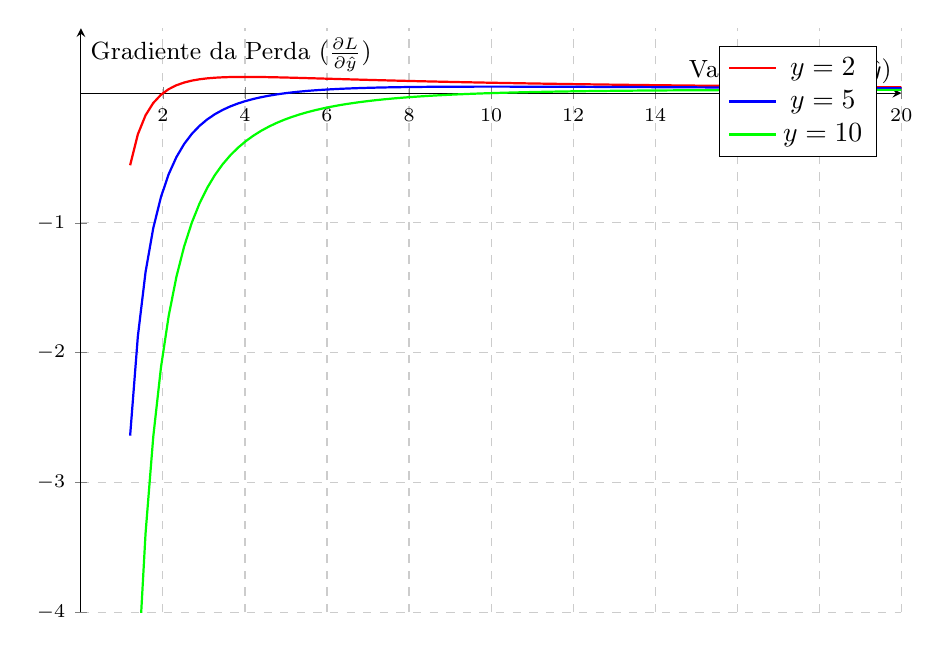
\begin{tikzpicture}
        \begin{axis}[
            xlabel={Valor Previsto ($\hat{y}$)},
            ylabel={Gradiente da Perda ($\frac{\partial L}{\partial \hat{y}}$)},
            axis lines=middle,
            grid=major,
            grid style={dashed, gray!40},
            xmin=0, xmax=20,  % Ajustado para a derivada da Gamma
            ymin=-4, ymax=0.5,   % Ajustado para a derivada da Gamma
            legend pos=north east, % Movido para um local melhor
            width=12cm,
            height=9cm,
            title style={font=\bfseries},
            label style={font=\small},
            tick label style={font=\scriptsize}
        ]
            % Fórmula: (x - y) / (x^2)
            
            % Curva para y=2
            \addplot[domain=1.2:20, samples=101, color=red, thick] {(x - 2) / (x^2)};
            \addlegendentry{$y=2$}
            
            % Curva para y=5
            \addplot[domain=1.2:20, samples=101, color=blue, thick] {(x - 5) / (x^2)};
            \addlegendentry{$y=5$}

            % Curva para y=10
            \addplot[domain=1.2:20, samples=101, color=green, thick] {(x - 10) / (x^2)};
            \addlegendentry{$y=10$}
            
        \end{axis}
    \end{tikzpicture}
    \caption{Gráfico da derivada da Perda Gamma. O gradiente é zero quando $\hat{y}=y$ e assintótico a 0 para $\hat{y} \to \infty$.}%
    \label{fig:gamma-loss-derivada}
    \fonte{O autor (2025).}
\end{figure}

\medskip
\begin{center}
 * * *
\end{center}
\medskip

\textbf{Algumas Aplicações da Deviância Gamma em Problemas de Regressão}%
\index{Aplicações práticas! Deviância Gamma}
\vspace{1em}

\begin{itemize}
    \item \textbf{Aplicação 1 (Área):}
    \item \textbf{Aplicação 2 (Área):}
    \item \textbf{Aplicação 3 (Área):}
    \item \textbf{Aplicação 4 (Área):}
\end{itemize}

\subsection{Perda de Tweedie (Tweedie Loss)}%
\index{Funções de Perda!Perda de Tweedie (\textit{Tweedie Loss})}

\begin{equacaodestaque}{Perda de Tweedie (\textit{Tweedie Loss})}
    \Loss_{\text{Tweedie}}(y_j, \hat{y}_j; p) = -\frac{y_j \cdot \hat{y}_j^{1-p}}{1-p} + \frac{\hat{y}_j^{2-p}}{2-p}%
    \label{eq:tweedie-loss}
\end{equacaodestaque}

Em que:

\begin{itemize}
    \item $y_j$ representa o valor real da j-ésima amostra;
    \item $\hat{y}_j$ representa o valor predito pelo modelo;
    \item $N$ representa o número de amostras.
\end{itemize}

\begin{figure}[h!]
    \centering
    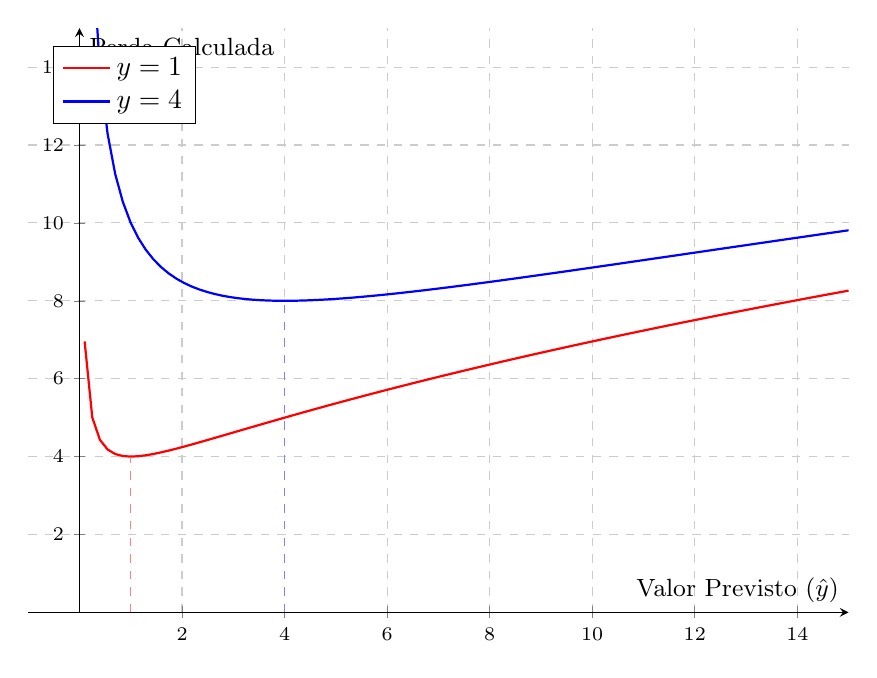
\begin{tikzpicture}
        \begin{axis}[
            xlabel={Valor Previsto ($\hat{y}$)},
            ylabel={Perda Calculada},
            axis lines=middle,
            grid=major,
            grid style={dashed, gray!40},
            xmin=-1, xmax=15,
            ymin=0, ymax=15,
            legend pos=north west,
            width=12cm,
            height=9cm,
            title style={font=\bfseries},
            label style={font=\small},
            tick label style={font=\scriptsize}
        ]
            % Definição do parâmetro p
            \def\p{1.5}

            % Curva para y=1
            \addplot[domain=0.1:15, samples=101, color=red, thick] 
                { -1*x^(1-\p)/(1-\p) + x^(2-\p)/(2-\p) };
            \addlegendentry{$y=1$}
            \draw[dashed, red!50] (axis cs:1, 0) -- (axis cs:1, {-1*1^(1-\p)/(1-\p) + 1^(2-\p)/(2-\p)});

            % Curva para y=4
            \addplot[domain=0.1:15, samples=101, color=blue, thick] 
                { -4*x^(1-\p)/(1-\p) + x^(2-\p)/(2-\p) };
            \addlegendentry{$y=4$}
            \draw[dashed, blue!50] (axis cs:4, 0) -- (axis cs:4, {-4*4^(1-\p)/(1-\p) + 4^(2-\p)/(2-\p)});
            
        \end{axis}
    \end{tikzpicture}
    \caption{Gráfico da Perda de Tweedie para $p=1.5$. O mínimo de cada curva ocorre em $\hat{y}=y$.}%
    \label{fig:tweedie-loss}
    \fonte{O autor (2025).}
\end{figure}

\medskip
\begin{center}
 * * *
\end{center}
\medskip

\textbf{Características da Perda de Tweedie}
\vspace{1em}

\begin{itemize}
    \item \textbf{Característica 1:}
    \item \textbf{Característica 2:}
    \item \textbf{Característica 3:}
\end{itemize}

\medskip
\begin{center}
 * * *
\end{center}
\medskip

\begin{equacaodestaque}{Derivada da Perda de Tweedie}
    \frac{\partial\Loss_{\text{Tweedie}}}{\partial\hat{y}_j} = \hat{y}_j^{-p}(\hat{y}_j -y_j)%
    \label{eq:tweedie-loss-derivada}
\end{equacaodestaque}

\begin{figure}[h!]
    \centering
    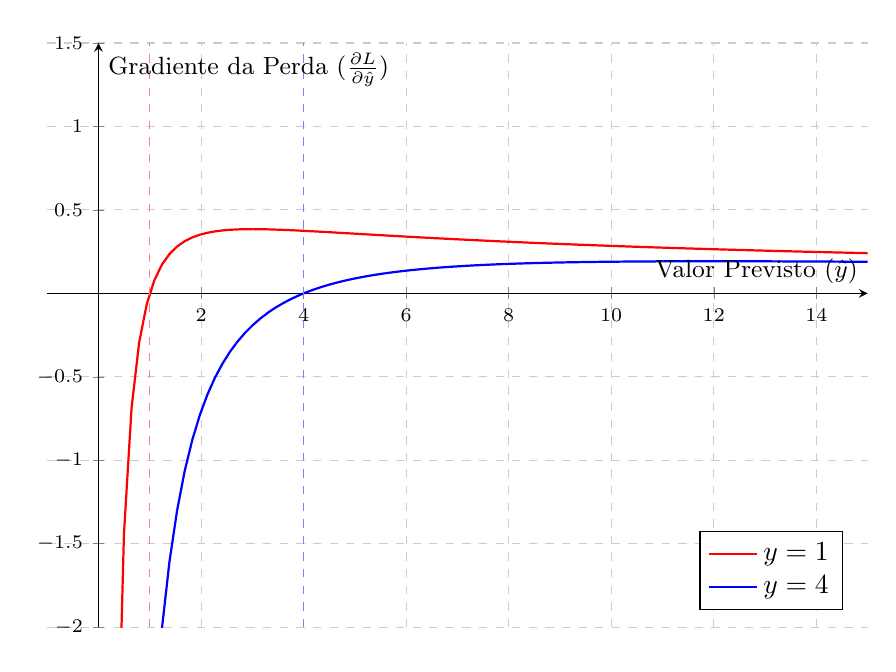
\begin{tikzpicture}
        \begin{axis}[
            xlabel={Valor Previsto ($\hat{y}$)},
            ylabel={Gradiente da Perda ($\frac{\partial L}{\partial \hat{y}}$)},
            axis lines=middle,
            grid=major,
            grid style={dashed, gray!40},
            xmin=-1, xmax=15,
            ymin=-2, ymax=1.5,
            legend pos=south east,
            width=12cm,
            height=9cm,
            title style={font=\bfseries},
            label style={font=\small},
            tick label style={font=\scriptsize}
        ]
            % Definição do parâmetro p
            \def\p{1.5}
            
            % Curva para y=1
            \addplot[domain=0.2:15, samples=101, color=red, thick] 
                {x^(-\p)*(x-1)};
            \addlegendentry{$y=1$}
            
            % Curva para y=4
            \addplot[domain=0.2:15, samples=101, color=blue, thick] 
                {x^(-\p)*(x-4)};
            \addlegendentry{$y=4$}

            % Linhas verticais onde o gradiente é zero
            \draw[dashed, red!50] (axis cs:1, -2) -- (axis cs:1, 1.5);
            \draw[dashed, blue!50] (axis cs:4, -2) -- (axis cs:4, 1.5);
            
        \end{axis}
    \end{tikzpicture}
    \caption{Gráfico da derivada da Perda de Tweedie para $p=1.5$. O gradiente é zero quando a previsão é igual ao valor real.}%
    \label{fig:tweedie-loss-derivada}
    \fonte{O autor (2025).}
\end{figure}

\medskip
\begin{center}
 * * *
\end{center}
\medskip

\textbf{Algumas Aplicações da Perda de Tweedie}%
\index{Aplicações práticas! Perda de Tweedie}
\vspace{1em}

\begin{itemize}
    \item \textbf{Aplicação 1 (Área):}
    \item \textbf{Aplicação 2 (Área):}
    \item \textbf{Aplicação 3 (Área):}
    \item \textbf{Aplicação 4 (Área):}
\end{itemize}

\subsection{Divergência Kullback-Leibler}%
\index{Funções de Perda!Divergência de Kullback-Leibler}

\begin{equacaodestaque}{Divergência KL entre duas Gaussianas}
    D_{KL}(P || Q) = \log\frac{\sigma_2}{\sigma_1} + \frac{\sigma_1^2 + (\mu_1 -\mu_2)^2}{2\sigma_2^2} -\frac{1}{2}%
    \label{eq:kl-divergence-gaussiana}
\end{equacaodestaque}

\begin{figure}[h!]
    \centering
    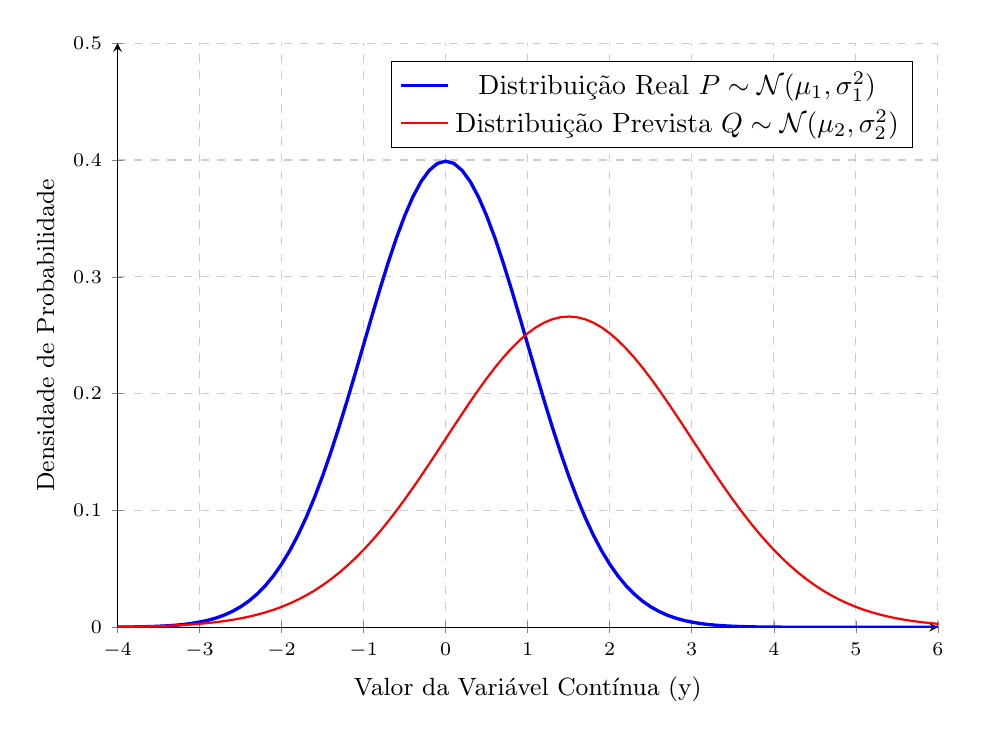
\begin{tikzpicture}
        \begin{axis}[
            xlabel={Valor da Variável Contínua (y)},
            ylabel={Densidade de Probabilidade},
            axis lines=left,
            grid=major,
            grid style={dashed, gray!40},
            xmin=-4, xmax=6,
            ymin=0, ymax=0.5,
            legend pos=north east,
            width=12cm,
            height=9cm,
            title style={font=\bfseries},
            label style={font=\small},
            tick label style={font=\scriptsize}
        ]
            % Distribuição Real P
            \addplot[
                domain=-4:6, samples=101, color=blue, very thick,
                ] {exp(-(x-0)^2 / (2*1^2)) / (1 * sqrt(2*pi))};
            \addlegendentry{Distribuição Real $P \sim \mathcal{N}(\mu_1, \sigma_1^2)$}

            % Distribuição Prevista Q
            \addplot[
                domain=-4:6, samples=101, color=red, thick,
            ] {exp(-(x-1.5)^2 / (2*1.5^2)) / (1.5 * sqrt(2*pi))};
            \addlegendentry{Distribuição Prevista $Q \sim \mathcal{N}(\mu_2, \sigma_2^2)$}
            
        \end{axis}
    \end{tikzpicture}
    \caption{A Divergência KL mede a diferença entre a distribuição prevista pelo modelo ($Q$) e a distribuição real dos dados ($P$).}%
    \label{fig:kl-divergence-concept-regressao}
    \fonte{O autor (2025).}
\end{figure}

\medskip
\begin{center}
 * * *
\end{center}
\medskip

\textbf{Características da Divergência de Kullback-Leibler} 
\vspace{1em}

\begin{itemize}
    \item \textbf{Característica 1:}
    \item \textbf{Característica 2:}
    \item \textbf{Característica 3:}
\end{itemize}

\medskip
\begin{center}
 * * *
\end{center}
\medskip

\begin{equacaodestaque}{Derivadas da Divergência KL (Gaussiana)}
    \frac{\partial D_{KL}}{\partial \mu_2} = \frac{\mu_2 -\mu_1}{\sigma_2^2}
    \\[10pt] % Espaçamento vertical
    \frac{\partial D_{KL}}{\partial \sigma_2} = \frac{1}{\sigma_2} -\frac{\sigma_1^2 + (\mu_1 -\mu_2)^2}{\sigma_2^3}%
    \label{eq:kl-divergence-derivada-gaussiana}
\end{equacaodestaque}

\medskip
\begin{center}
 * * *
\end{center}
\medskip

\textbf{Algumas Aplicações da Divergência de Kullback-Leibler em Problemas de Regressão}%
\index{Aplicações práticas! Divergência de Kullback-Leibler}
\vspace{1em}

\begin{itemize}
    \item \textbf{Aplicação 1 (Área):}
    \item \textbf{Aplicação 2 (Área):}
    \item \textbf{Aplicação 3 (Área):}
    \item \textbf{Aplicação 4 (Área):}
\end{itemize}

\section{Comparativo: Funções de Perda para Regressão}

\begin{table}[htbp]
    \centering
    \begin{threeparttable}
        \caption{Comparativo das funções das funções de perda para problemas de regressão}%
        \label{tab:comparativo-funcoes-de-perda-para-regressao}

        \begin{tabularx}{\textwidth}{p{3.2cm} *{1}{>{\raggedright\arraybackslash}X}}
            \toprule
            \textbf{Função} & \textbf{Principais características} \\
            \midrule
            Erro quadrático médio (\textit{MSE}) & -  \\
            \addlinespace
            Erro absoluto médio (\textit{MAE}) & - \\
            \addlinespace
            Perda de Huber (\textit{Huber loss}) & - \\
            \addlinespace
            Perda log-cosh (\textit{Log-cosh loss}) & - \\
            \addlinespace
            Erro quadrático logarítmico médio (\textit{MSLE}) & - \\
            \addlinespace
            Perda quantílica (\textit{Quantile loss}) & - \\
            \addlinespace
            Perda epsilon-insensível (\textit{$\epsilon$-insentive}) & - \\
            \addlinespace
            Perda de Poisson (\textit{Poisson loss}) & - \\
            \addlinespace
            Deviância Gamma (\textit{Poisson loss}) & - \\
            \addlinespace
            Perda de Tweedie (\textit{Tweedie loss}) & - \\
            \addlinespace
            Divergência de Kullback-Leibler (\textit{KL-divergence}) & - \\
            \addlinespace
        \end{tabularx}
        
        \begin{tablenotes}[para]
            \small
            \item[] Fonte: O autor (2025).
        \end{tablenotes}

    \end{threeparttable}
\end{table}

\section{Fluxograma: Escolhendo a Função de Perda Ideal}

\medskip
\begin{center}
 * * *
\end{center}
\medskip

\textbf{Indo Além das Funções de Perda Para Regressão}
\medskip

Nesse capítulo foi visto uma série de funções de perdas que tinham uma característica em comum: são utilizadas para lidar com problemas de regressão. Contudo, esse não é o único conjunto de funções de perda que existe. Existem funções de perda que são ideais para problemas de classificação, seja ele com duas classes (binário), ou multi-classe, essas funções são o tópico central do Capítulo~\ref{cap:perda-classificacao}. Além disso, existem vários outros tipos de problemas, alguns bem mais específicos, como reconhecer objetos em uma foto, para isso, o Capítulo~\ref{cap:perdas-especificas} busca fazer uma coletânea de outras funções de perda para situações mais específicas ao se construir um modelo de aprendizado de máquina.

Contudo, foram vistas apenas as funções de perda, e foi visto também que algumas podem servir como métricas, indicando de forma mais simples e direta se o modelo está performando bem ou não. Assim, um complemento para esse capítulo agora que você leitor conhece as funções de perda para regressão, é ler também o capítulo seguinte a este, o Capítulo~\ref{cap:metricas-de-avaliacao-para-regressao}. Ele é dedicado a explicar diferentes métricas que podem ser utilizadas para avaliar um modelo de regressão. De forma que será possível conhecer não só a função de perda ideal, mas também o conjunto de métricas ideais para avaliar o modelo desenvolvido.

\medskip
\begin{center}
 * * *
\end{center}
\medskip
